\newpage
\chapter{Simulation Results}
\label{ch:results}
In this chapter we study the impacts the parameters of the \MP method have on the simulation.
We start by varying the parameters of the explicit Harris and Crighton model one by one to study the effects.
Then we look at the collision damping term and why it is excluded from our investigation.
Afterward we conduct a parameter study where we vary two parameters at a time and compare the results to data kindly provided by the "Division of Combustion Technology" of the "Engler-Bunte-Institute" \footnote{\url{https://vbt.ebi.kit.edu/english/21_1186.php}}.
We look at the simulation with the parameters from the parameter study.
Lastly we look at one shortcoming of the \MP method.

\section{Single Parameter Testing}
In this section we study the effects of three parameters that are important in the explicit Harris and Crighton model
\begin{equation*}
    \ss = \dfrac{P_s \pvf^\beta}{\max [( \pvfcp - \pvf), \varepsilon ( 1- \pvf)]}
\end{equation*}
the close pack volume fraction $\pvfcp$, the exponent $\beta$ and the pressure constant $P_s$.
The single parameter testing and the collision damping testing was done earlier in this thesis. Therefor the grid is slightly modified to the grid described in the previous section.
Here we use a cuboid that has a side length of
$0.15 \operatorname{mm} \times \operatorname{mm} \times 100 \operatorname{mm}$ and a grid consisting of $1 \times 20 \times 100$ cells.
At time step zero $165251$ particles with a diameter of $0.05\operatorname{mm}$ are injected, spread out to a height of $25 \operatorname{mm}$.
Probes are taken at $1000$ points at $x = 0.075\operatorname{mm}$ (middle of the domain), and on a $20 \times 50$ grid on the domain $ [0\operatorname{mm},10\operatorname{mm}] \times [0\operatorname{mm},50\operatorname{mm}]$.


\subsection{Constant $\beta$}
In the reference Goldschmidt case, we have a quadratic dependency, therefore $\beta = 2$.
To explain the effect of $\beta$ on our simulation, we can rewrite the particle volume fraction as
\begin{align}
    \pvf = \alpha \pvfcp \qquad \lambda \in [0,1),
\end{align}
and insert it into a simplified version of the particle solid stress
\begin{align}
    \scs = \dfrac{P_s \pvf^\beta}{\pvfcp - \pvf} = \dfrac{\lambda^\beta}{(1-\lambda)} \pvfcp^{\beta -1}.
\end{align}
We can see from the first term that the solid particle stress diverges for the volume fraction approaching close pack. 
For smaller $\beta$, the leading factor rises faster, thus $\scs$ is higher for lower volume fractions. %In the plot for $\beta = 1$, we can observe this behavior in both the implicit \ref{fig:betaImp1} and the explicit \ref{fig:betaExp1} case, where the particles' position exceeds the plotted area.
With an increasing, $\beta$ the mean area in which particles are located shrinks.
Plotting the bed height for different values of $\beta$ reveals an exponential decay, see fig \ref{fig:meanBedBeta}
%\subsubsection{Explicit Case}
% \FloatBarrier
% \begin{figure}[h!]
% \captionsetup[subfigure]{
%   font={footnotesize},
%   %justification=raggedright,
%   singlelinecheck=false,
%   position=below,
%   %aboveskip=2.5cm, %belowskip=2.5cm,
%   skip=-0.7cm
%   %margin={0cm,-1cm}
% }
%     \centering
%     \begin{subfigure}[b]{0.49 \linewidth}
%     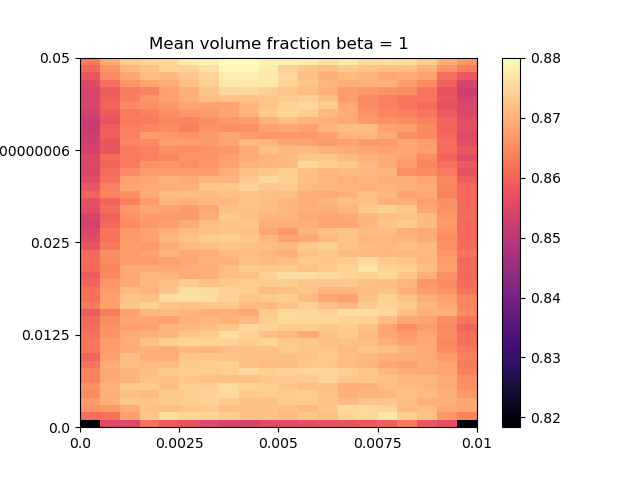
\includegraphics[width=0.9\linewidth]{sections/result/BetaExp/2d_apacked_1_0.00005_0.07.png}
%     \caption{}
%     \label{fig:betaExp1}
%     \end{subfigure}
%     \begin{subfigure}[b]{0.49 \linewidth}
%     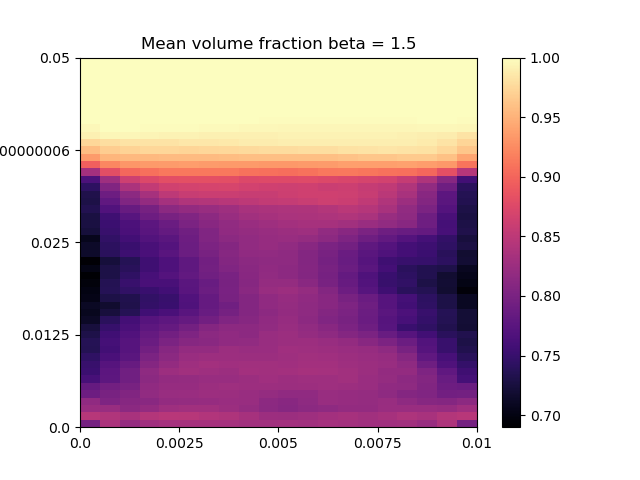
\includegraphics[width=0.9\linewidth]{sections/result/BetaExp/2d_apacked_1.5_0.00005_0.07.png}
%     \caption{}
%     \label{fig:betaExp2}
%     \end{subfigure}
%     \begin{subfigure}[b]{0.49 \linewidth}
%     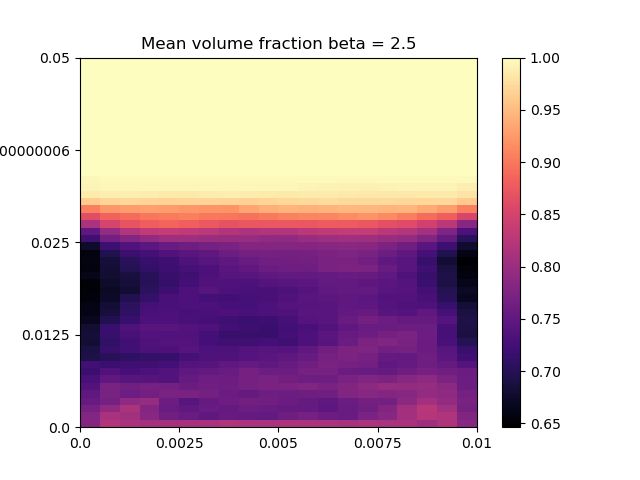
\includegraphics[width=0.9\linewidth]{sections/result/BetaExp/2d_apacked_2.5_0.00005_0.07.png}
%     \caption{}
%     \label{fig:betaExp3}
%     \end{subfigure}
%     \begin{subfigure}[b]{0.49 \linewidth}
%     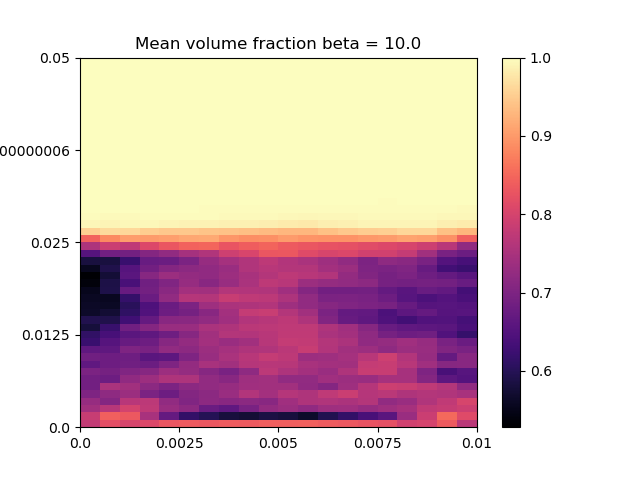
\includegraphics[width=0.9\linewidth]{sections/result/BetaExp/2d_apacked_10.0_0.00005_0.07.png}
%     \caption{}
%     \label{fig:betaExp4}
%     \end{subfigure}
%     %\caption{Mean particle volume fraction for $0.5s - 5s$ for different values of $\beta$. The packing model here is chosen as explicit.}
%     \label{fig:placeholder}
% %\end{figure}
% %\FloatBarrier
% %\subsubsection{Implicit Case}
% %\FloatBarrier
% %\begin{figure}
%     \begin{subfigure}[b]{0.49 \linewidth}
%     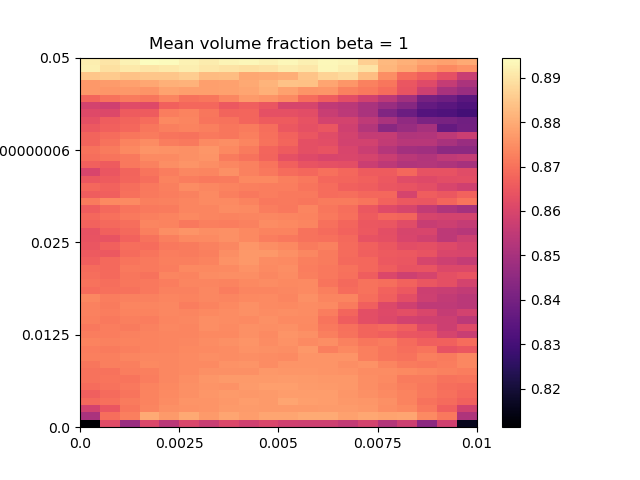
\includegraphics[width=0.9\linewidth]{sections/result/BetaImp/2d_apacked_1_0.00005_0.07.png}
%     \caption{}
%     \label{fig:betaImp1}
%     \end{subfigure}
%     \begin{subfigure}[b]{0.49 \linewidth}
%     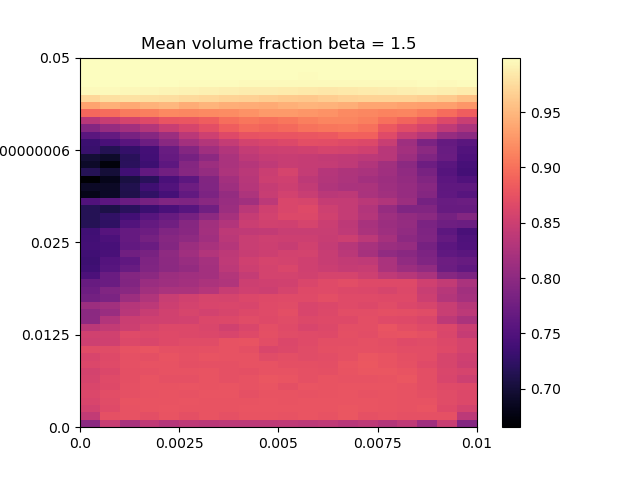
\includegraphics[width=0.9\linewidth]{sections/result/BetaImp/2d_apacked_1.5_0.00005_0.07.png}
%     \caption{}
%     \label{fig:betaImp2}
%     \end{subfigure}
%     \end{figure}
%     \begin{figure}[h!]\ContinuedFloat
%     \centering
%     \begin{subfigure}[b]{0.49 \linewidth}
%     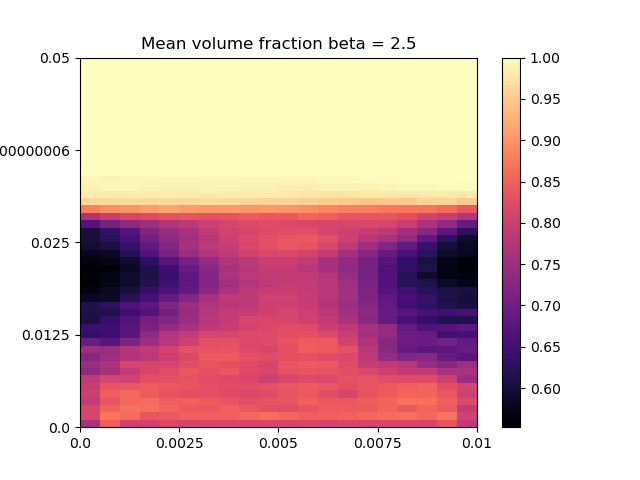
\includegraphics[width=0.9\linewidth]{sections/result/BetaImp/2d_apacked_2.5_0.00005_0.07.png}
%     \caption{}
%     \label{fig:betaImp3}
%     \end{subfigure}
%     \begin{subfigure}[b]{0.49 \linewidth}
%     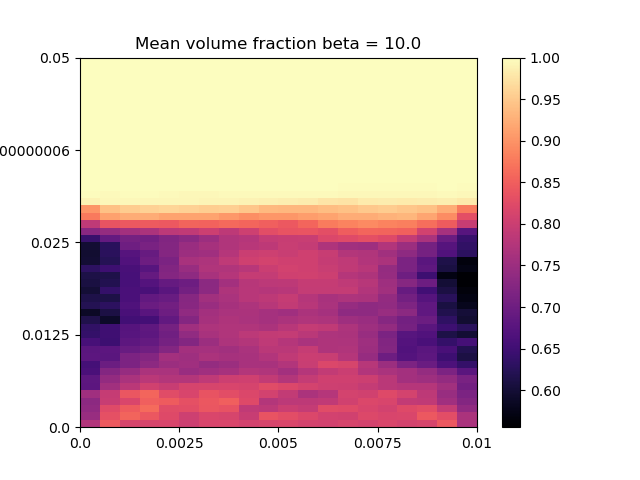
\includegraphics[width=0.9\linewidth]{sections/result/BetaImp/2d_apacked_10.0_0.00005_0.07.png}
%     \caption{}
%     \label{fig:betaImp4}
%     \end{subfigure}
%     \caption{Mean particle volume fraction at $0.5s - 5s$ for different values of $\beta$. With packing model explicit (\ref{fig:betaExp1}) - (\ref{fig:betaExp4}) and implicit (\ref{fig:betaImp1}) - (\ref{fig:betaImp4}).}
%     \label{fig:placeholder}
% \end{figure}
% \FloatBarrier
\begin{figure}[h!]
    \centering
    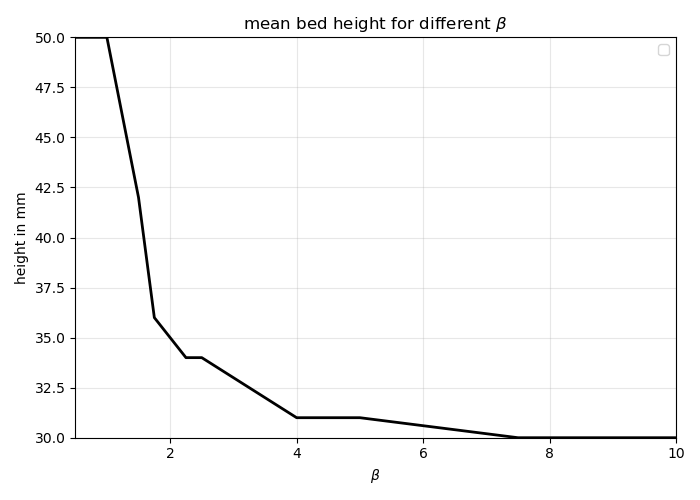
\includegraphics[width=0.55\linewidth]{sections/result/BetaExp/alphaExp.png}
    \caption{Mean bed height for different values of $\beta$. Bed heights exceeding $50mm$ are plotted as $50mm$.}
    \label{fig:meanBedBeta}
\end{figure}

\subsection{Solid pressure constant}
The solid pressure constant increases the solid particle stress linearly, which results in a linear increase in bed height, see figure \ref{fig:meanBedPS}.
A higher solid particle stress therefor leads to a higher bed. %, as observed in the following figure \ref{fig:pSolid}. The implicit case again leads to a higher bed height and a more pronounced hour-glass shape.
%\vspace{-1cm}

% \FloatBarrier
% \begin{figure}[h!]
% \captionsetup[subfigure]{
%   font={footnotesize},
%   %justification=raggedright,
%   singlelinecheck=false,
%   position=below,
%   %aboveskip=2.5cm, %belowskip=2.5cm,
%   skip=-0.9cm
%   %margin={0cm,-1cm}
% }
%     \centering
%     \vspace{-0.2cm}
%     \begin{subfigure}[t]{0.49 \linewidth}
%     %\caption{} 
%     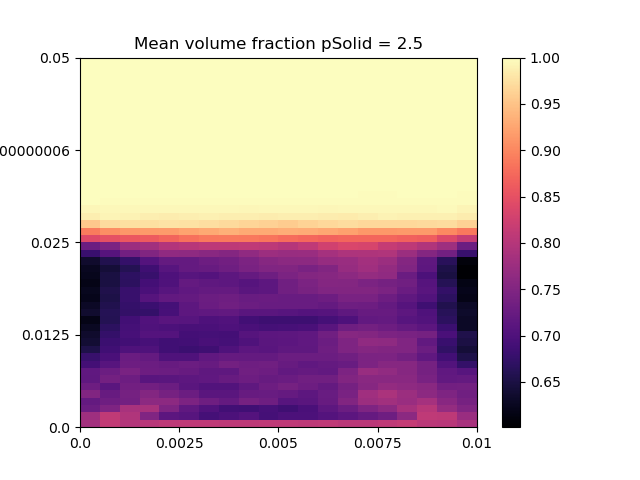
\includegraphics[width=0.9\linewidth]{sections/result/PSolidExp/2d_apacked_2.5_0.00005_0.07.png}
%     \caption{}
%     \label{fig:psolidExp1}
%     \end{subfigure}
%     \vspace{-0.2cm}
%     \begin{subfigure}[t]{0.49 \linewidth}
%     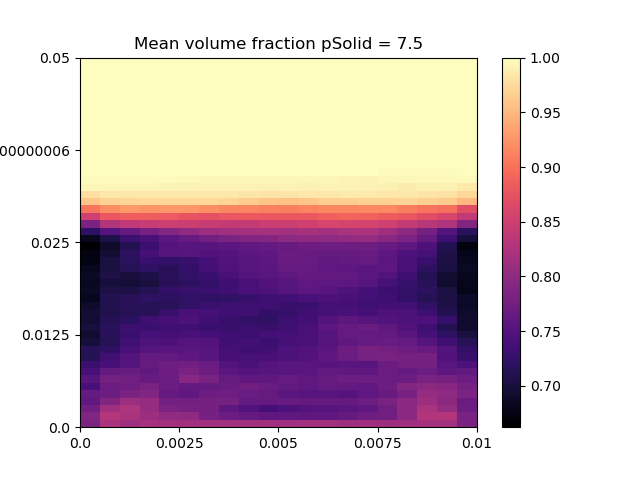
\includegraphics[width=0.9\linewidth]{sections/result/PSolidExp/2d_apacked_7.5_0.00005_0.07.png}
%     \caption{}
%     \label{fig:psolidExp2}
%     \end{subfigure}
%     \vspace{-0.15cm}
%     \begin{subfigure}[t]{0.49 \linewidth}
%     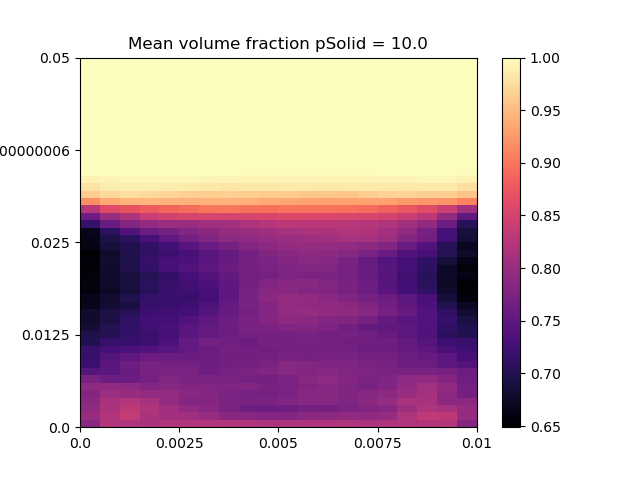
\includegraphics[width=0.9\linewidth]{sections/result/PSolidExp/2d_apacked_10.0_0.00005_0.07.png}
%     \caption{}
%     \label{fig:psolidExp3}
%     \end{subfigure}
%     \vspace{-0.15cm}
%     \begin{subfigure}[t]{0.49 \linewidth}
%     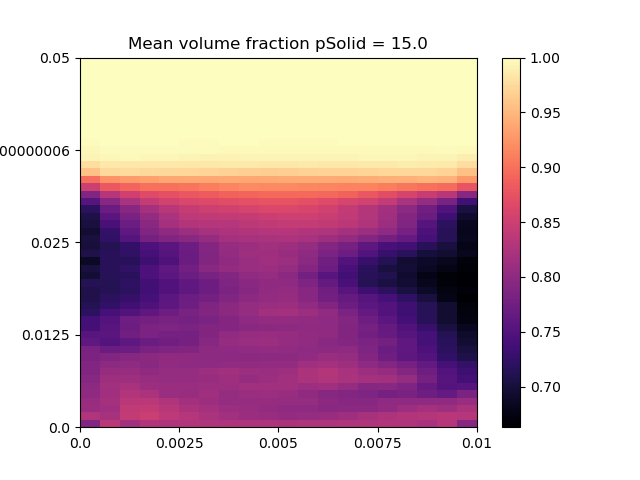
\includegraphics[width=0.9\linewidth]{sections/result/PSolidExp/2d_apacked_15.0_0.00005_0.07.png}
%     \caption{}
%     \label{fig:psolidExp4}
%     \end{subfigure}
%     \vspace{-0.15cm}
%     %\label{fig:placeholder}
% %\end{figure}
% %\FloatBarrier
% %\FloatBarrier
% %\begin{figure}
%     %\centering
%     \end{figure}
%     \begin{figure}[h!]\ContinuedFloat
%     \centering
%     \begin{subfigure}[t]{0.49 \linewidth}
%     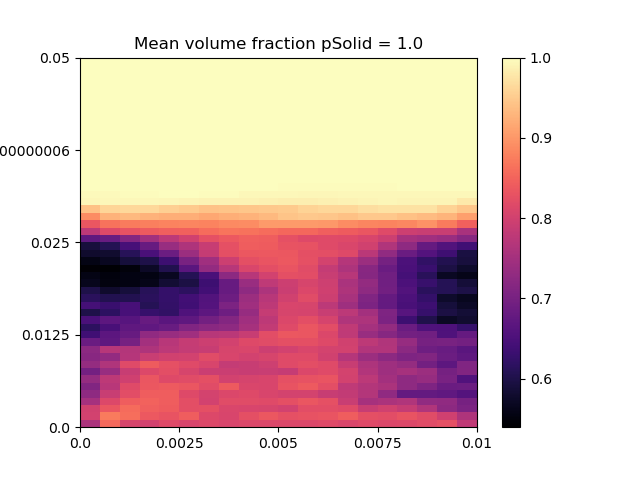
\includegraphics[width=0.9\linewidth]{sections/result/PSolidImp/2d_apacked_1.0_0.00005_0.07.png}
%     \caption{}
%     \label{fig:psolidImp1}
%     \end{subfigure}
%     \vspace{-0.15cm}
%     \begin{subfigure}[t]{0.49 \linewidth}
%     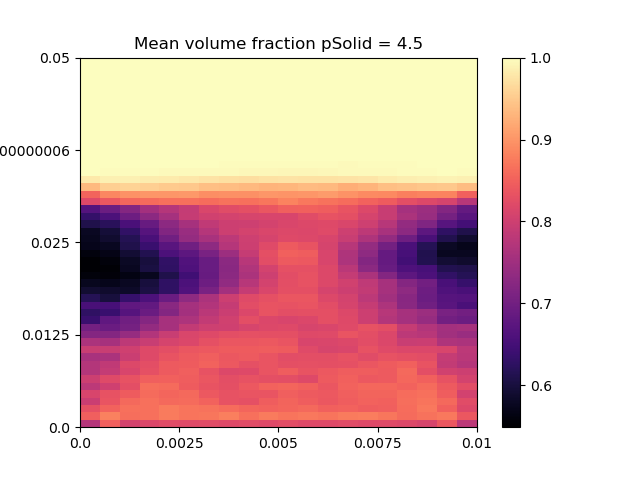
\includegraphics[width=0.9\linewidth]{sections/result/PSolidImp/2d_apacked_4.5_0.00005_0.07.png}
%     \caption{}
%     \label{fig:psolidImp2}
%     \end{subfigure}
%     \vspace{-0.15cm}
%     \end{figure}
%     \begin{figure}\ContinuedFloat
%     \begin{subfigure}[t]{0.49 \linewidth}
%     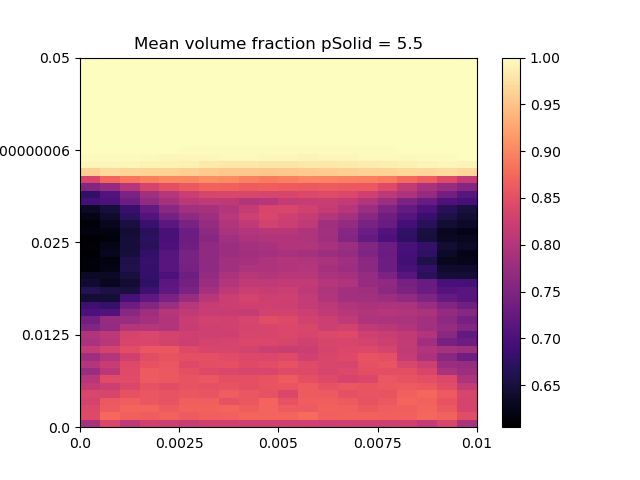
\includegraphics[width=0.9\linewidth]{sections/result/PSolidImp/2d_apacked_5.5_0.00005_0.07.png}
%     \caption{}
%     \label{fig:psolidImp3}
%     \end{subfigure}
%     \vspace{-0.15cm}
%     \begin{subfigure}[t]{0.49 \linewidth}
%     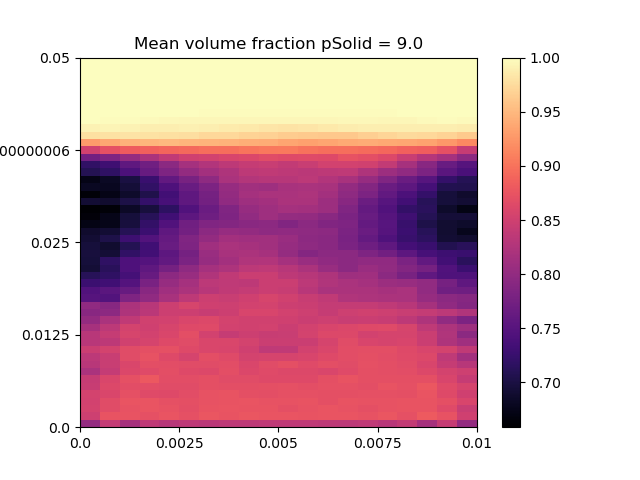
\includegraphics[width=0.9\linewidth]{sections/result/PSolidImp/2d_apacked_9.0_0.00005_0.07.png}
%     \caption{}
%     \label{fig:psolidImp4}
%     \end{subfigure}
%     \caption{Mean particle volume fraction for $0.5s - 5s$ for different values of $P_s$. With packing model explicit (\ref{fig:psolidExp1}) - (\ref{fig:psolidExp4}) and implicit (\ref{fig:psolidImp1}) - (\ref{fig:psolidImp4}).}
%     \label{fig:pSolid}
% \end{figure}
% \FloatBarrier
\begin{figure}[h!]
    \centering
    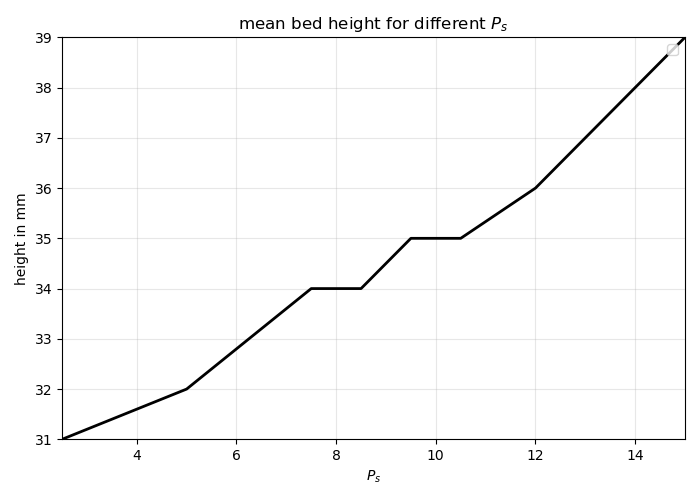
\includegraphics[width=0.55\linewidth]{sections/result/PSolidExp/alphaExp.png}
    \caption{Mean bed height for different values of $P_s
    $.}
    \label{fig:meanBedPS}
\end{figure}




\subsection{Volume fraction close packed}
Close to the close pack volume fraction, the solid particle stress increases rapidly. For a lower close pack volume fraction, the particles are accelerated for a lower volume fraction leading to a higher bed height, see figure \ref{fig:meanBedPacked}.
From experiments \cite{closePack}, we know that random sphere packing generally has a particle volume fraction of $0.63$, and the Kepler conjecture states that sphere packing cannot exceed $ \sim 0.74$. 
We can increase the close pack volume fraction of the particles further than what is theoretically possible, because the MP-PIC method does not check if the packing of spheres in a cell exceeds this limit, as particles are not modeled as spheres but as point masses. 
%For $\pvfcp = 0.85$ both the implicit and explicit case are stable, see figure \ref{fig:apackedExp4}, \ref{fig:apackedImp4}. In the implicit case, the simulation becomes unstable for a close pack volume fraction $\pvfcp = 0.95$.
%\vspace{-1cm}

\begin{figure}[h!]
    \centering
    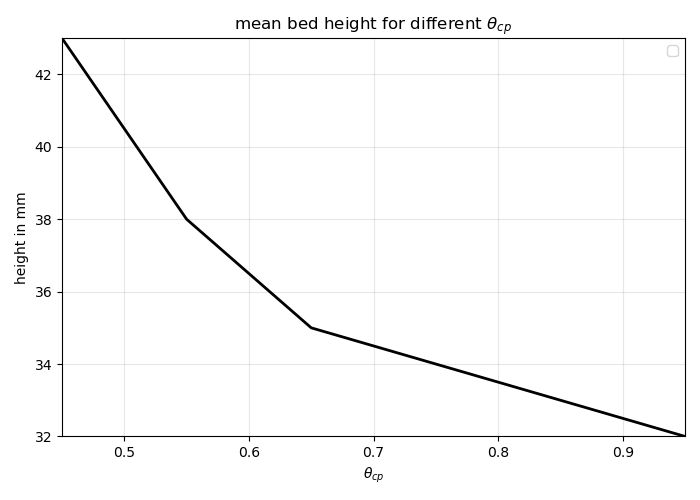
\includegraphics[width=0.55\linewidth]{sections/result/alphaPackedExp/alphaExp.png}
    \caption{Mean bed height for different values of $\pvfcp$.}
    \label{fig:meanBedPacked}
\end{figure}

% \FloatBarrier
% \begin{figure}[h!]
% \captionsetup[subfigure]{
%   font={footnotesize},
%   %justification=raggedright,
%   singlelinecheck=false,
%   position=below,
%   %aboveskip=2.5cm, %belowskip=2.5cm,
%   skip=-0.9cm
%   %margin={0cm,-1cm}
% }
%     \centering
%     \vspace{-0.2cm}
%     \begin{subfigure}[t]{0.49 \linewidth}
%     %\caption{} 
%     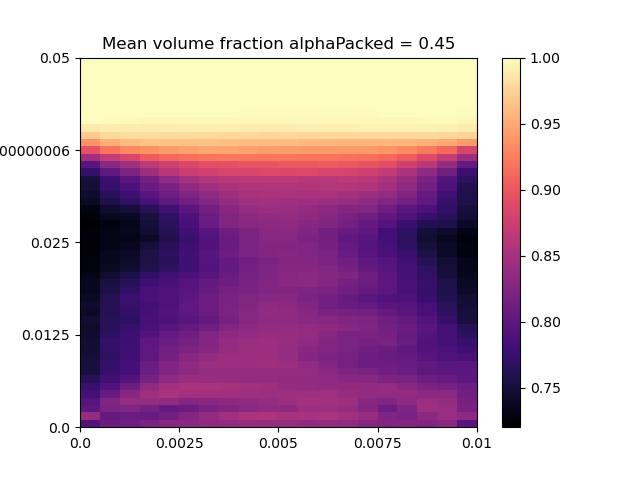
\includegraphics[width=0.9\linewidth]{sections/result/alphaPackedExp/2d_apacked_0.45_0.00005_0.07.png}
%     \caption{}
%     \label{fig:apackedExp1}
%     \end{subfigure}
%     \vspace{-0.2cm}
%     \begin{subfigure}[t]{0.49 \linewidth}
%     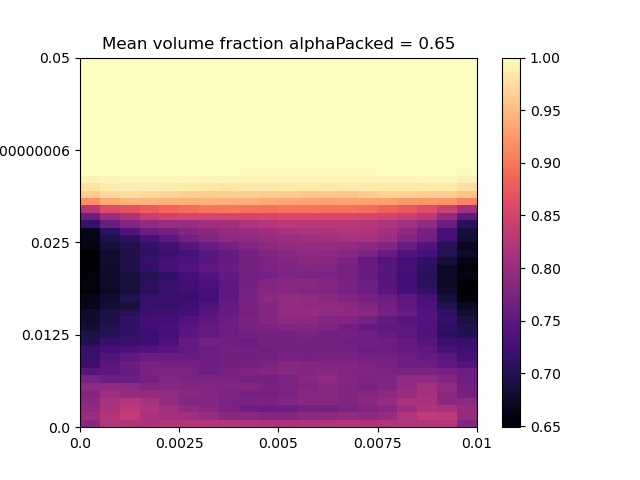
\includegraphics[width=0.9\linewidth]{sections/result/alphaPackedExp/2d_apacked_0.65_0.00005_0.07.png}
%     \caption{}
%     \label{fig:apackedExp2}
%     \end{subfigure}
%     \vspace{-0.15cm}
%     \begin{subfigure}[t]{0.49 \linewidth}
%     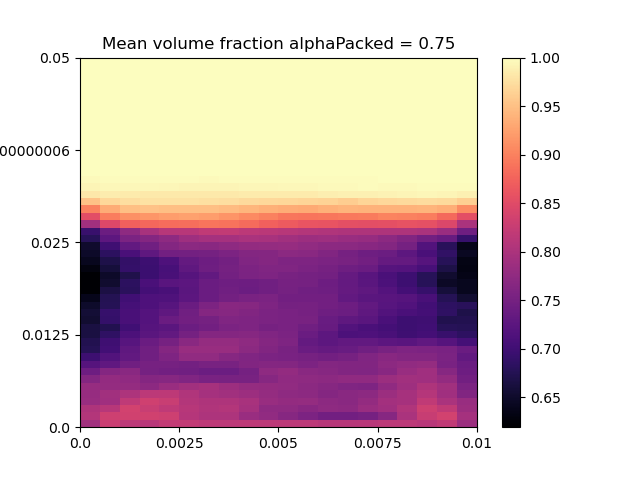
\includegraphics[width=0.9\linewidth]{sections/result/alphaPackedExp/2d_apacked_0.75_0.00005_0.07.png}
%     \caption{}
%     \label{fig:apackedExp3}
%     \end{subfigure}
%     \vspace{-0.15cm}
%     \begin{subfigure}[t]{0.49 \linewidth}
%     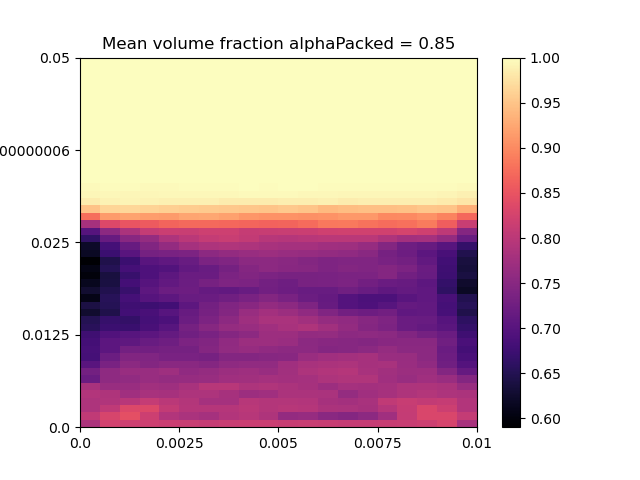
\includegraphics[width=0.9\linewidth]{sections/result/alphaPackedExp/2d_apacked_0.85_0.00005_0.07.png}
%     \caption{}
%     \label{fig:apackedExp4}
%     \end{subfigure}
%     \vspace{-0.15cm}
%     %\label{fig:placeholder}
% %\end{figure}
% %\FloatBarrier
% %\FloatBarrier
% %\begin{figure}
%     %\centering
%     \begin{subfigure}[t]{0.49 \linewidth}
%     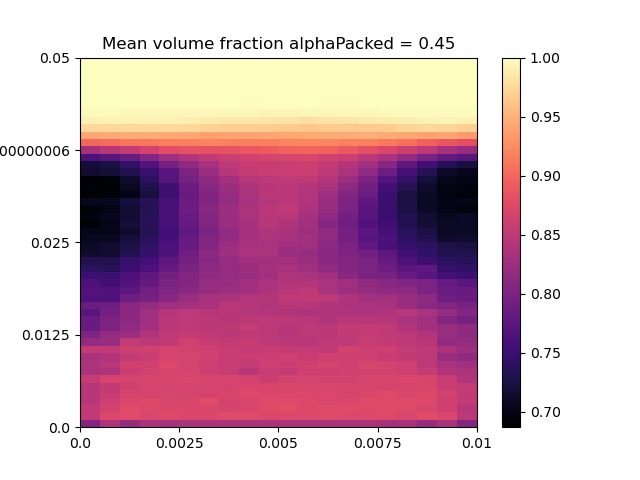
\includegraphics[width=0.9\linewidth]{sections/result/alphaPackedImp/2d_apacked_0.45_0.00005_0.07.png}
%     \caption{}
%     \label{fig:apackedImp1}
%     \end{subfigure}
%     \vspace{-0.15cm}
%     \begin{subfigure}[t]{0.49 \linewidth}
%     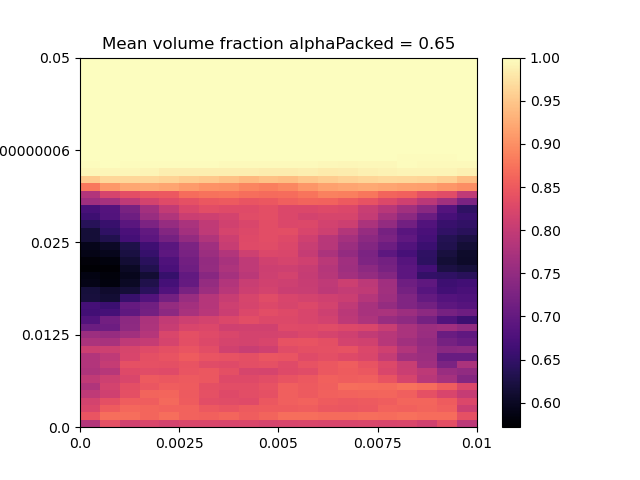
\includegraphics[width=0.9\linewidth]{sections/result/alphaPackedImp/2d_apacked_0.65_0.00005_0.07.png}
%     \caption{}
%     \label{fig:apackedImp2}
%     \end{subfigure}
%     % \end{figure}
%     % \begin{figure}\ContinuedFloat
%     \vspace{-0.15cm}
%     \begin{subfigure}[t]{0.49 \linewidth}
%     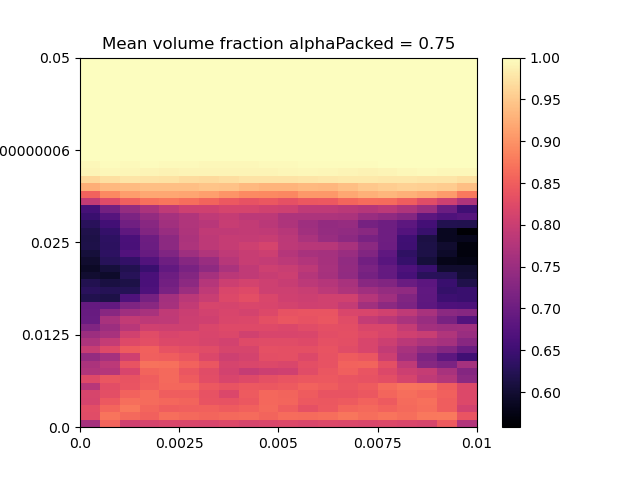
\includegraphics[width=0.9\linewidth]{sections/result/alphaPackedImp/2d_apacked_0.75_0.00005_0.07.png}
%     \caption{}
%     \label{fig:apackedImp3}
%     \end{subfigure}
%     \vspace{-0.15cm}
%     \begin{subfigure}[t]{0.49 \linewidth}
%     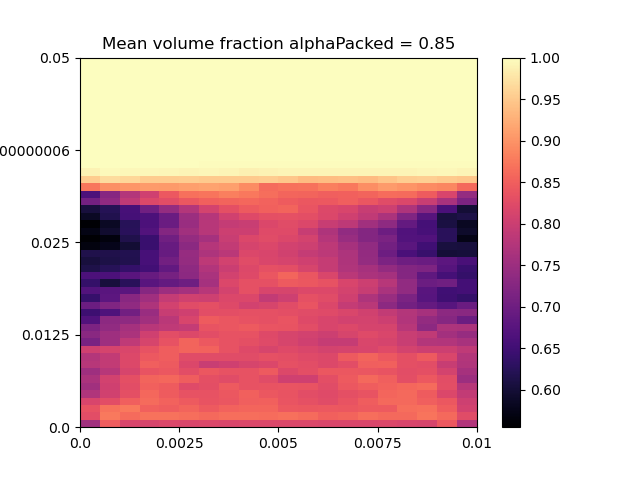
\includegraphics[width=0.9\linewidth]{sections/result/alphaPackedImp/2d_apacked_0.85_0.00005_0.07.png}
%     \caption{}
%     \label{fig:apackedImp4}
%     \end{subfigure}
%     \caption{Mean particle volume fraction for $0.5s - 5s$ for different values of $\pvfcp$. With packing model explicit (\ref{fig:apackedExp1}) - (\ref{fig:apackedExp4}) and implicit (\ref{fig:apackedImp1}) - (\ref{fig:apackedImp4}).}
%     \label{fig:aPacked}
% \end{figure}
% \FloatBarrier



\section{Damping Terms}
\subsection{Results collision damping}
\label{sec:DampResults}


We now include the collision damping term in the simulations. The term is not included in the standard \texttt{Goldschmidt} case.
We test the collision damping term in a total of $84$ cases:
\begin{table}[h!]
    \centering
    \begin{tabular}{ c | c | c}
         parameters & \texttt{OpenFOAM} & values \\
         \hline
         Damping type & \texttt{type} & \texttt{equilibrium}, \texttt{nonEquilibrium} \\
         Volume fraction, close packed $\pvfcp$ & \texttt{alphaPacked} & $0.5$, $0.6$, ,$0.65$, $0.7$, $0.8$, $0.9$ \\
         Restitution & \texttt{e} & $0.5$, $0.6$, $0.7$, $0.8$, $0.9$, $0.95$, $0.99$\\
    \end{tabular}
    %\caption{Parameters in the Goldschmidt tutorial with their \texttt{OpenFOAM} expression for the explicit and implicit packing model.}
    \label{tab:placeholder}
\end{table}

Simulations are run with an adjustable time step limited by a Courant number of $0.6$. Simulations are terminated if the calculation time of single time step takes longer than ten minutes or the time step falls below a threshold of $10^{-20}s$.
The final simulation times are listed in the two tables below for the non-equilibrium and the equilibrium term.


\begin{table}[h!]
    \centering
    \begin{tabular}{|l|*{7}{c|}}\hline
\backslashbox{$\pvfcp$}{\texttt{e}}
& 0.5 & 0.6 & 0.7 & 0.8 & 0.9 & 0.95 & 0.99 \\ \hline
0.5&
0.040972 &
0.008742&
0.018896&
0.008541&
0.007831&
0.008786&
0.007331 \\ \hline
0.65 &
0.22957&
0.336456&
0.497744&
0.350028&
0.660727&
1.05699&
1.01343
\\ \hline
0.6 &
0.529419&
0.795894&
0.728319&
1.459815&
0.584578&
0.851135&
0.611465\\ \hline
0.7  &
0.640304&
1.103907&
0.789877&
1.03854&
0.586462&
0.423384&
0.909999\\ \hline
0.8 &
0.866482 &
0.466389&
1.544282&
0.928576&
2.834396&
2.450749&
0.550631 \\ \hline
0.9  &
0.483467&
0.589252&
2.029631&
2.889477&
3.018472&
1.529281&
\cellcolor{ForestGreen!33}4.999988
\\ \hline
\end{tabular}    
    \caption{Runtime for the damping term type \texttt{equilibrium} rounded. Entries marked in green reached a simulation time of $5$ seconds.}
    \label{tab:placeholder}
\end{table}

\begin{table}[h!]
    \centering
    \begin{tabular}{|l|*{7}{c|}}\hline
\backslashbox{$\pvfcp$}{\texttt{e}}
& 0.5 & 0.6 & 0.7 & 0.8 & 0.9 & 0.95 & 0.99 \\ \hline
0.5&
0.010063&
0.014112&
0.012930&
0.013440&
0.009998&
0.005540&
0.009905
\\ \hline
0.6 &
0.345276&
0.36796&
0.586591&
0.655485&
0.670003&
0.575027&
0.091037
\\ \hline
0.65 &
0.801246&
1.09722&
0.578553&
1.014649&
0.585877&
0.804848&
0.537676
\\ \hline
0.7 &
0.885873 &
1.490554 &
0.647732 &
0.611606&
0.573212&
1.102617&
1.363100 
\\ \hline
0.8 &
2.245529&
2.700315&
2.526333&
1.0928&
1.813442&
1.812381&
0.746165
\\ \hline
0.9  &
0.777422 &
\cellcolor{ForestGreen!33}5.000106 &
2.247512&
2.109448&
1.328963&
3.339160&
2.888154
\\ \hline
\end{tabular}    
    \caption{Runtime for the damping term type \texttt{nonEquilibrium}. Entries marked in green reached a simulation time of $5$ seconds.}
    \label{tab:placeholder}
\end{table}

Out of the $84$ cases two terms reached a simulation time of five seconds. The term is therefore not considered in further applications.

\subsection{Results return-to-isotropy}
The second damping term modifies the particle velocities based on a velocity distribution to imitate the scattering from collisions and is described in detail in sec \ref{sec:MPLoop}.
To conserve comparability the seed which we use to draw from velocity distributions is fixed to $123456$.
We run the simulation with a random seed a total of fifty times.
For a total of $1000$ we save the fluid volume fraction and calculate a mean value for each sample point.
We then calculate the maximal distance from the mean for each time step.
The result can be observed in figure \ref{fig:maxDiffIso}.

\begin{figure}[h!]
    \centering
    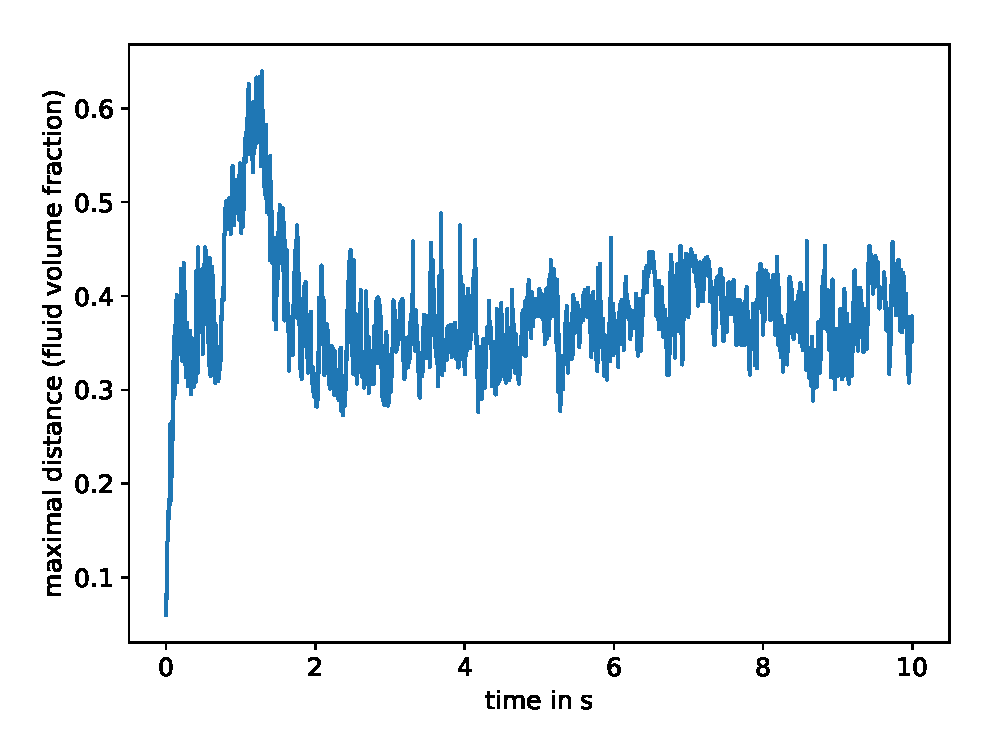
\includegraphics[width=0.6\linewidth]{sections/result/isotropyModel.eps}
    \caption{Maximal difference of fluid volume to the mean fluid volume fraction in $1000$ points.}
    \label{fig:maxDiffIso}
\end{figure}

After the particles first fall down the maximal difference to the mean error spikes to over $0.6$.
In the following figure \ref{fig:diffIsoPV} two cases at time step $0.999741$ and $0.999599$ are depicted.
In one case the fluid forms a layer in between the particles while in the second it does not.
This leads to a large local difference in the fluid volume fraction.
%nr 0

\begin{figure}[h!]
    \centering
    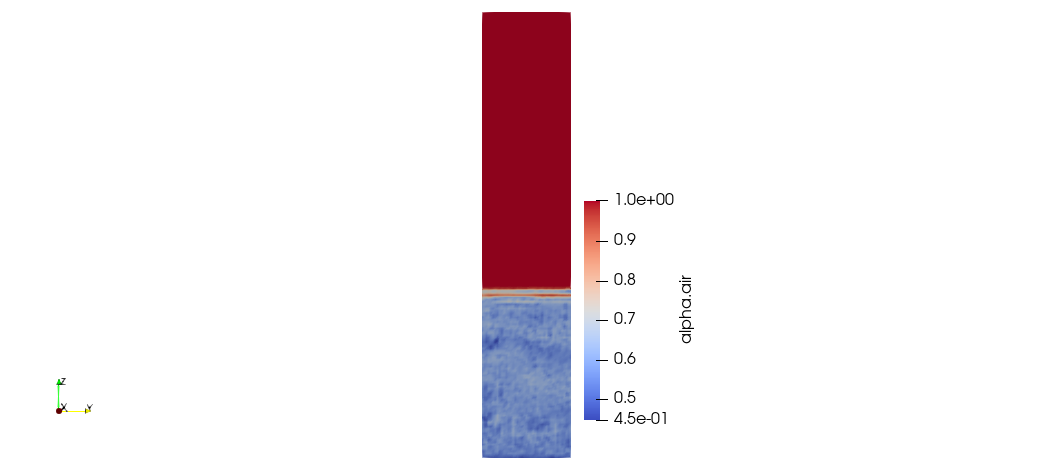
\includegraphics[height =5.5cm, trim = {10cm 0 10cm 0},clip]{sections/result/Part_wrong_iso.png}
    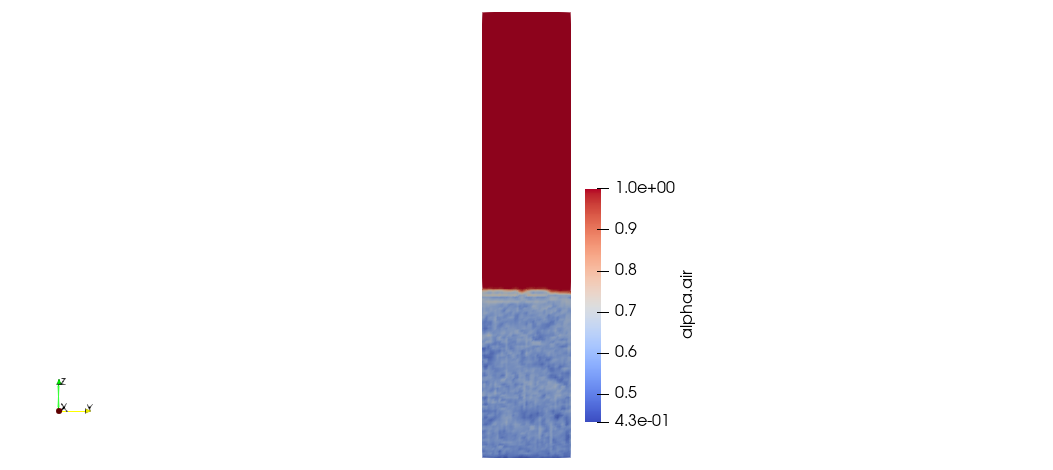
\includegraphics[height = 5.5cm, trim = {10cm 0 10cm 0},clip]{sections/result/no_line_iso.png}
    \caption{Fluid volume fraction for two different seeds at $t = 0.999741$ (left) and $t = 0.999599$ (right).}
    \label{fig:diffIsoPV}
\end{figure}
In the following we use again use a fixed seed for the simulations.

% \begin{figure}[h!]
% \captionsetup[subfigure]{
%   font={footnotesize},
%   %justification=raggedright,
%   singlelinecheck=false,
%   position=below,
%   %aboveskip=2.5cm, %belowskip=2.5cm,
%   skip=-0.9cm
%   %margin={0cm,-1cm}
% }
%     \centering
%     \vspace{-0.2cm}
%     \begin{subfigure}[t]{0.49 \linewidth}
%     %\caption{} 
%     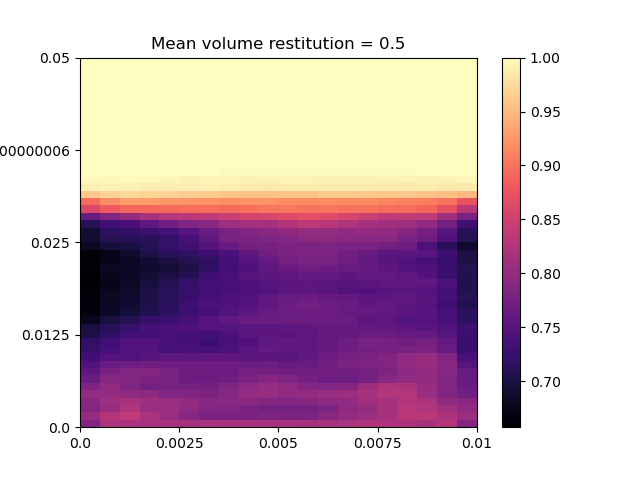
\includegraphics[width=0.9\linewidth]{sections/result/IsotropyExp/2d_apacked_0.5_0.65_0.00005_0.07.png}
%     \caption{}
%     \label{fig:IsotropyExp1}
%     \end{subfigure}
%     \vspace{-0.2cm}
%     \begin{subfigure}[t]{0.49 \linewidth}
%     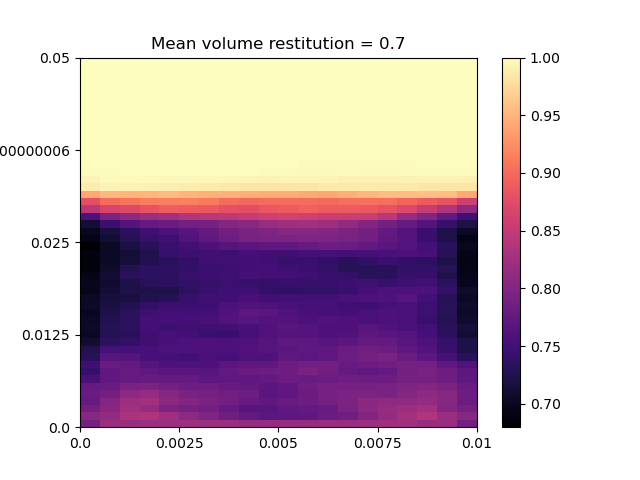
\includegraphics[width=0.9\linewidth]{sections/result/IsotropyExp/2d_apacked_0.7_0.65_0.00005_0.07.png}
%     \caption{}
%     \label{fig:IsotropyExp2}
%     \end{subfigure}
%     \vspace{-0.15cm}
%     \begin{subfigure}[t]{0.49 \linewidth}
%     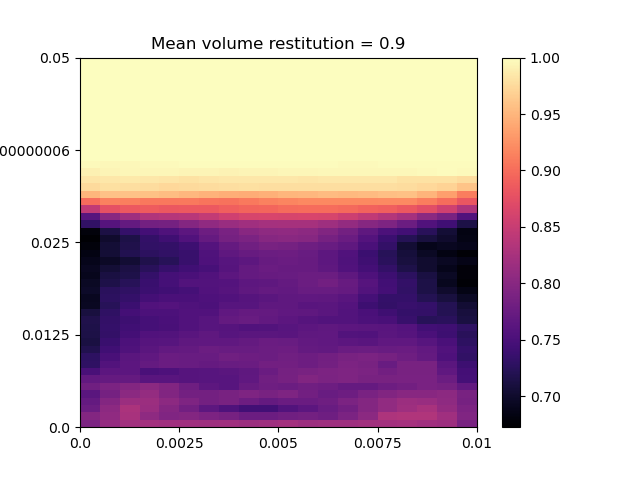
\includegraphics[width=0.9\linewidth]{sections/result/IsotropyExp/2d_apacked_0.9_0.65_0.00005_0.07.png}
%     \caption{}
%     \label{fig:IsotropyExp3}
%     \end{subfigure}
%     \vspace{-0.15cm}
%     \begin{subfigure}[t]{0.49 \linewidth}
%     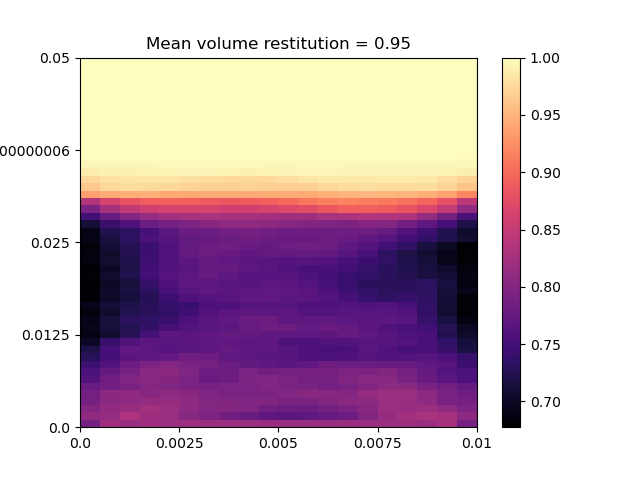
\includegraphics[width=0.9\linewidth]{sections/result/IsotropyExp/2d_apacked_0.95_0.65_0.00005_0.07.png}
%     \caption{}
%     \label{fig:IsotropyExp4}
%     \end{subfigure}
%     \vspace{-0.15cm}
%     %\label{fig:placeholder}
% %\end{figure}
% %\FloatBarrier
% %\FloatBarrier
% %\begin{figure}
%     %\centering
%     \begin{subfigure}[t]{0.49 \linewidth}
%     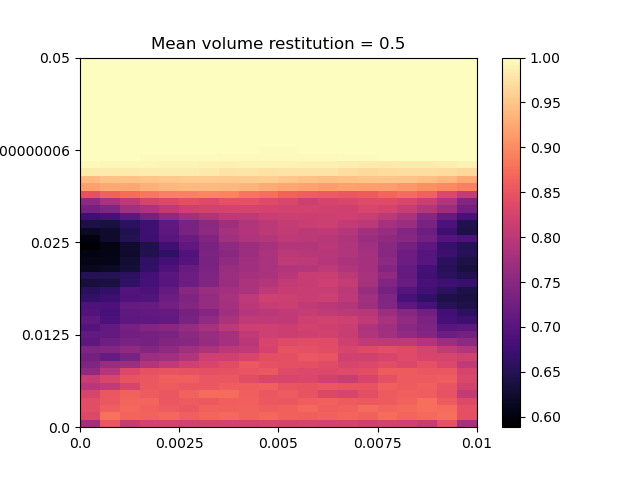
\includegraphics[width=0.9\linewidth]{sections/result/IsotropyImp/2d_apacked_0.5_0.65_0.00005_0.07.png}
%     \caption{}
%     \label{fig:IsotropyImp1}
%     \end{subfigure}
%     \vspace{-0.15cm}
%     \begin{subfigure}[t]{0.49 \linewidth}
%     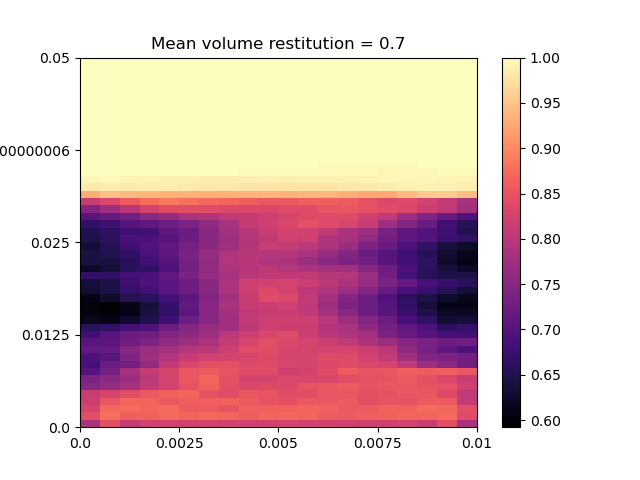
\includegraphics[width=0.9\linewidth]{sections/result/IsotropyImp/2d_apacked_0.7_0.65_0.00005_0.07.png}
%     \caption{}
%     \label{fig:IsotropyImp2}
%     \end{subfigure}
%     \end{figure}
%     \begin{figure}[h!]\ContinuedFloat
%     \centering
%     \begin{subfigure}[t]{0.49 \linewidth}
%     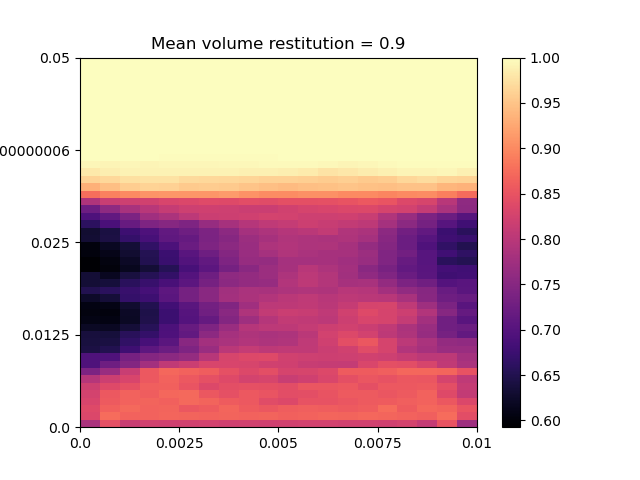
\includegraphics[width=0.9\linewidth]{sections/result/IsotropyImp/2d_apacked_0.9_0.65_0.00005_0.07.png}
%     \caption{}
%     \label{fig:IsotropyImp3}
%     \end{subfigure}
%     \vspace{-0.15cm}
%     \begin{subfigure}[t]{0.49 \linewidth}
%     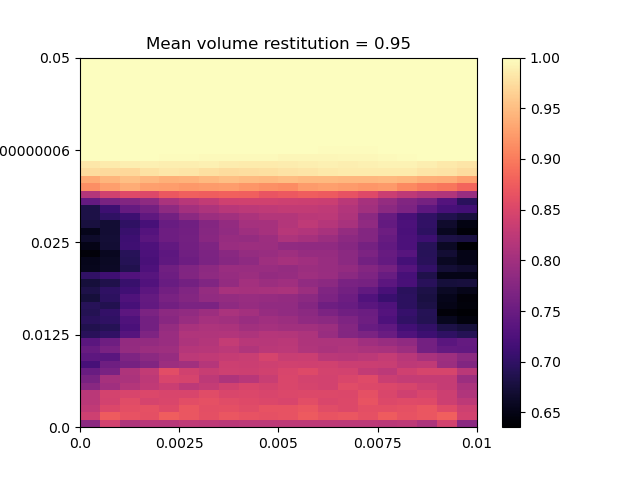
\includegraphics[width=0.9\linewidth]{sections/result/IsotropyImp/2d_apacked_0.95_0.65_0.00005_0.07.png}
%     \caption{}
%     \label{fig:IsotropyImp4}
%     \end{subfigure}
%     \caption{Mean particle volume fraction for $0.5s - 5s$ for different values of $e_p$. With packing model explicit (\ref{fig:IsotropyExp1}) - (\ref{fig:IsotropyExp4}) and implicit (\ref{fig:IsotropyImp1}) - (\ref{fig:IsotropyImp4}).}
%     \label{fig:Isotropy}
% \end{figure}
%  \FloatBarrier


% \subsection{Drag Model}
% The frictional pressure drop was empirically correlated to the cube Reynolds number
% \begin{equation*}
%     F_D = (A \pvf + B \operatorname{Re}_p) \dfrac{\pvf \mu_f}{\fvf^2 d_p^2} \qquad \operatorname{Re}_p = \dfrac{\rf \lvert \u_{rel} \rvert d_p}{\mu_f}
% \end{equation*}
% Several different coefficient values have been proposed for $A$ and $B$. %\Todo{Ein paar schreiben}
% Two models available in \OF are the Plessis-Masliyah drag model \cite{Plessis}
% \begin{equation*}
%     A = \dfrac{26.8 \fvf^2}{\pvf^{2/3}(1-\pvf^{1/3})(1-\fvf^{2/3}} \qquad B = \dfrac{\fvf^2}{(1-\pvf^{2/3})^2}
% \end{equation*}
% and the Ergun-Wen-Yu model \cite{ErgunWenYu}
% \begin{equation*}
%     F_D = \begin{cases}
%         \dfrac{3 (1-\fvf) \mu_f \fvf \operatorname{Re}_p}{d_p^2} C_D \fvf^{-2.65} & \text{if } \fvf \geq 0.8 \\
%         \left(150 \dfrac{1-\fvf}{\fvf} + 1.75 \operatorname{Re}_p \right) \dfrac{(1-\fvf) \mu_f}{d_p^2} & \text{if } \fvf < 0.8
%     \end{cases} \qquad C_D = \begin{cases}
%         24 \left(1+0.15 \operatorname{Re}_p^{0.687}\right) & \text{if } \operatorname{Re}_p < 1000 \\
%         0.44 & \text{if } \operatorname{Re}_p \geq 1000
%     \end{cases}
% \end{equation*}
% which uses the Ergun expression for fluid volume fractions below $0.8$ .

% \section{Pressure drop}
% %\Todo{Plot einfügen}
% At the beginning of this thesis in the background chapter we discussed the pressure drop in a fluidized bed reactor, see section \ref{sec:basicFBR}.
% We expect the pressure drop grows linearly at first. 
% As we reach the minimum fluidization velocity we expect to get a slight increase in pressure drop before staying nearly constant in order to match the experimental data.

% We can observe that behavior in the following plot
% \begin{figure}[h!]
%     \centering
%     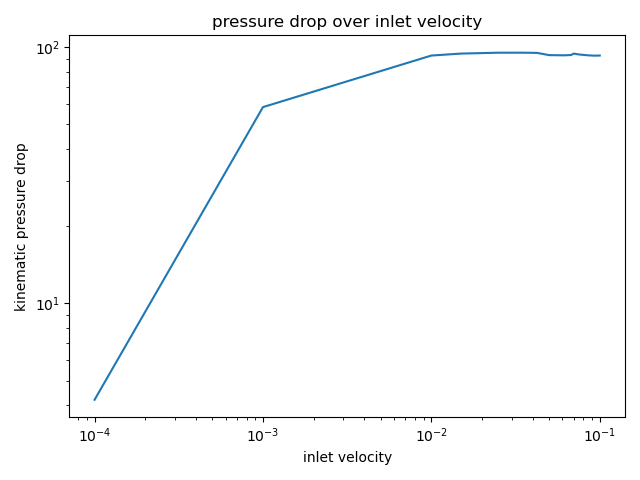
\includegraphics[width=0.5\linewidth]{sections/result/pressureDrop.png}
%     \caption{Kinematic pressure drop}
%     \label{fig:placeholder}
% \end{figure}




\section{Parameter Study}
\label{sec:paramStudy}
To fit our simulation to the given data we vary the models and parameters of the \MP method. The particle normal stress, here chosen as the explicit Harris and Crighton model, depends on the particle close pack volume fraction $\pvfcp$, the exponent $\beta$ and the pressure constant $P_s$. As all three have different influences on the simulation we always vary two parameters at a time and leave the third as defined in the \lstinline|Goldschmidt| tutorial, see table \ref{tab:cases},
% \begin{table}[h!]
%     \centering
%     \begin{tabular}{c|c c c}
%         Parameters & $\pvfcp$ & $\beta$ & $P_s$ \\
%         \hline
%         Case 1  & \lstinline|0.55|, \lstinline|0.58|, \lstinline|0.6|, \lstinline|0.63|, \lstinline|0.65|, \lstinline|0.68|, \lstinline|0.7| & \lstinline|1.5|, \lstinline|2.0|, \lstinline|2.5|, \lstinline|3.0|, \lstinline|3.5|, \lstinline|4.0|, \lstinline|4.5|, \lstinline|5.0| & \lstinline|10.0|\\
%         Case 2 & \lstinline|0.55|, \lstinline|0.58|, \lstinline|0.6|, \lstinline|0.63|, \lstinline|0.65|, \lstinline|0.68|, \lstinline|0.7| & \lstinline|2.0| & \lstinline|5.0|, \lstinline|6.0|, \lstinline|7.0|, \lstinline|8.0|, \lstinline|9.0|, \lstinline|10.0|\\
%         Case 3 & \lstinline|0.65| & \lstinline|1.5|, \lstinline|2.0|, \lstinline|2.5|, \lstinline|3.0|, \lstinline|3.5|, \lstinline|4.0|, \lstinline|4.5|, \lstinline|5.0| & \lstinline|5.0|, \lstinline|6.0|, \lstinline|7.0|, \lstinline|8.0|, \lstinline|9.0|, \lstinline|10.0|
%     \end{tabular}
%     \caption{Caption}
%     \label{tab:placeholder}
% \end{table}

\begin{table}[h!]
    \centering
    \begin{tabular}{c|c c c}
        Parameters & $\pvfcp$ & $\beta$ & $P_s$ \\
        \hline
        Case 1  &  $ \pvfcp \in [0.55 , 0.7]$ & $\beta \in [1.5 , 5.0]$ & $P_s = 10.0$ \\
        %\lstinline|0.55|, \lstinline|0.58|, \lstinline|0.6|, \lstinline|0.63|, \lstinline|0.65|, \lstinline|0.68|, \lstinline|0.7| & \lstinline|1.5|, \lstinline|2.0|, \lstinline|2.5|, \lstinline|3.0|, \lstinline|3.5|, \lstinline|4.0|, \lstinline|4.5|, \lstinline|5.0| & \lstinline|10.0|\\
        Case 2 & $\pvfcp \in [0.55,0.7]$ & $\beta = 2.0$ & $P_s \in [5.0,10.0]$ \\
        %\lstinline|0.55|, \lstinline|0.58|, \lstinline|0.6|, \lstinline|0.63|, \lstinline|0.65|, \lstinline|0.68|, \lstinline|0.7| & \lstinline|2.0| & \lstinline|5.0|, \lstinline|6.0|, \lstinline|7.0|, \lstinline|8.0|, \lstinline|9.0|, \lstinline|10.0|\\
        Case 3 & $\pvfcp =0.65$ & $\beta \in [1.5 , 5.0]$ & $P_s \in [5.0,10.0]$
        %\lstinline|0.65| & \lstinline|1.5|, \lstinline|2.0|, \lstinline|2.5|, \lstinline|3.0|, \lstinline|3.5|, \lstinline|4.0|, \lstinline|4.5|, \lstinline|5.0| & \lstinline|5.0|, \lstinline|6.0|, \lstinline|7.0|, \lstinline|8.0|, \lstinline|9.0|, \lstinline|10.0|
    \end{tabular}
    \caption{Caption}
    \label{tab:cases}
\end{table}
with exact parameters as listed in table \ref{tab:exact_param}.
\begin{table}[h!]
    \centering
    \begin{tabular}{c|c}
    Parameter & Values \\
    \hline
     $\pvfcp$ & \lstinline|0.55|, \lstinline|0.58|, \lstinline|0.6|, \lstinline|0.63|, \lstinline|0.65|, \lstinline|0.68|, \lstinline|0.7| \\
     $\beta $ & \lstinline|1.5|, \lstinline|2.0|, \lstinline|2.5|, \lstinline|3.0|, \lstinline|3.5|, \lstinline|4.0|, \lstinline|4.5|, \lstinline|5.0| \\
     $P_s$ & \lstinline|5.0|, \lstinline|6.0|, \lstinline|7.0|, \lstinline|8.0|, \lstinline|9.0|, \lstinline|10.0|
\end{tabular}
    \caption{Parameters for the Harris and Crighton model}
    \label{tab:exact_param}
\end{table}
% For the close pack volume fraction we use the parameters $\pvfcp$ = \{ \lstinline|0.55|, \lstinline|0.58|, \lstinline|0.6|, \lstinline|0.63|, \lstinline|0.65|, \lstinline|0.68|, \lstinline|0.7|\} the exponent as $\beta $= \{\lstinline|1.5|, \lstinline|2.0|, \lstinline|2.5|, \lstinline|3.0|, \lstinline|3.5|, \lstinline|4.0|, \lstinline|4.5|, \lstinline|5.0|\} and the pressure constant as $P_s$ = \{\lstinline|5.0|, \lstinline|6.0|, \lstinline|7.0|, \lstinline|8.0|, \lstinline|9.0|, \lstinline|10.0|\}.


% \begin{table}[h!]
%     \centering
%     \begin{tabular}{c|c c c}
%         Parameters & Case 1 & Case 2 & Case 3 \\
%         $\pvfcp$ & \lstinline|0.55|, \lstinline|0.58|, \lstinline|0.6|, \lstinline|0.63|, \lstinline|0.65|, \lstinline|0.68|, \lstinline|0.7|& \lstinline|0.55|, \lstinline|0.58|, \lstinline|0.6|, \lstinline|0.63|, \lstinline|0.65|, \lstinline|0.68|, \lstinline|0.7|& \lstinline|0.65| \\
%         $\beta$ & \lstinline|1.5|, \lstinline|2.0|, \lstinline|2.5|, \lstinline|3.0|, \lstinline|3.5|, \lstinline|4.0|, \lstinline|4.5|, \lstinline|5.0|&\lstinline|2.0| & \lstinline|1.5|, \lstinline|2.0|, \lstinline|2.5|, \lstinline|3.0|, \lstinline|3.5|, \lstinline|4.0|, \lstinline|4.5|, \lstinline|5.0| \\
%         $P_s$ & \lstinline|10.0| & \lstinline|5.0|, \lstinline|6.0|, \lstinline|7.0|, \lstinline|8.0|, \lstinline|9.0|, \lstinline|10.0| & \lstinline|5.0|, \lstinline|6.0|, \lstinline|7.0|, \lstinline|8.0|, \lstinline|9.0|, \lstinline|10.0|
%     \end{tabular}
% \end{table}
% \begin{table}[h!]
%     \centering
%     \begin{tabular}{c|c c c}    
%         Parameters & $\pvfcp$ & $\beta$ & $P_s$ \\
%         \hline
%         Case 1  & \lstinline|0.55|, \lstinline|0.58|, \lstinline|0.6|, \lstinline|0.63|, \lstinline|0.65|, \lstinline|0.68|, \lstinline|0.7| & \lstinline|1.5|, \lstinline|2.0|, \lstinline|2.5|, \lstinline|3.0|, \lstinline|3.5|, \lstinline|4.0|, \lstinline|4.5|, \lstinline|5.0| & \lstinline|10.0|\\
%         Case 2 & \lstinline|0.55|, \lstinline|0.58|, \lstinline|0.6|, \lstinline|0.63|, \lstinline|0.65|, \lstinline|0.68|, \lstinline|0.7| & \lstinline|2.0| & \lstinline|5.0|, \lstinline|6.0|, \lstinline|7.0|, \lstinline|8.0|, \lstinline|9.0|, \lstinline|10.0|\\
%         Case 3 & \lstinline|0.65| & \lstinline|1.5|, \lstinline|2.0|, \lstinline|2.5|, \lstinline|3.0|, \lstinline|3.5|, \lstinline|4.0|, \lstinline|4.5|, \lstinline|5.0| & \lstinline|5.0|, \lstinline|6.0|, \lstinline|7.0|, \lstinline|8.0|, \lstinline|9.0|, \lstinline|10.0|
%     \end{tabular}
%     \caption{Caption}
%     \label{tab:placeholder}
% \end{table}
Apart from the Harris and Crighton model, the drag model is varied, the isotropy model is switched on and off, and four different inlet velocities are considered. 
\begin{table}[h!]
    \centering
    \begin{tabular}{c|c c c c}
         drag &  \lstinline|ErgunWenYu| & \lstinline|PlessisMaliyahDrag|& &\\
         isotropy & \lstinline|stochastic| & \lstinline|none| & & \\
         velocity & 0.015 & 0.025 & 0.034 & 0.042
    \end{tabular}
    \caption{Sixteen cases are tested with different parameters for $\pvfcp$, $\beta$, $P_s$}
    \label{tab:placeholder}
\end{table}

The velocities are selected to ensure that the bed is in a fluidized state.
In a fluidized state the mean bed height varies only slightly. 
From the provided images we can deduce a mean bed height, see \ref{fig:bed_height_exp} and choose velocities so the volumetric inflow rate is between $0.07 \operatorname{l}/\operatorname{min}$ and $0.2 \operatorname{l}/\operatorname{min}$.

The bed height is gathered from the provided images.
We crop the pixel to only include the tube of the fluidized bed reactor, see \ref{fig:img_processing}.
We iterate over the pixels in one column starting from the top.
We start at the first pixel with a light difference of zero.
The pixel is updated if the light difference of the pixel considered with the one below it is higher than the current light difference.
To make sure we enter a bed instead of leaving it we check if we have a negative difference, because the bed is white and therefor brighter and if the pixel below has a value of at least $120$ to check we are in a bed and not at a smudge.
We average over the columns and take the result as the bed height
\begin{figure}
    \centering
    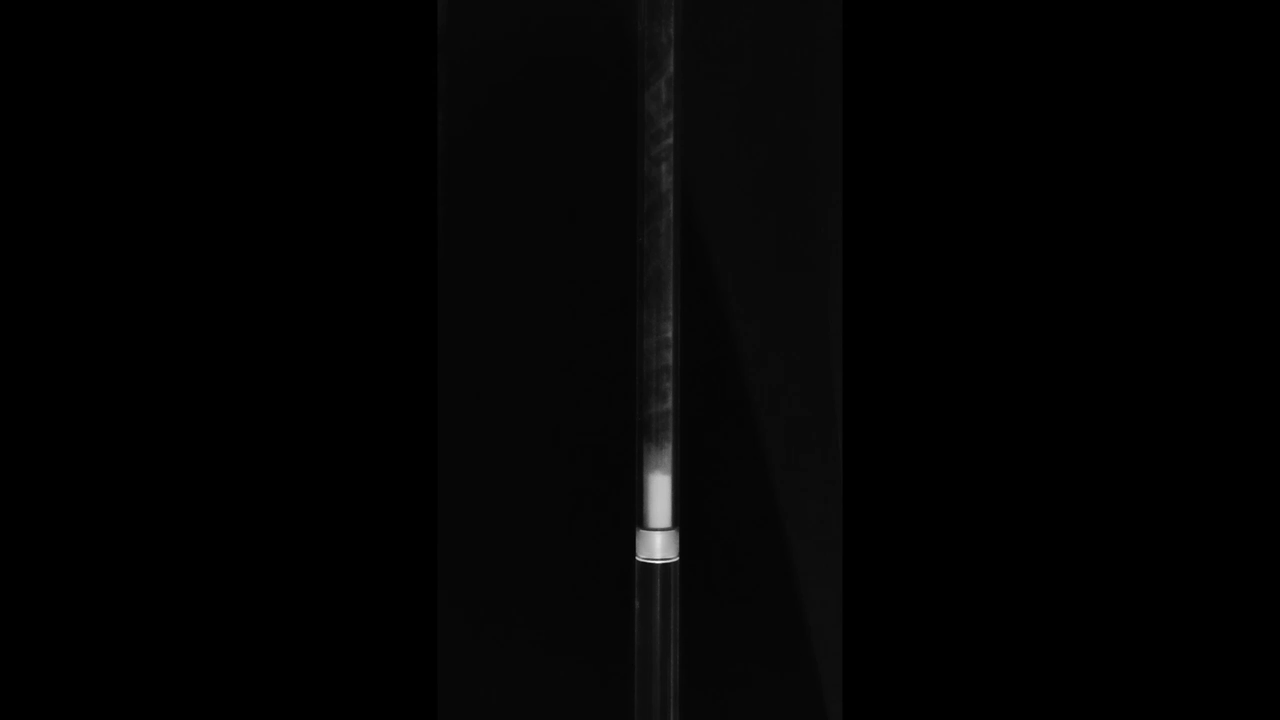
\includegraphics[width = 0.395 \linewidth, trim = {12cm 0 12cm 0},clip]{sections/result/016_grey19.png}
    \hspace{4cm}
    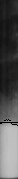
\includegraphics[width=0.048\linewidth]{sections/result/016_crop19.png}
    \caption{Image processing for bed height for a single time step at velocity $\uf = 0.034 m/s$. On the left images of the fluidized bed reactor provided by. On the right hand side the bed height. The single dots represent the bed height of the column. The solid line represents the mean bed height.}
    \label{fig:img_processing}
\end{figure}
The bed height over the velocity is presented in the following figure \ref{fig:bed_height_exp}.
\begin{figure}[h!]
    \centering
    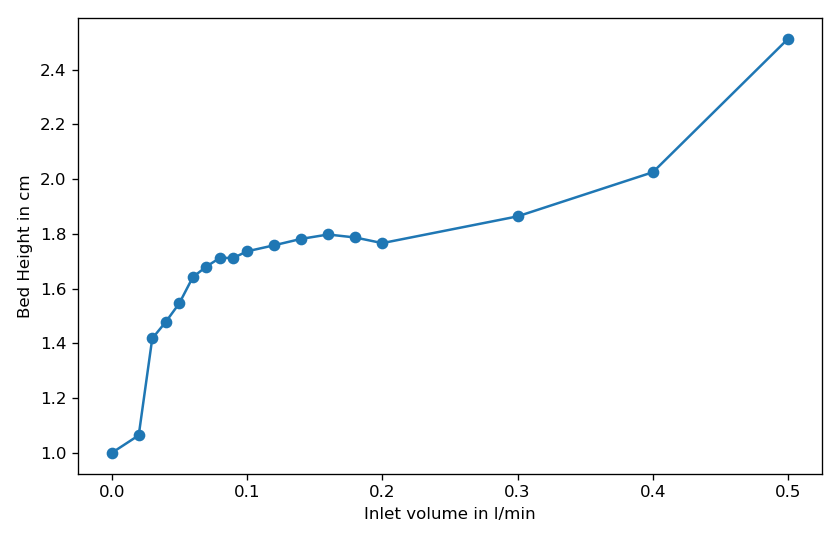
\includegraphics[width=0.7\linewidth]{sections/result/expBedHeightWobble.png}
    \caption{Caption}
    \label{fig:bed_height_exp}
\end{figure}


The aim of this section is to fit simulation parameters of different inlet velocities to the data provided by the experiments listed in table \ref{tab:expData}.
\begin{table}[h!]
    \centering
    \begin{tabular}{c|c c c}
         volumetric flow rate (l/min) & velocity (m/s) & pressure drop (Pa) & bed height (cm) \\
         \hline
         0.07 & 0.015 & 140 & 1.68\\
         0.12 & 0.025 & 149 & 1.76\\
         0.16 & 0.034 & 157 & 1.80\\
         0.2 & 0.042 & 159 & 1.76 
    \end{tabular}
    \caption{Bed height for different volumetric flow rates.}
    \label{tab:expData}
\end{table}
The provided data consists of a mean pressure drop and a mean bed height.
Fitting parameters is done by minimizing the relative error for the data
 \begin{equation}
 \label{eq:relError}
        err = \sqrt{\left( \dfrac{\Delta p - \Delta p_{exp}}{\Delta p_{exp}}\right)^2 + \left( \dfrac{h_{bed} - h_{bed,exp}}{h_{bed,exp}} \right)^2}.
\end{equation}


\ifschonwars
\subsection{Case 1: $\pvfcp$ and $\beta$}
%first pressure, second height, third both
In this section we look at the first case where the close pack volume fraction $\pvfcp$ and the exponent $\beta$ are varied. The pressure constant $P_s$ is left constant.
We test the parameters for four inlet velocities.

\subsubsection{Inlet velocity $\uf = 0.015m/s$}
For an inlet velocity $\uf = 0.015m/s$ we expect a bed height of $1.68cm$ and a pressure drop of $140 Pa$

\paragraph{Drag model \lstinline|ErgunWenYu| and isotropy model \lstinline|none|}

\FloatBarrier
\begin{figure}[h!]
    \centering
    \begin{subfigure}[b]{0.49 \linewidth}
        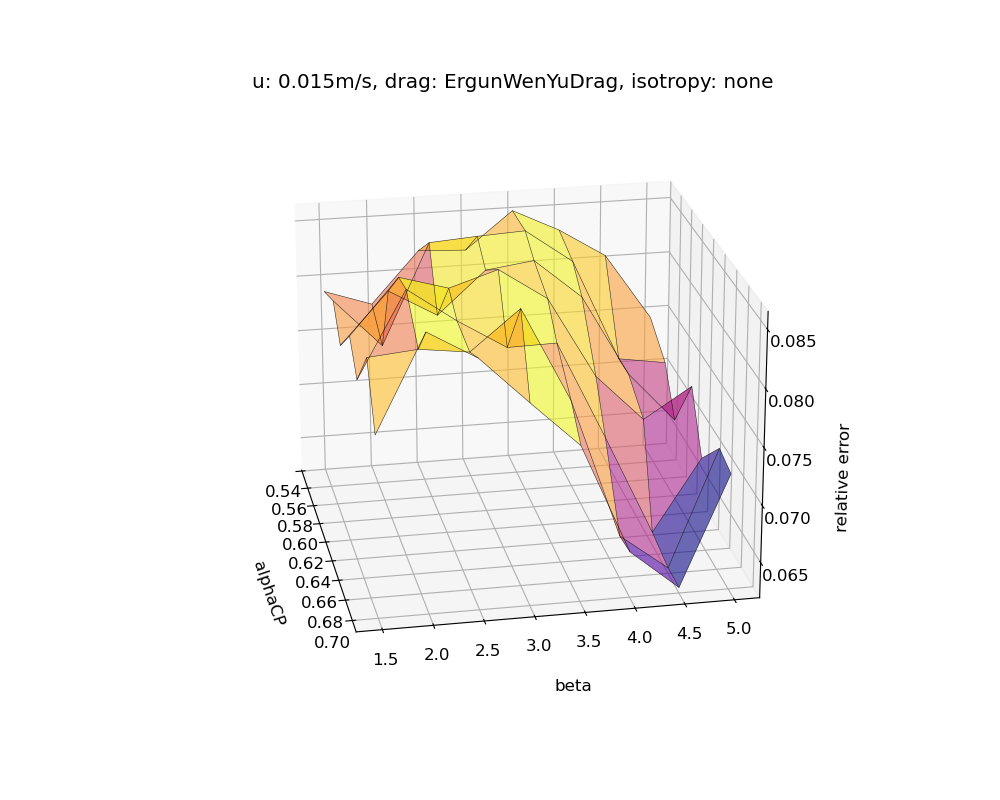
\includegraphics[width = \linewidth, trim = {3.5cm 0 3.5cm 0}, clip]{sections/result/Case 1/Z_pres0.015_ErgunWenYuDrag_none.png}
        \caption{Relative error of pressure with drag model \lstinline|ErgunWenYuDrag|, isotropy model \lstinline|none| and inlet velocity $0.015m/s$.}
    \end{subfigure}
    \hfill
    \begin{subfigure}[b]{0.49 \linewidth}
        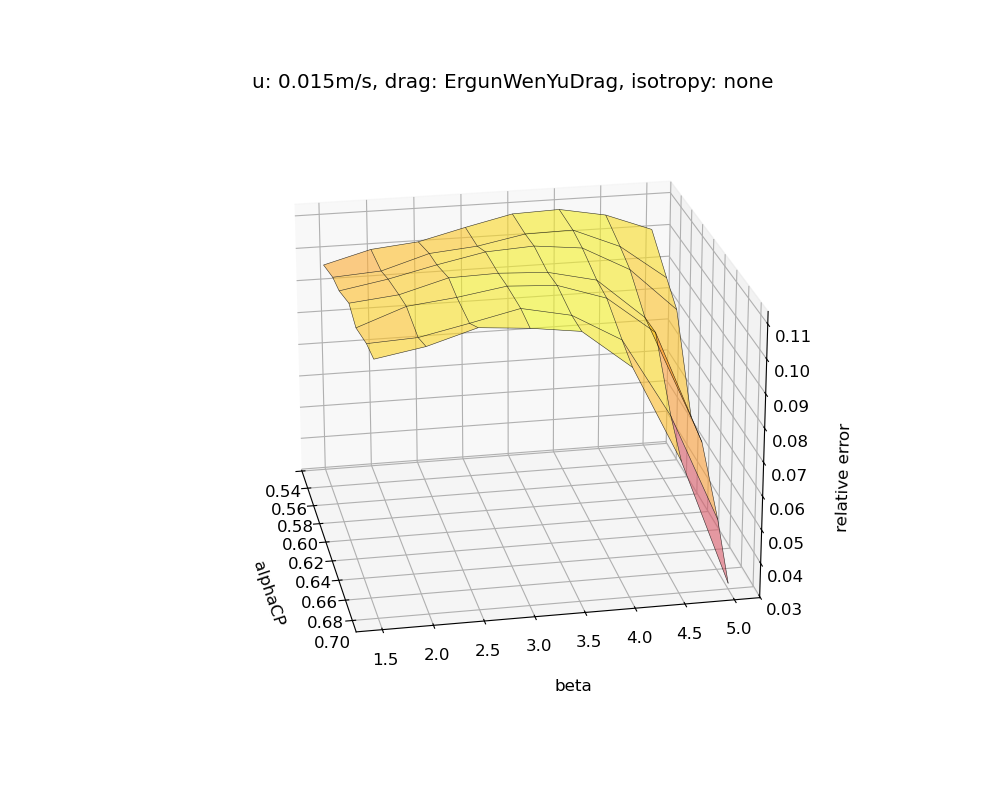
\includegraphics[width = \linewidth, trim = {3.5cm 0 3.5cm 0}, clip]{sections/result/Case 1/Z_heightZ_pres0.015_ErgunWenYuDrag_none.png}
        \caption{Relative error of bed height with drag model \lstinline|ErgunWenYuDrag|, isotropy model \lstinline|none| and inlet velocity $0.015m/s$.}
    \end{subfigure}
\end{figure}

\begin{figure}[h!]
    \centering
    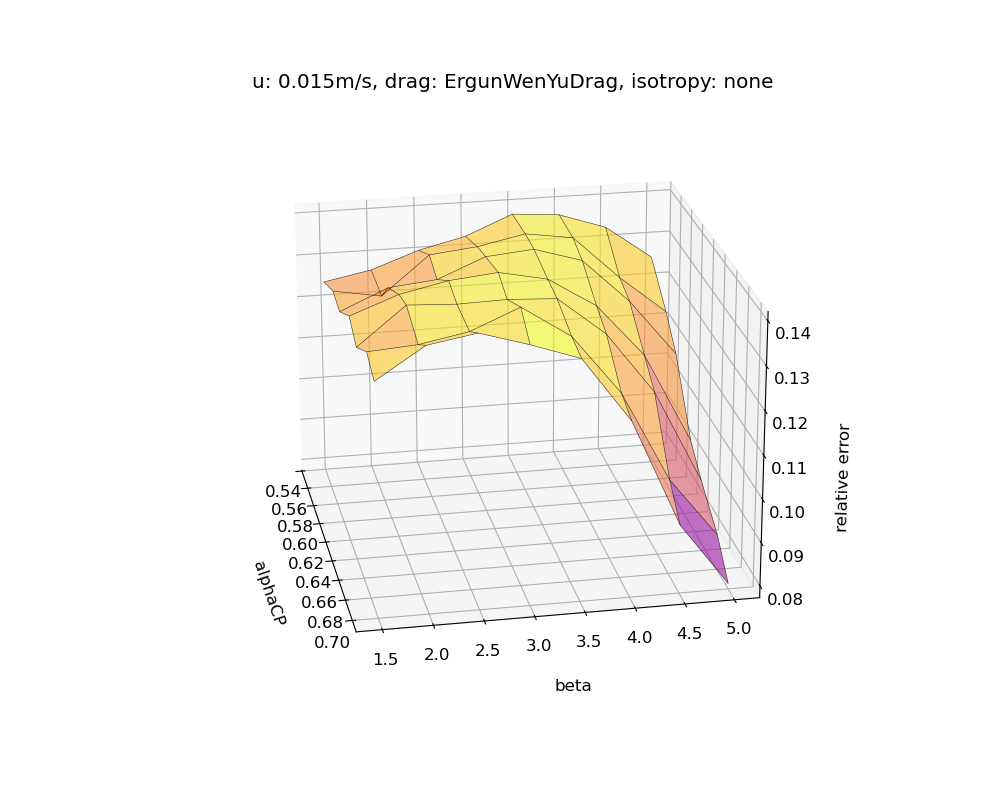
\includegraphics[width=0.5\linewidth, trim = {3.5cm 0 3.5cm 0}, clip]{sections/result/Case 1/Z_bothZ_heightZ_pres0.015_ErgunWenYuDrag_none.png}
    \caption{Combined relative error with drag model \lstinline|ErgunWenYuDrag|, isotropy model \lstinline|none| and inlet velocity $0.015m/s$, according to equation \eqref{eq:relError}.}
    \label{fig:placeholder}
\end{figure}
\FloatBarrier




\paragraph{Drag model \lstinline|ErgunWenYu| and isotropy model \lstinline|stochastic|}
\FloatBarrier
\begin{figure}[h!]
    \centering
    \begin{subfigure}[b]{0.49 \linewidth}
        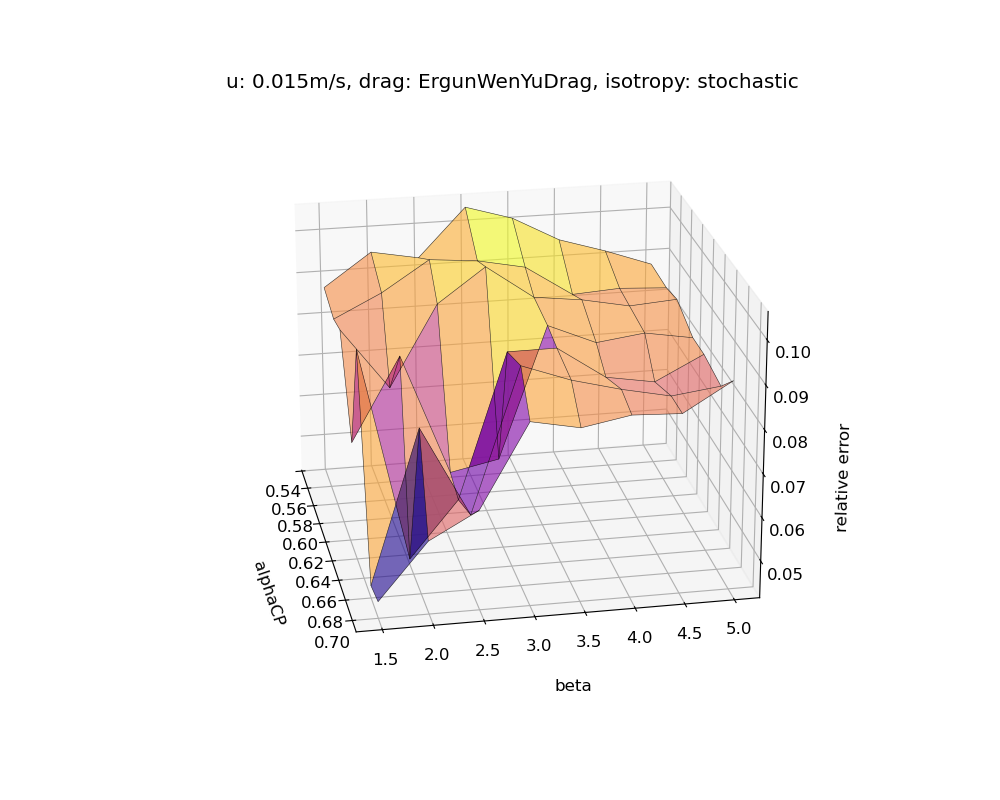
\includegraphics[width = \linewidth, trim = {3.5cm 0 3.5cm 0}, clip]{sections/result/Case 1/Z_pres0.015_ErgunWenYuDrag_stochastic.png}
        \caption{Relative error of pressure with drag model \lstinline|ErgunWenYuDrag|, isotropy model \lstinline|stochastic| and inlet velocity $0.015m/s$.}
    \end{subfigure}
    \hfill
    \begin{subfigure}[b]{0.49 \linewidth}
        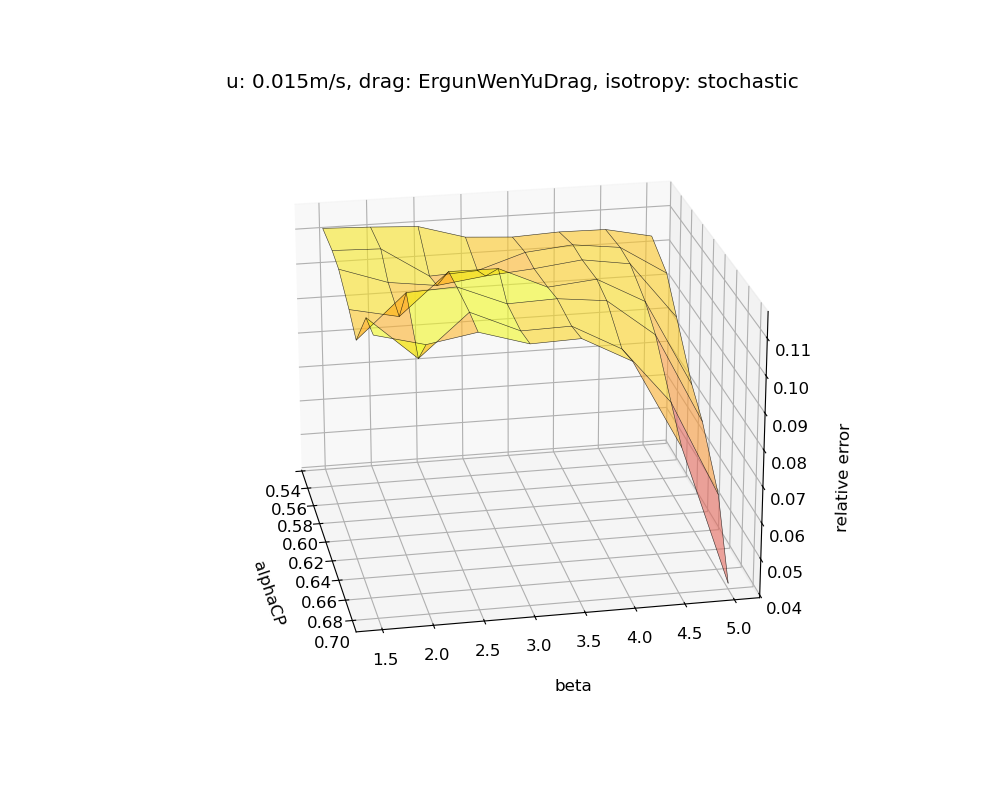
\includegraphics[width = \linewidth, trim = {3.5cm 0 3.5cm 0}, clip]{sections/result/Case 1/Z_heightZ_pres0.015_ErgunWenYuDrag_stochastic.png}
        \caption{Relative error of bed height with drag model \lstinline|ErgunWenYuDrag|, isotropy model \lstinline|stochastic| and inlet velocity $0.015m/s$.}
    \end{subfigure}
\end{figure}

\begin{figure}[h!]
    \centering
    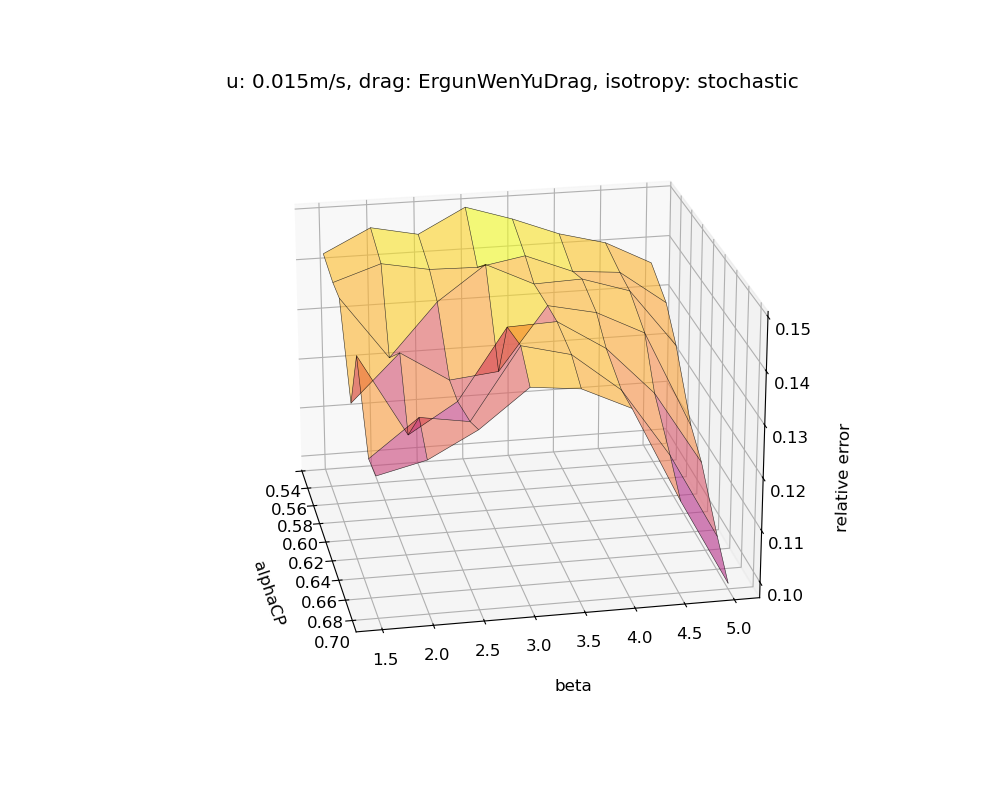
\includegraphics[width=0.5\linewidth, trim = {3.5cm 0 3.5cm 0}, clip]{sections/result/Case 1/Z_bothZ_heightZ_pres0.015_ErgunWenYuDrag_stochastic.png}
    \caption{Combined relative error with drag model \lstinline|ErgunWenYuDrag|, isotropy model \lstinline|stochastic| and inlet velocity $0.015m/s$, according to equation \eqref{eq:relError}.}
    \label{fig:placeholder}
\end{figure}
\FloatBarrier


\paragraph{Drag model \lstinline|PlessisMaliyahDrag| and isotropy model \lstinline|none|}
\FloatBarrier
\begin{figure}[h!]
    \centering
    \begin{subfigure}[b]{0.49 \linewidth}
        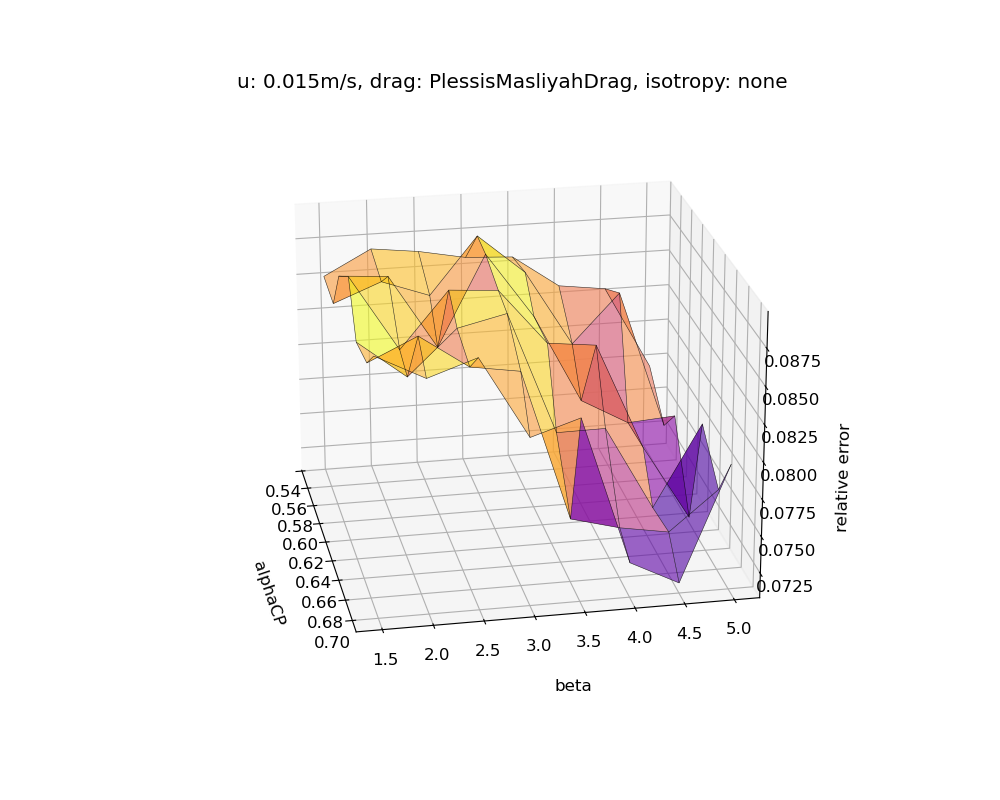
\includegraphics[width = \linewidth, trim = {3.5cm 0 3.5cm 0}, clip]{sections/result/Case 1/Z_pres0.015_PlessisMasliyahDrag_none.png}
        \caption{Relative error of pressure with drag model \lstinline|PlessisMasliyahDrag|, isotropy model \lstinline|none| and inlet velocity $0.015m/s$.}
    \end{subfigure}
    \hfill
    \begin{subfigure}[b]{0.49 \linewidth}
        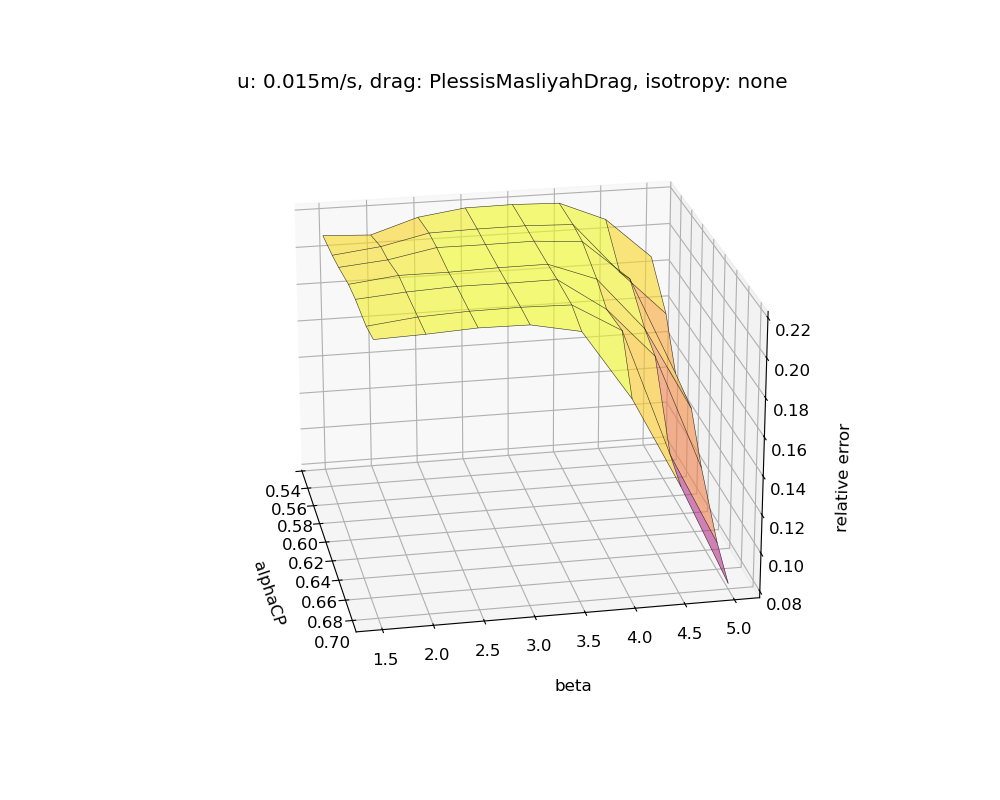
\includegraphics[width = \linewidth, trim = {3.5cm 0 3.5cm 0}, clip]{sections/result/Case 1/Z_heightZ_pres0.015_PlessisMasliyahDrag_none.png}
        \caption{Relative error of bed height with drag model \lstinline|PlessisMasliyahDrag|, isotropy model \lstinline|none| and inlet velocity $0.015m/s$.}
    \end{subfigure}
\end{figure}

\begin{figure}[h!]
    \centering
    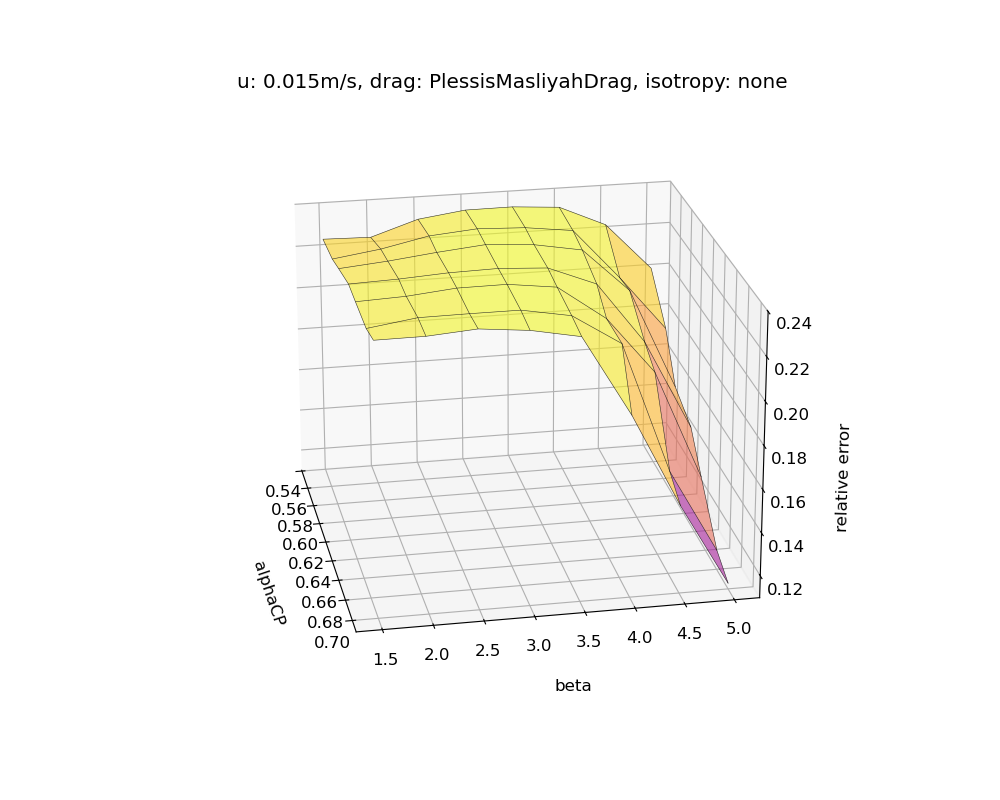
\includegraphics[width=0.5\linewidth, trim = {3.5cm 0 3.5cm 0}, clip]{sections/result/Case 1/Z_bothZ_heightZ_pres0.015_PlessisMasliyahDrag_none.png}
    \caption{Combined relative error with drag model \lstinline|PlessisMasliyahDrag|, isotropy model \lstinline|none| and inlet velocity $0.015m/s$, according to equation \eqref{eq:relError}.}
    \label{fig:placeholder}
\end{figure}
\FloatBarrier



\paragraph{Drag model \lstinline|PlessisMaliyahDrag| and isotropy model \lstinline|stochastic|}

\FloatBarrier
\begin{figure}[h!]
    \centering
    \begin{subfigure}[b]{0.49 \linewidth}
        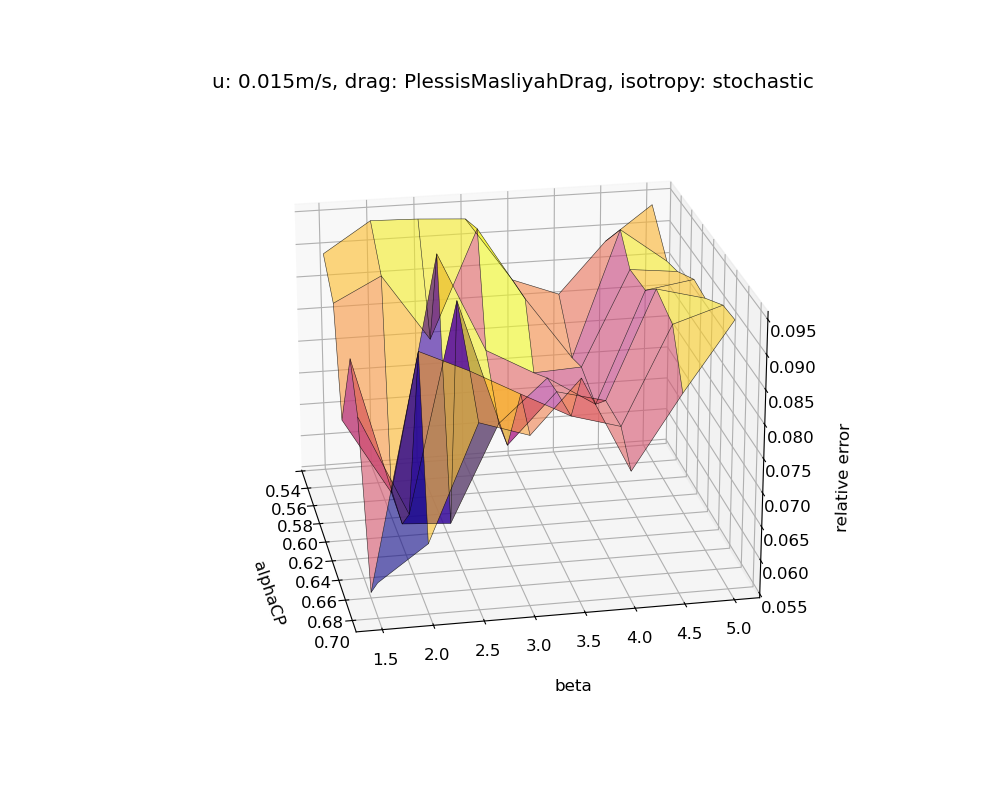
\includegraphics[width = \linewidth, trim = {3.5cm 0 3.5cm 0}, clip]{sections/result/Case 1/Z_pres0.015_PlessisMasliyahDrag_stochastic.png}
        \caption{Relative error of pressure with drag model \lstinline|PlessisMasliyahDrag|, isotropy model \lstinline|none| and inlet velocity $0.015m/s$.}
    \end{subfigure}
    \begin{subfigure}[b]{0.49 \linewidth}
        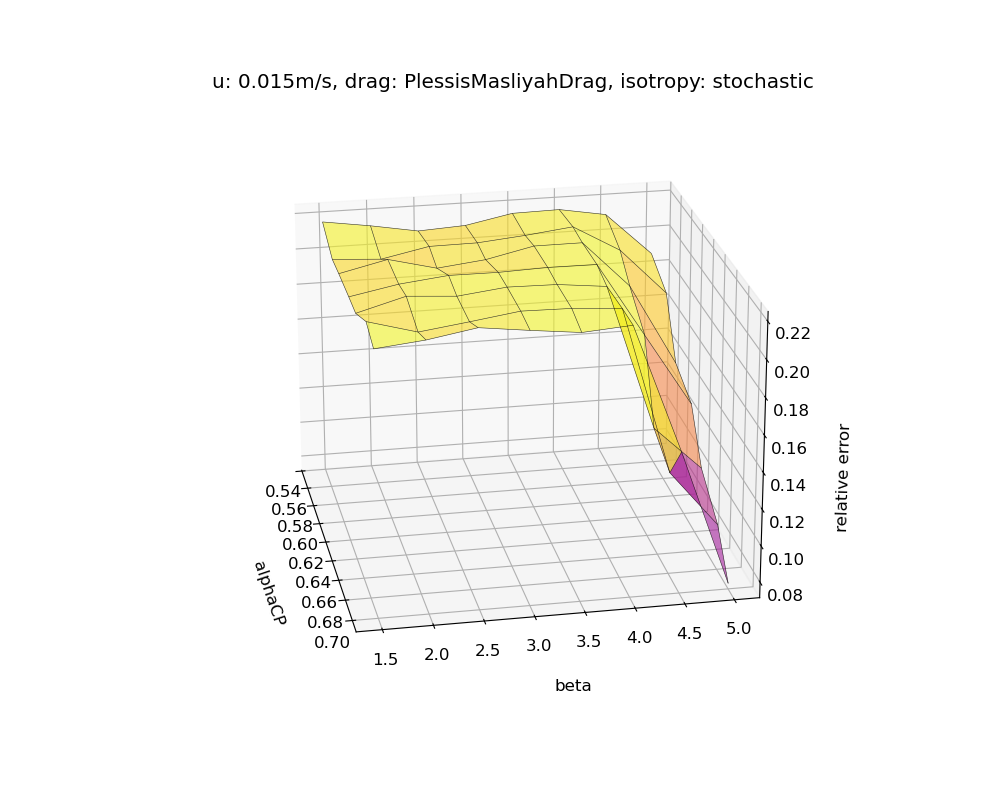
\includegraphics[width = \linewidth, trim = {3.5cm 0 3.5cm 0}, clip]{sections/result/Case 1/Z_heightZ_pres0.015_PlessisMasliyahDrag_stochastic.png}
        \caption{Relative error of bed height with drag model \lstinline|PlessisMasliyahDrag|, isotropy model \lstinline|stochastic| and inlet velocity $0.015m/s$.}
    \end{subfigure}
\end{figure}

\begin{figure}[h!]
    \centering
    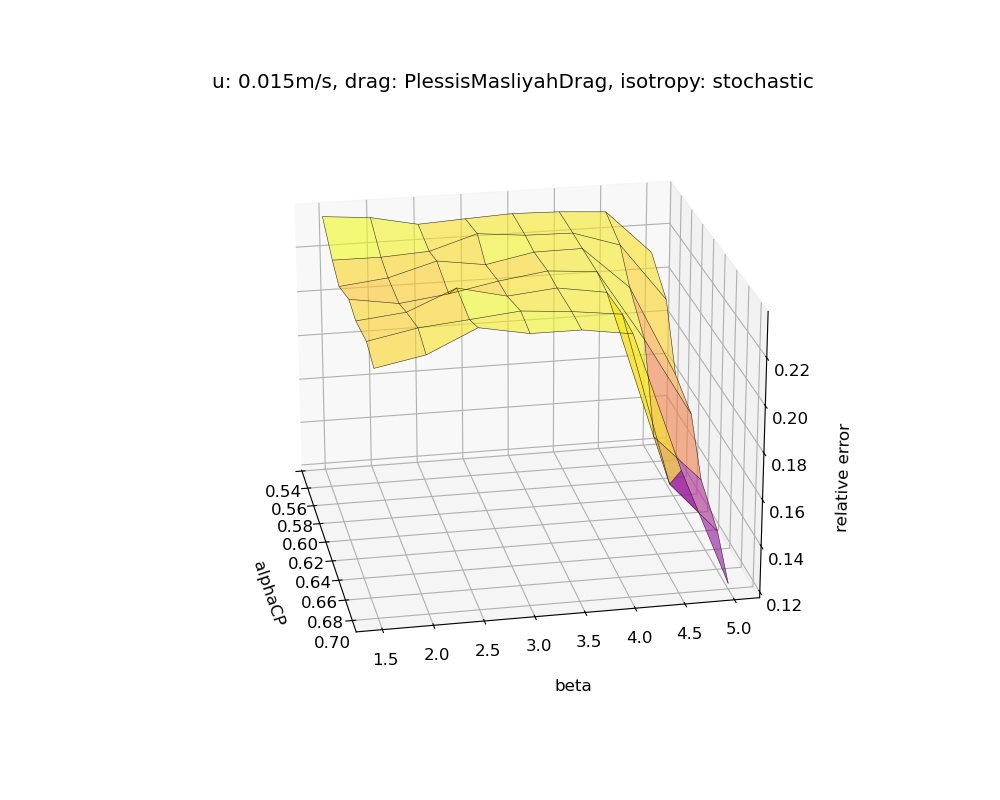
\includegraphics[width=0.5\linewidth, trim = {3.5cm 0 3.5cm 0}, clip]{sections/result/Case 1/Z_bothZ_heightZ_pres0.015_PlessisMasliyahDrag_stochastic.png}
    \caption{Combined relative error with drag model \lstinline|PlessisMasliyahDrag|, isotropy model \lstinline|stochastic| and inlet velocity $0.015m/s$, according to equation \eqref{eq:relError}.}
    \label{fig:placeholder}
\end{figure}
\FloatBarrier


\subsubsection{Inlet velocity $\uf = 0.025 m/s$}
\paragraph{Drag model \lstinline|ErgunWenYuDrag| and isotropy model \lstinline|none|}
\FloatBarrier
\begin{figure}[h!]
    \centering
    \begin{subfigure}[b]{0.49 \linewidth}
        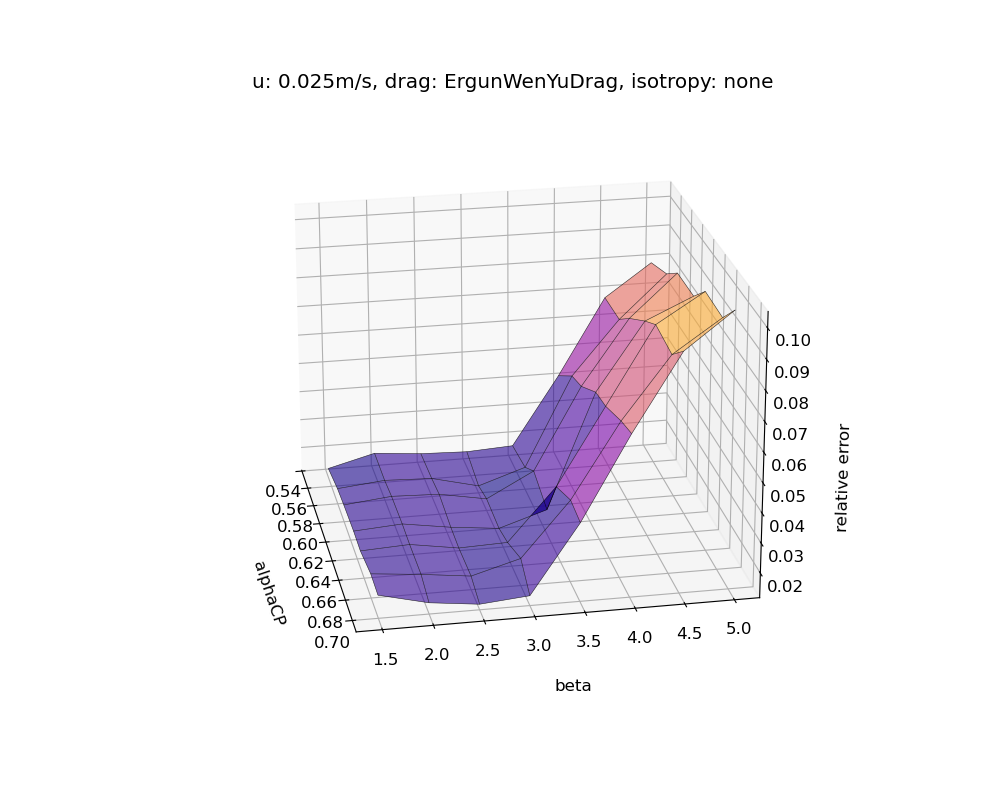
\includegraphics[width = \linewidth, trim = {3.5cm 0 3.5cm 0}, clip]{sections/result/Case 1/Z_pres0.025_ErgunWenYuDrag_none.png}
        \caption{Relative error of pressure with drag model \lstinline|ErgunWenYuDrag|, isotropy model \lstinline|none| and inlet velocity $0.025m/s$.}
    \end{subfigure}
    \hfill
    \begin{subfigure}[b]{0.49 \linewidth}
        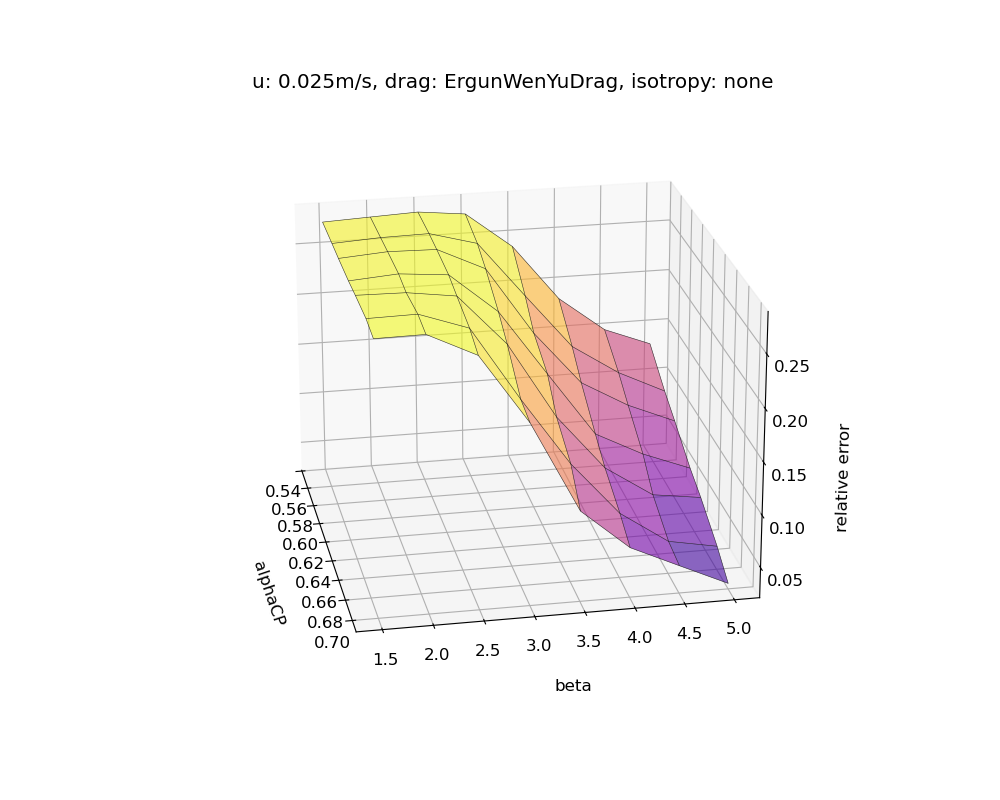
\includegraphics[width = \linewidth, trim = {3.5cm 0 3.5cm 0}, clip]{sections/result/Case 1/Z_height0.025_ErgunWenYuDrag_none.png}
        \caption{Relative error of bed height with drag model \lstinline|ErgunWenYuDrag|, isotropy model \lstinline|none| and inlet velocity $0.025m/s$.}
    \end{subfigure}
\end{figure}

\begin{figure}[h!]
    \centering
    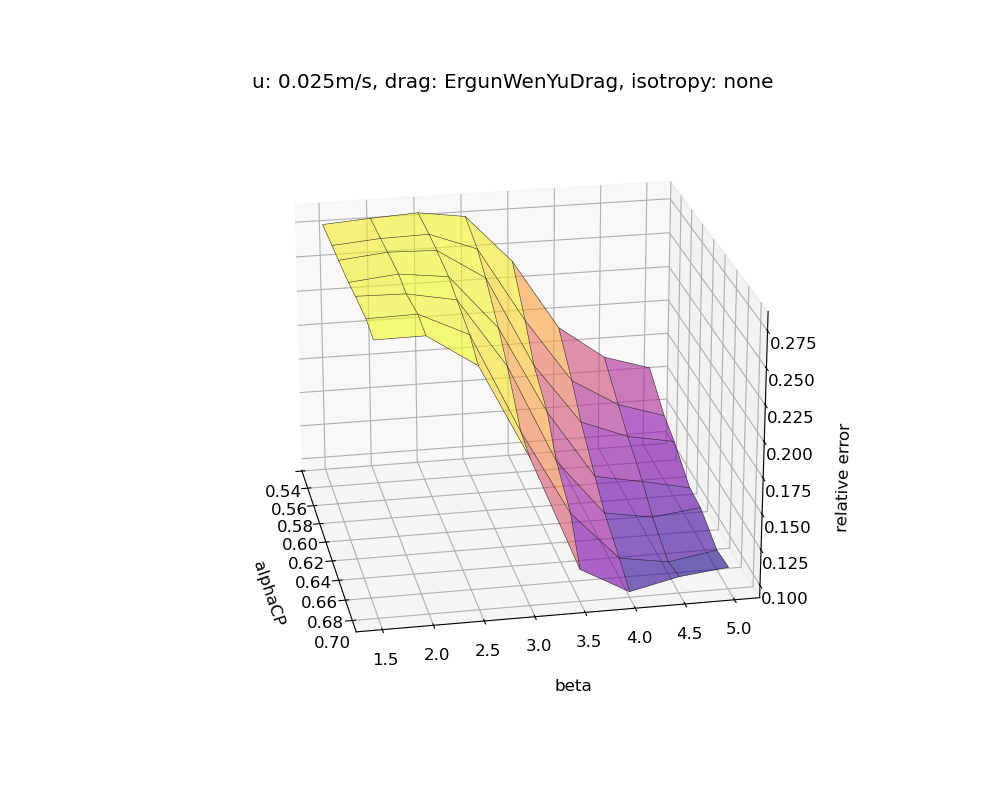
\includegraphics[width=0.5\linewidth, trim = {3.5cm 0 3.5cm 0}, clip]{sections/result/Case 1/Z_both0.025_ErgunWenYuDrag_none.png}
    \caption{Combined relative error with drag model \lstinline|ErgunWenYuDrag|, isotropy model \lstinline|none| and inlet velocity $0.025m/s$, according to equation \eqref{eq:relError}.}
    \label{fig:placeholder}
\end{figure}
\FloatBarrier


\paragraph{Drag model \lstinline|ErgunWenYu| and isotropy model \lstinline|stochastic|}
\FloatBarrier
\begin{figure}[h!]
    \centering
    \begin{subfigure}[b]{0.49 \linewidth}
        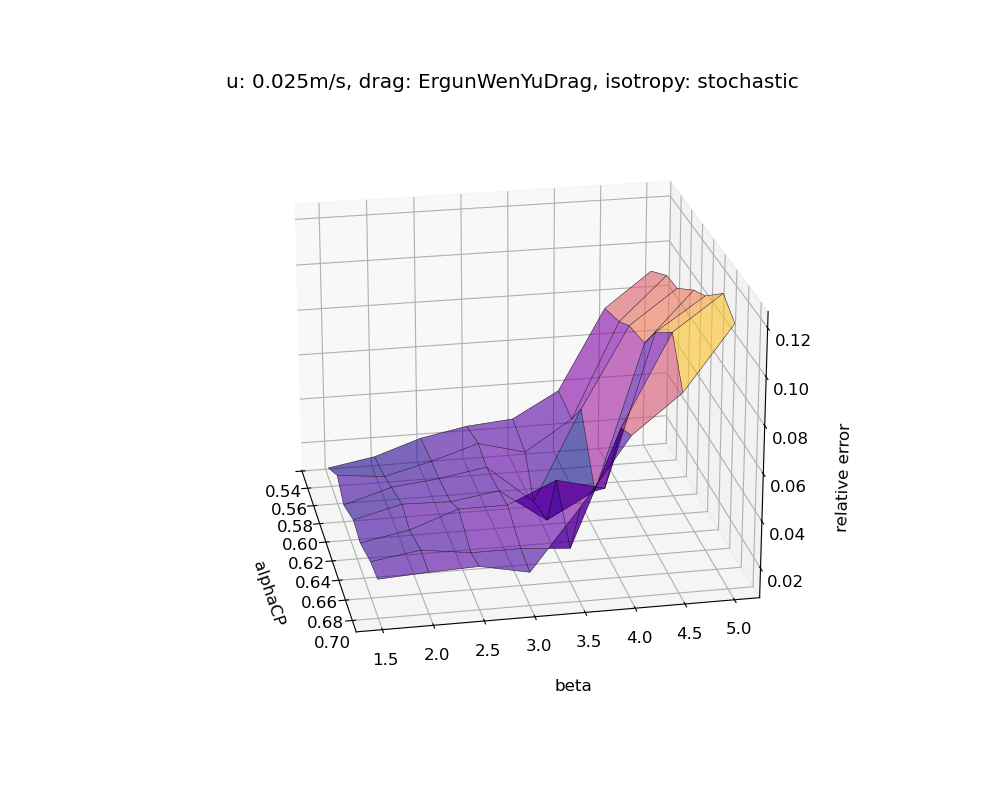
\includegraphics[width = \linewidth, trim = {3.5cm 0 3.5cm 0}, clip]{sections/result/Case 1/Z_pres0.025_ErgunWenYuDrag_stochastic.png}
        \caption{Relative error of pressure with drag model \lstinline|ErgunWenYuDrag|, isotropy model \lstinline|stochastic| and inlet velocity $0.025m/s$.}
    \end{subfigure}
    \hfill
    \begin{subfigure}[b]{0.49 \linewidth}
        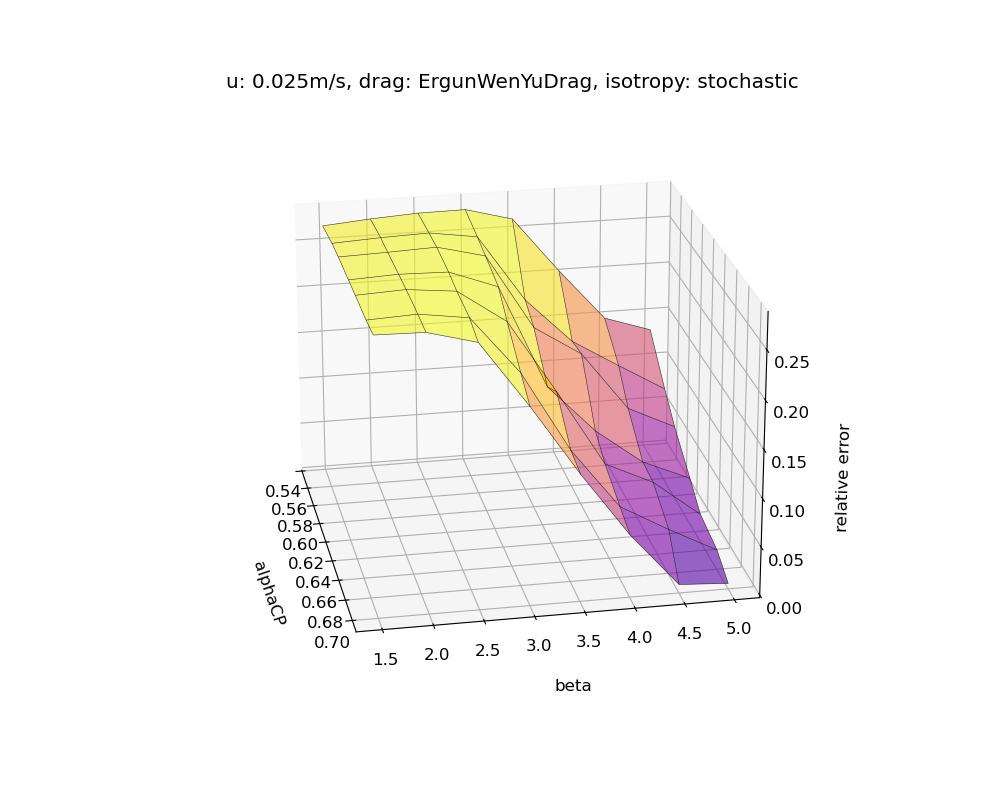
\includegraphics[width = \linewidth, trim = {3.5cm 0 3.5cm 0}, clip]{sections/result/Case 1/Z_height0.025_ErgunWenYuDrag_stochastic.png}
        \caption{Relative error of bed height with drag model \lstinline|ErgunWenYuDrag|, isotropy model \lstinline|stochastic| and inlet velocity $0.025m/s$.}
    \end{subfigure}
\end{figure}

\begin{figure}[h!]
    \centering
    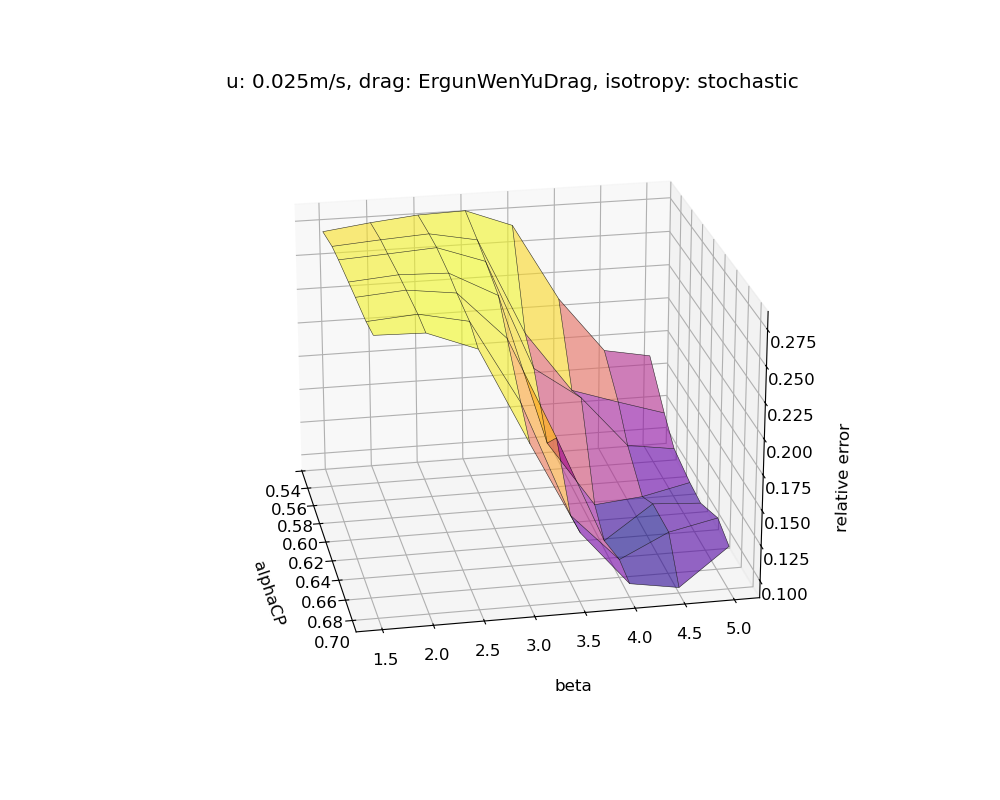
\includegraphics[width=0.5\linewidth, trim = {3.5cm 0 3.5cm 0}, clip]{sections/result/Case 1/Z_both0.025_ErgunWenYuDrag_stochastic.png}
    \caption{Combined relative error with drag model \lstinline|ErgunWenYuDrag|, isotropy model \lstinline|stochastic| and inlet velocity $0.025m/s$, according to equation \eqref{eq:relError}.}
    \label{fig:placeholder}
\end{figure}
\FloatBarrier


\paragraph{Drag model \lstinline|PlessisMaliyahDrag| and isotropy model \lstinline|none|}
\FloatBarrier
\begin{figure}[h!]
    \centering
    \begin{subfigure}[b]{0.49 \linewidth}
        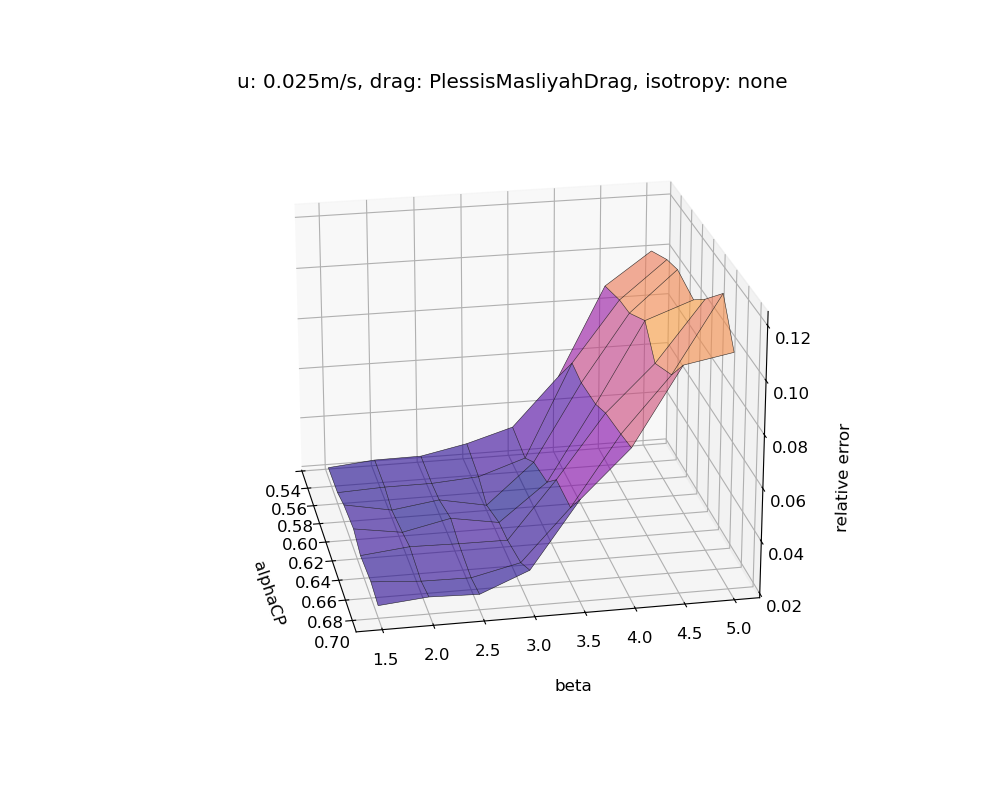
\includegraphics[width = \linewidth, trim = {3.5cm 0 3.5cm 0}, clip]{sections/result/Case 1/Z_pres0.025_PlessisMasliyahDrag_none.png}
        \caption{Relative error of pressure with drag model \lstinline|PlessisMasliyahDrag|, isotropy model \lstinline|none| and inlet velocity $0.025m/s$.}
    \end{subfigure}
    \hfill
    \begin{subfigure}[b]{0.49 \linewidth}
        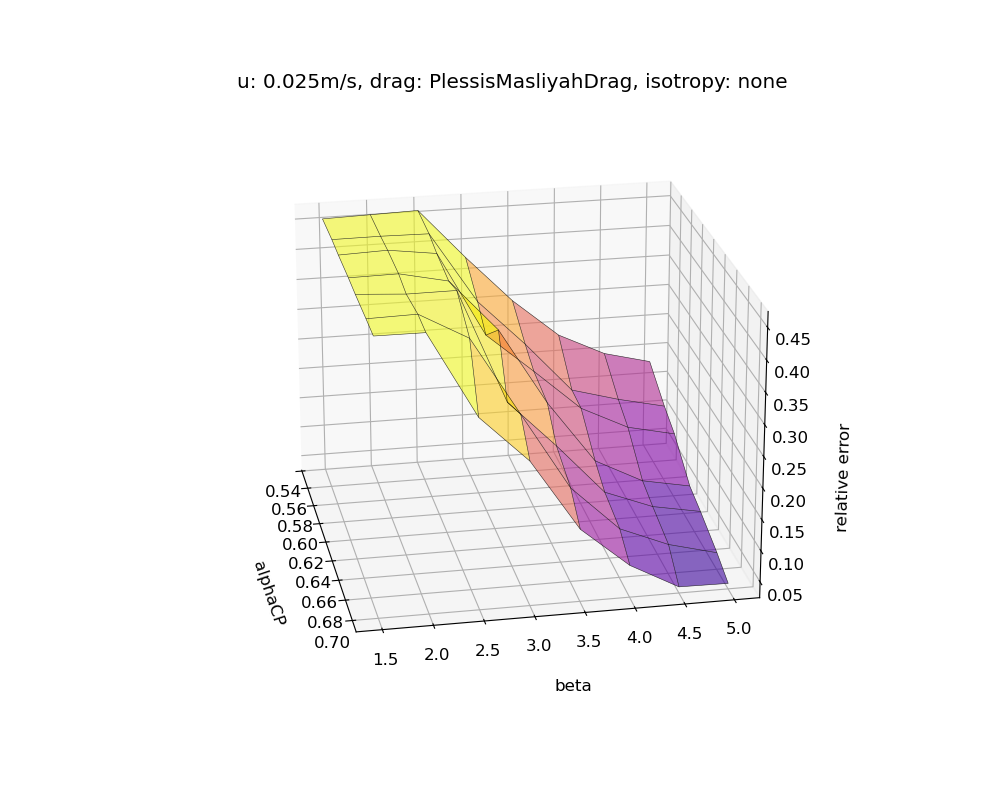
\includegraphics[width = \linewidth, trim = {3.5cm 0 3.5cm 0}, clip]{sections/result/Case 1/Z_height0.025_PlessisMasliyahDrag_none.png}
        \caption{Relative error of bed height with drag model \lstinline|PlessisMasliyahDrag|, isotropy model \lstinline|none| and inlet velocity $0.025m/s$.}
    \end{subfigure}
\end{figure}

\begin{figure}[h!]
    \centering
    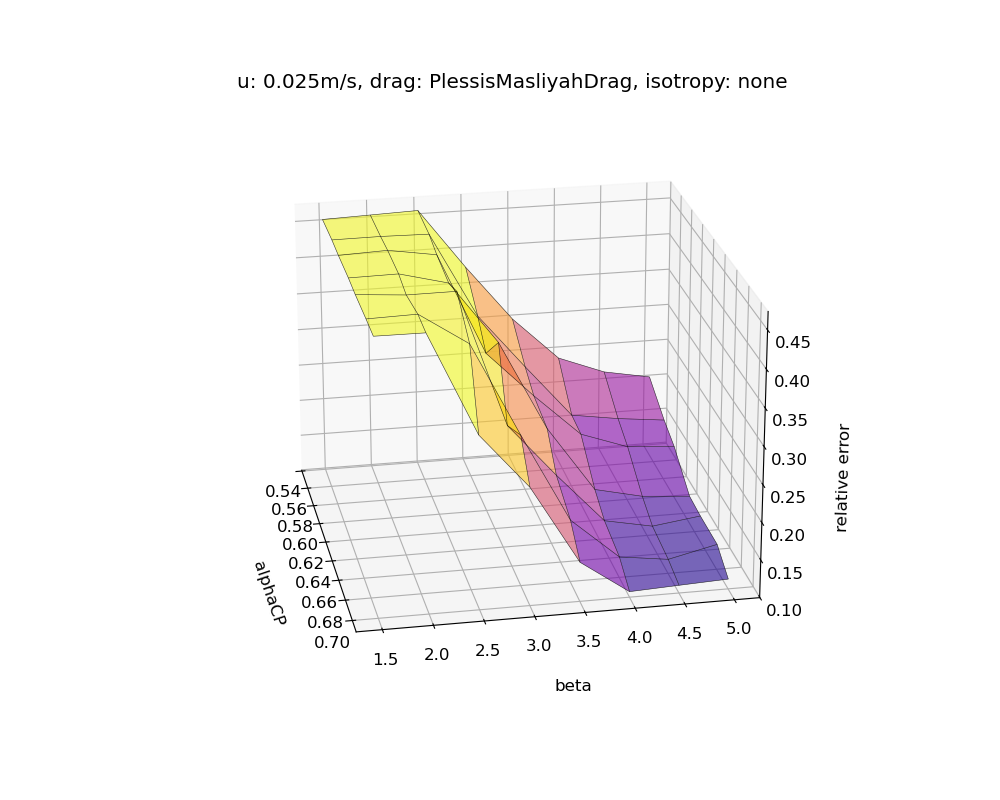
\includegraphics[width=0.5\linewidth, trim = {3.5cm 0 3.5cm 0}, clip]{sections/result/Case 1/Z_both0.025_PlessisMasliyahDrag_none.png}
    \caption{Combined relative error with drag model \lstinline|PlessisMasliyahDrag|, isotropy model \lstinline|none| and inlet velocity $0.025m/s$, according to equation \eqref{eq:relError}.}
    \label{fig:placeholder}
\end{figure}
\FloatBarrier



\paragraph{Drag model \lstinline|PlessisMaliyahDrag| and isotropy model \lstinline|stochastic|}

\FloatBarrier
\begin{figure}[h!]
    \centering
    \begin{subfigure}[b]{0.49 \linewidth}
        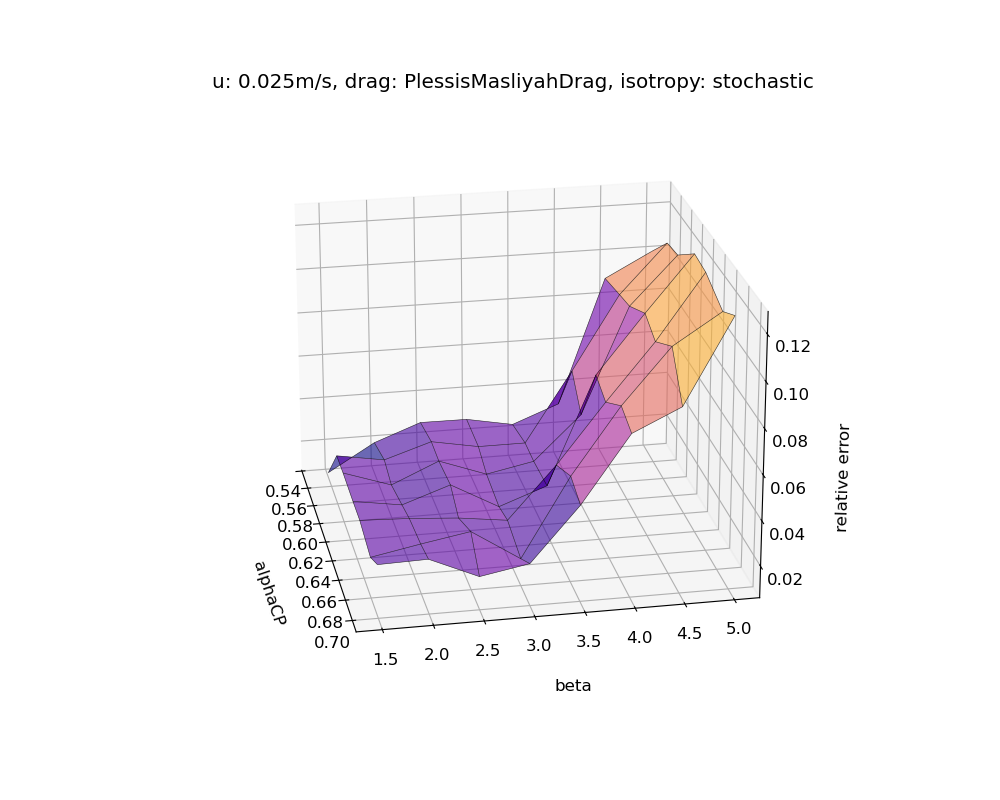
\includegraphics[width = \linewidth, trim = {3.5cm 0 3.5cm 0}, clip]{sections/result/Case 1/Z_pres0.025_PlessisMasliyahDrag_stochastic.png}
        \caption{Relative error of pressure with drag model \lstinline|PlessisMasliyahDrag|, isotropy model \lstinline|none| and inlet velocity $0.025m/s$.}
    \end{subfigure}
    \begin{subfigure}[b]{0.49 \linewidth}
        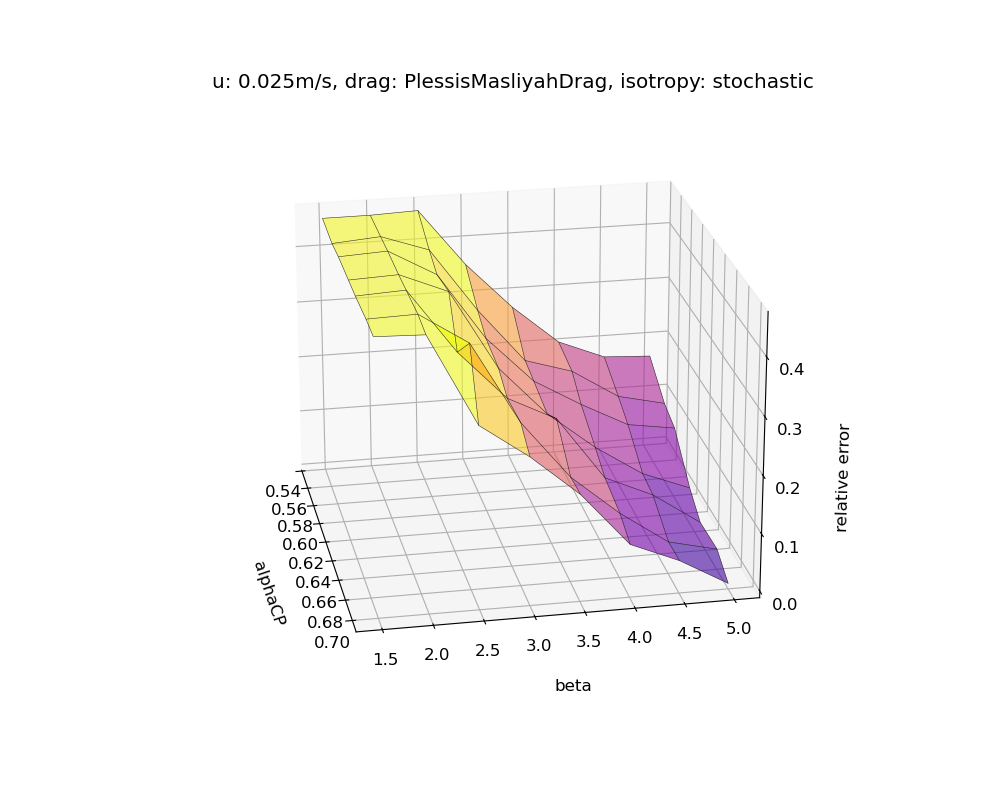
\includegraphics[width = \linewidth, trim = {3.5cm 0 3.5cm 0}, clip]{sections/result/Case 1/Z_height0.025_PlessisMasliyahDrag_stochastic.png}
        \caption{Relative error of bed height with drag model \lstinline|PlessisMasliyahDrag|, isotropy model \lstinline|stochastic| and inlet velocity $0.025m/s$.}
    \end{subfigure}
\end{figure}

\begin{figure}[h!]
    \centering
    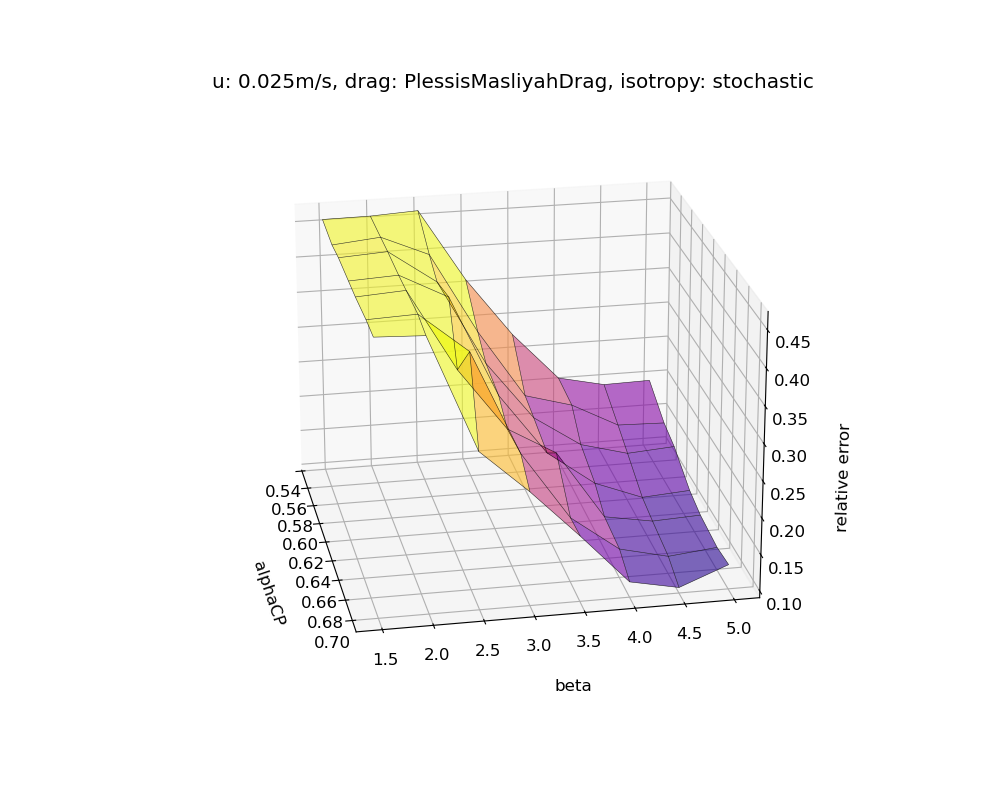
\includegraphics[width=0.5\linewidth, trim = {3.5cm 0 3.5cm 0}, clip]{sections/result/Case 1/Z_both0.025_PlessisMasliyahDrag_stochastic.png}
    \caption{Combined relative error with drag model \lstinline|PlessisMasliyahDrag|, isotropy model \lstinline|stochastic| and inlet velocity $0.025m/s$, according to equation \eqref{eq:relError}.}
    \label{fig:placeholder}
\end{figure}
\FloatBarrier



\subsection{Case 2: $\pvfcp$ and $P_s$}
In this section we look at the second case where the close pack volume fraction $\pvfcp$ and the pressure constant $P_s$ are varied. The exponent $\beta$ is left constant.
We test the parameters for four inlet velocities.

\subsubsection{Inlet velocity $\uf = 0.015 m/s$}
\paragraph{Drag model \lstinline|ErgunWenYuDrag| and isotropy model \lstinline|none|}
% \FloatBarrier
% \begin{figure}[h!]
%     \centering
%     \begin{subfigure}[b]{0.49 \linewidth}
%         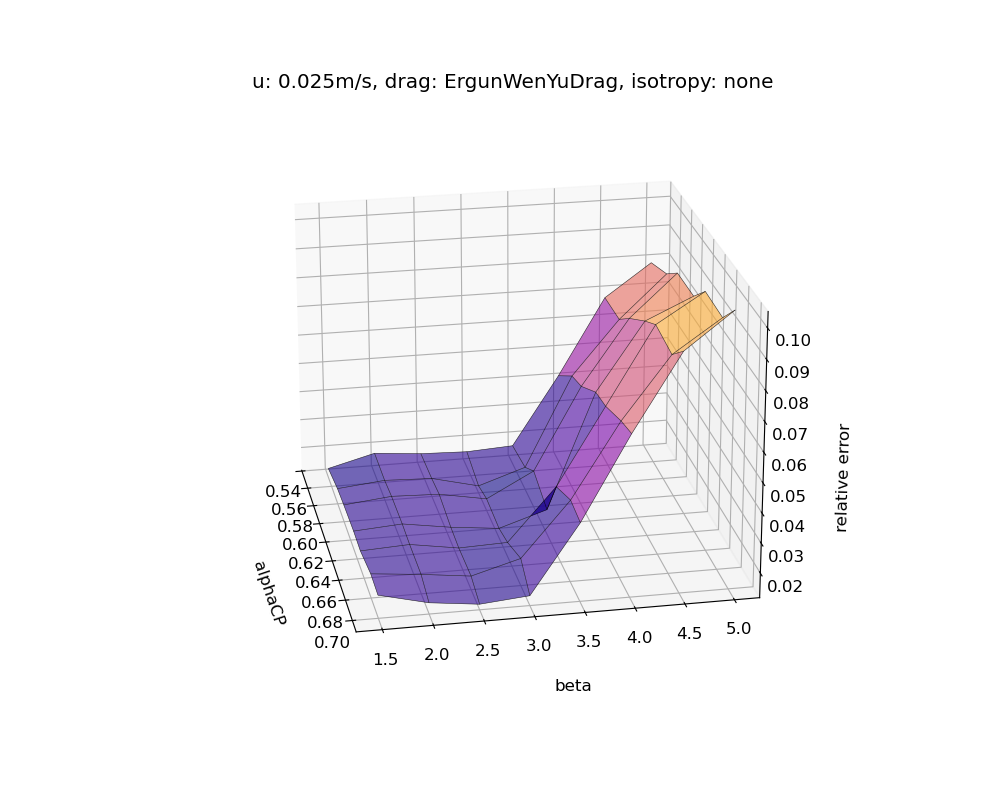
\includegraphics[width = \linewidth, trim = {3.5cm 0 3.5cm 0}, clip]{sections/result/Case 1/Z_pres0.025_ErgunWenYuDrag_none.png}
%         \caption{Relative error of pressure with drag model \lstinline|ErgunWenYuDrag|, isotropy model \lstinline|none| and inlet velocity $0.025m/s$.}
%     \end{subfigure}
%     \hfill
%     \begin{subfigure}[b]{0.49 \linewidth}
%         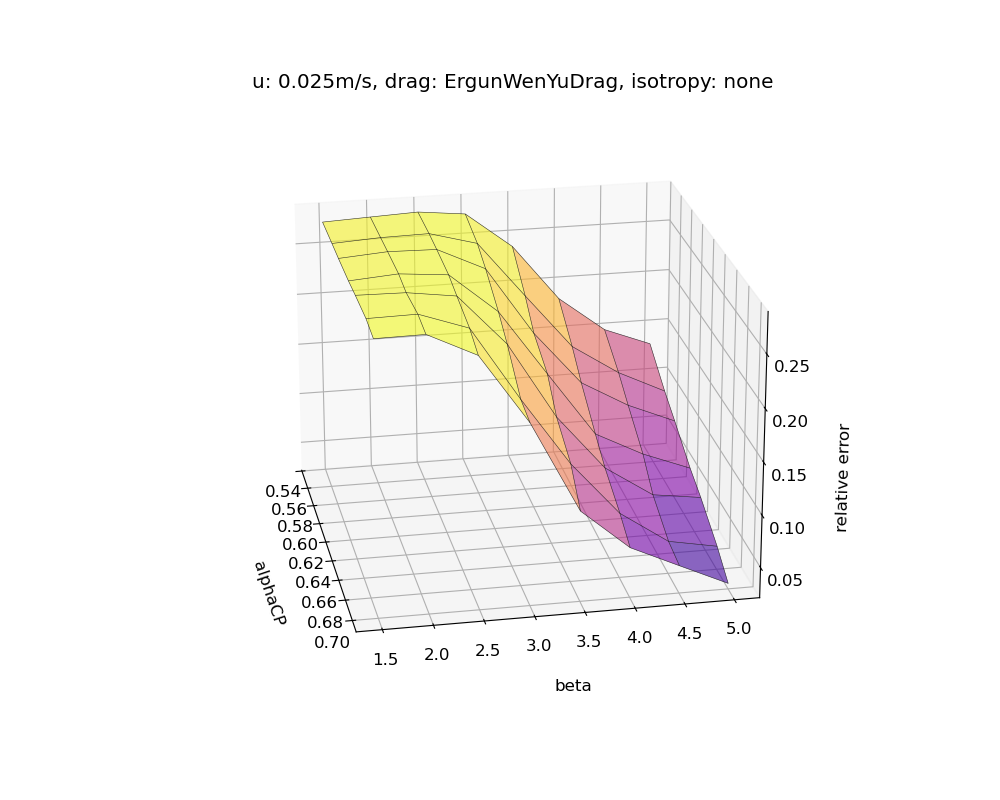
\includegraphics[width = \linewidth, trim = {3.5cm 0 3.5cm 0}, clip]{sections/result/Case 1/Z_height0.025_ErgunWenYuDrag_none.png}
%         \caption{Relative error of bed height with drag model \lstinline|ErgunWenYuDrag|, isotropy model \lstinline|none| and inlet velocity $0.025m/s$.}
%     \end{subfigure}
% \end{figure}

% \begin{figure}[h!]
%     \centering
%     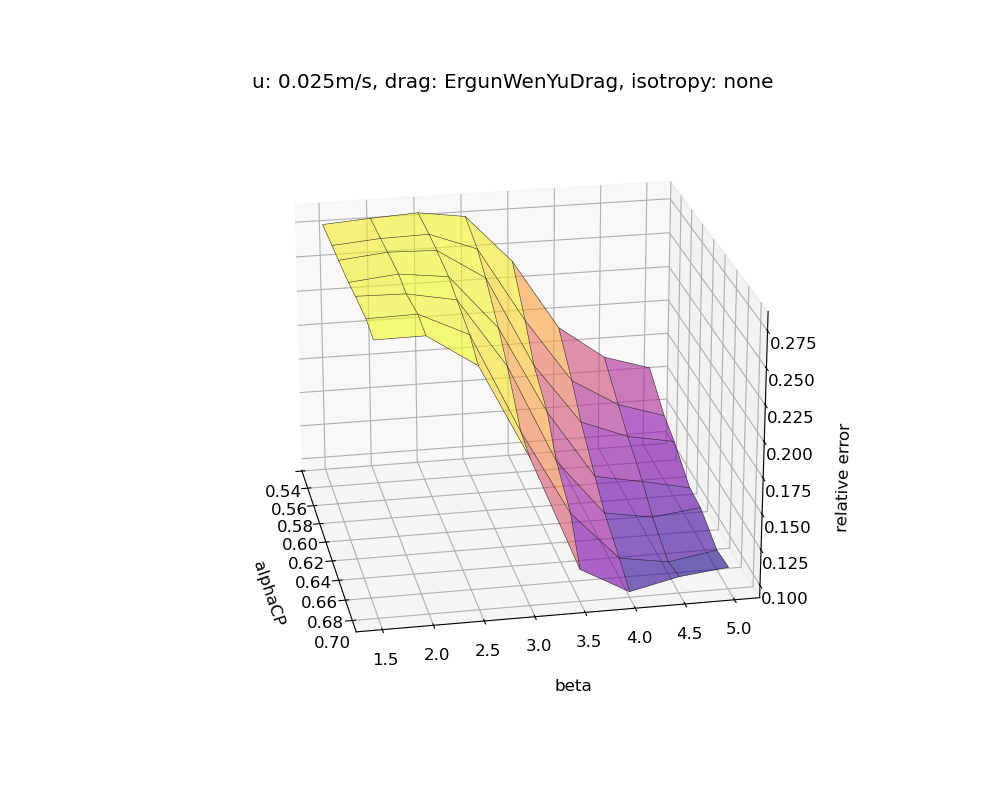
\includegraphics[width=0.5\linewidth, trim = {3.5cm 0 3.5cm 0}, clip]{sections/result/Case 1/Z_both0.025_ErgunWenYuDrag_none.png}
%     \caption{Combined relative error with drag model \lstinline|ErgunWenYuDrag|, isotropy model \lstinline|none| and inlet velocity $0.025m/s$, according to equation \eqref{eq:relError}.}
%     \label{fig:placeholder}
% \end{figure}
% \FloatBarrier


\paragraph{Drag model \lstinline|ErgunWenYu| and isotropy model \lstinline|stochastic|}
\FloatBarrier
\begin{figure}[h!]
    \centering
    \begin{subfigure}[b]{0.49 \linewidth}
        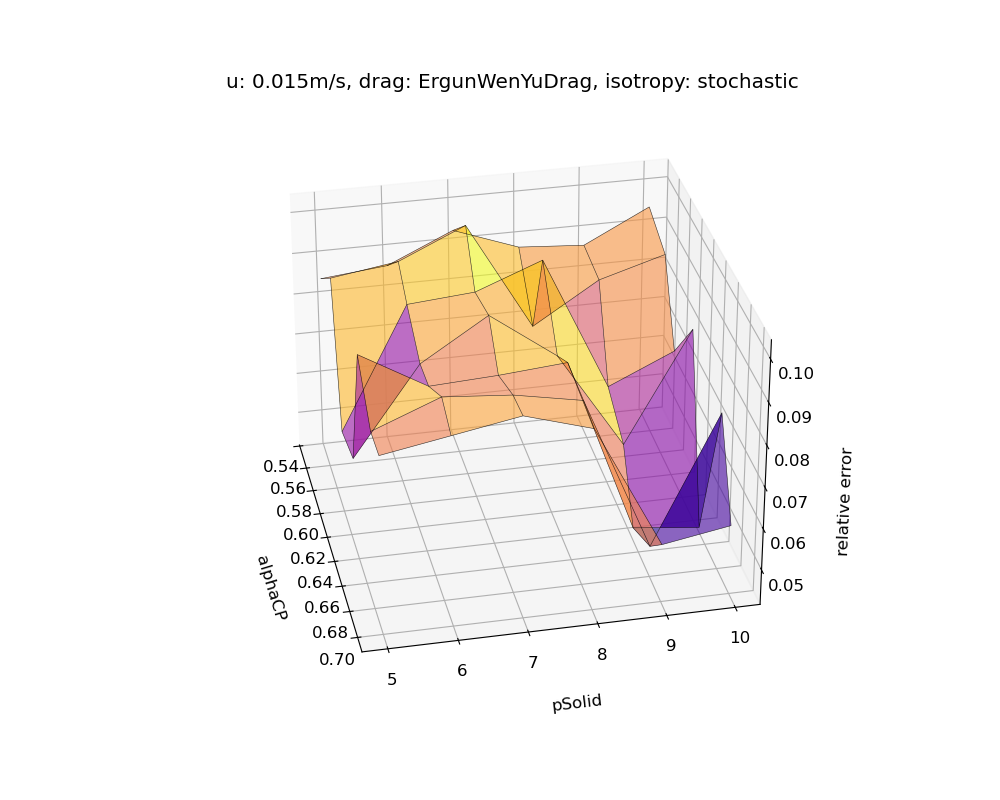
\includegraphics[width = \linewidth, trim = {3.5cm 0 3.5cm 0}, clip]{sections/result/Case 2/Z_pres0.015_ErgunWenYuDrag_stochastic.png}
        \caption{Relative error of pressure with drag model \lstinline|ErgunWenYuDrag|, isotropy model \lstinline|stochastic| and inlet velocity $0.015m/s$.}
    \end{subfigure}
    \hfill
    \begin{subfigure}[b]{0.49 \linewidth}
        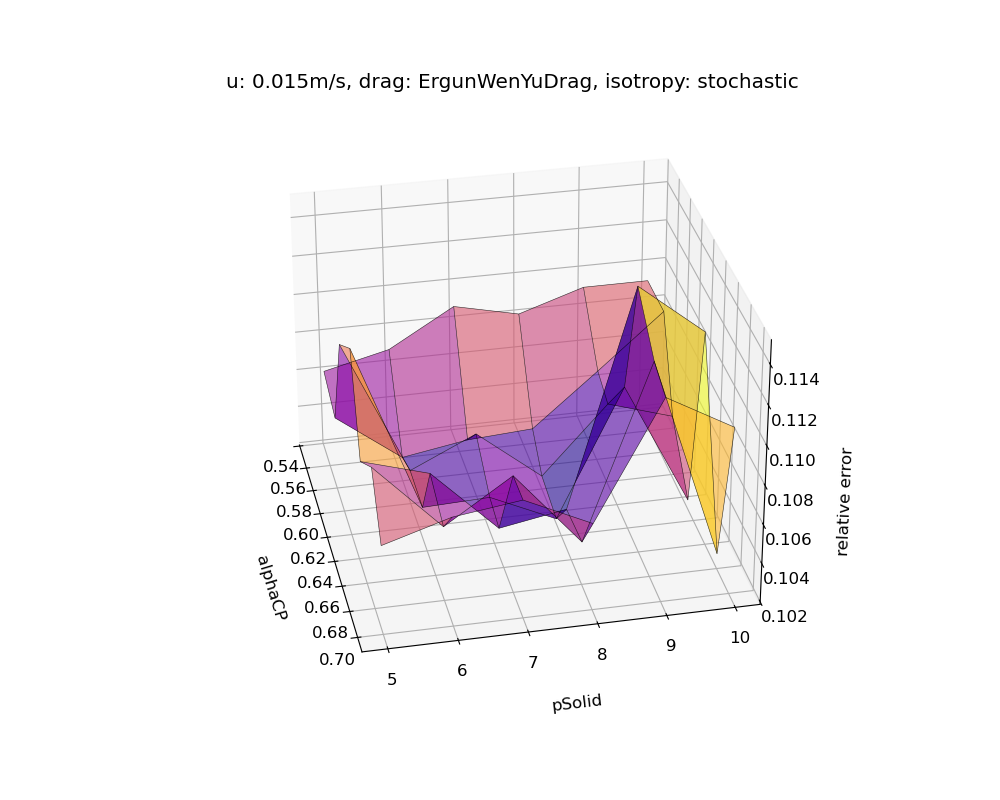
\includegraphics[width = \linewidth, trim = {3.5cm 0 3.5cm 0}, clip]{sections/result/Case 2/Z_height0.015_ErgunWenYuDrag_stochastic.png}
        \caption{Relative error of bed height with drag model \lstinline|ErgunWenYuDrag|, isotropy model \lstinline|stochastic| and inlet velocity $0.015m/s$.}
    \end{subfigure}
\end{figure}

\begin{figure}[h!]
    \centering
    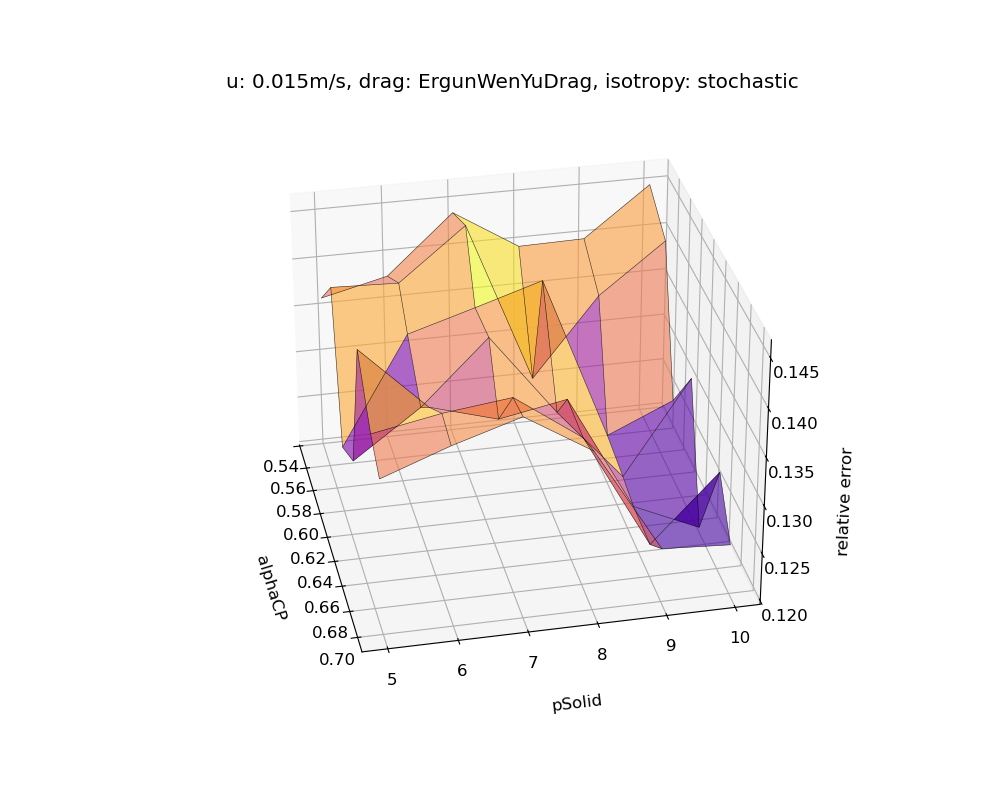
\includegraphics[width=0.5\linewidth, trim = {3.5cm 0 3.5cm 0}, clip]{sections/result/Case 2/Z_both0.015_ErgunWenYuDrag_stochastic.png}
    \caption{Combined relative error with drag model \lstinline|ErgunWenYuDrag|, isotropy model \lstinline|stochastic| and inlet velocity $0.015m/s$, according to equation \eqref{eq:relError}.}
    \label{fig:placeholder}
\end{figure}
\FloatBarrier


\paragraph{Drag model \lstinline|PlessisMaliyahDrag| and isotropy model \lstinline|none|}
% \FloatBarrier
% \begin{figure}[h!]
%     \centering
%     \begin{subfigure}[b]{0.49 \linewidth}
%         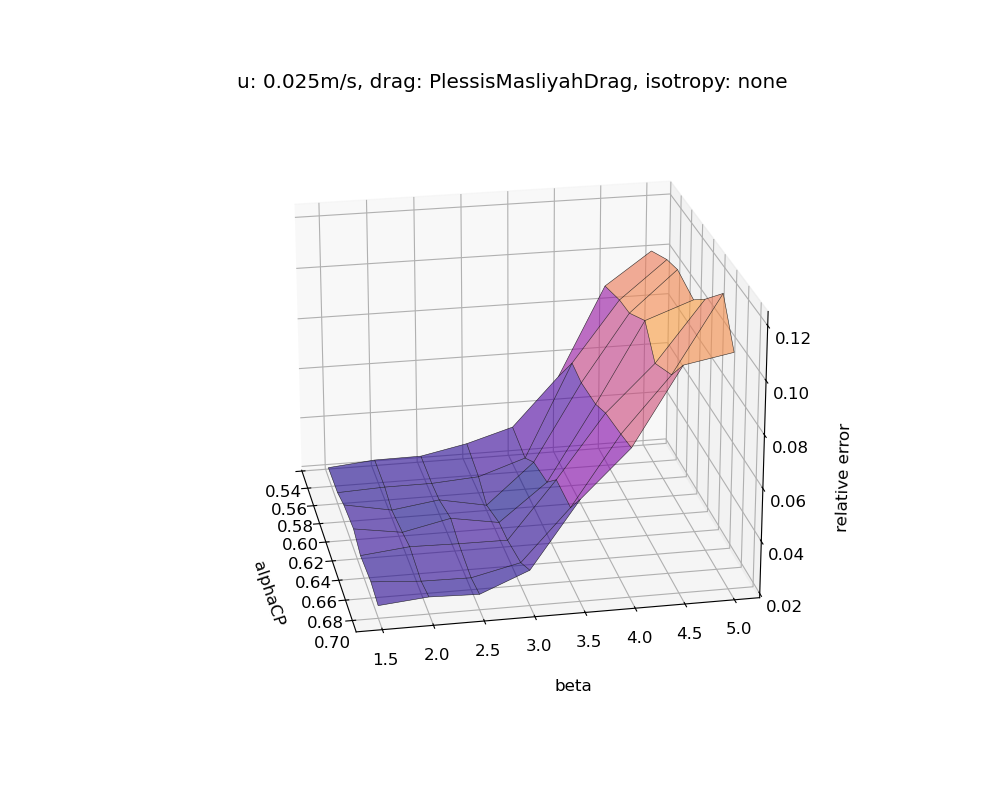
\includegraphics[width = \linewidth, trim = {3.5cm 0 3.5cm 0}, clip]{sections/result/Case 1/Z_pres0.025_PlessisMasliyahDrag_none.png}
%         \caption{Relative error of pressure with drag model \lstinline|PlessisMasliyahDrag|, isotropy model \lstinline|none| and inlet velocity $0.025m/s$.}
%     \end{subfigure}
%     \hfill
%     \begin{subfigure}[b]{0.49 \linewidth}
%         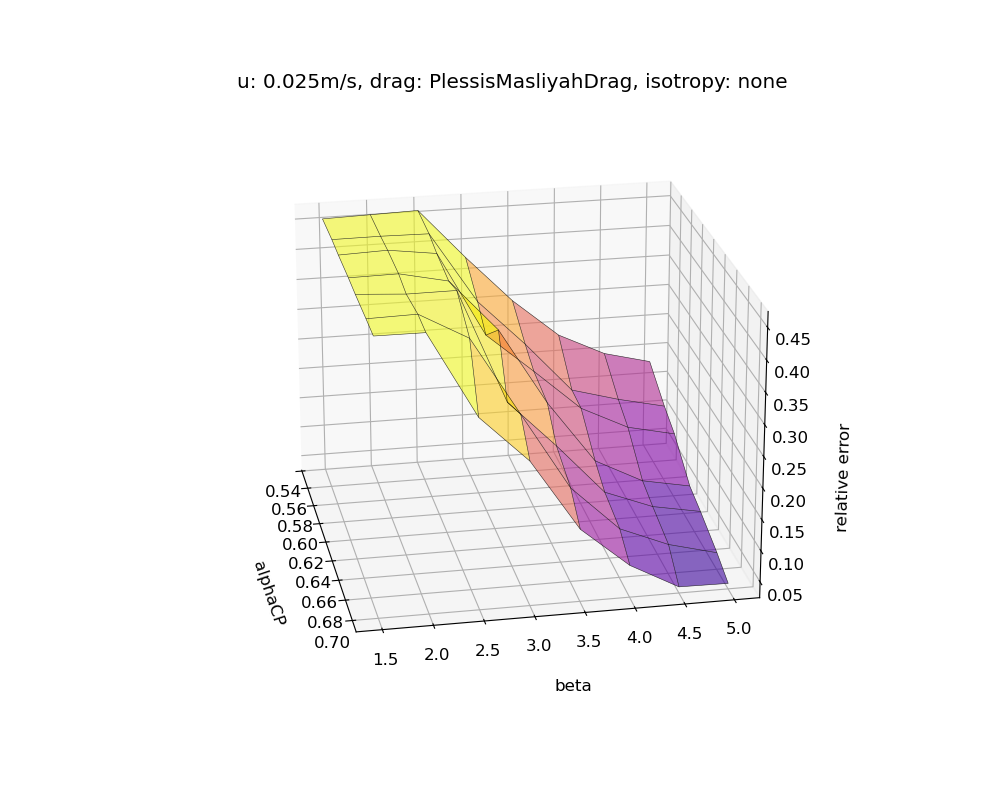
\includegraphics[width = \linewidth, trim = {3.5cm 0 3.5cm 0}, clip]{sections/result/Case 1/Z_height0.025_PlessisMasliyahDrag_none.png}
%         \caption{Relative error of bed height with drag model \lstinline|PlessisMasliyahDrag|, isotropy model \lstinline|none| and inlet velocity $0.025m/s$.}
%     \end{subfigure}
% \end{figure}

% \begin{figure}[h!]
%     \centering
%     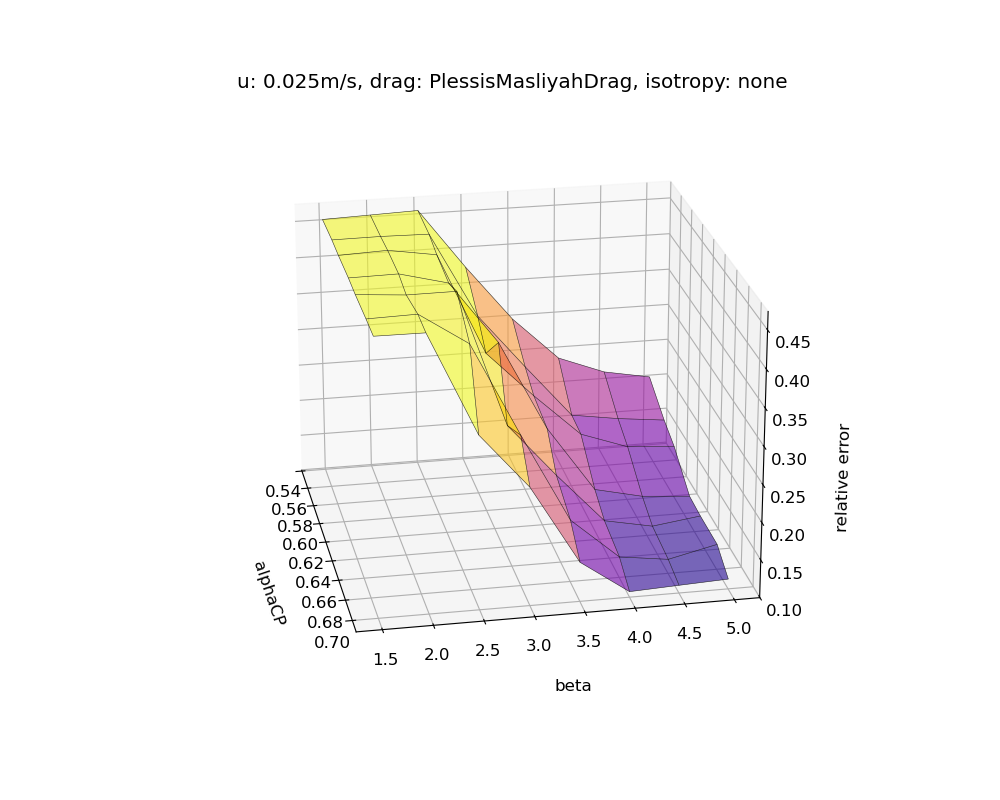
\includegraphics[width=0.5\linewidth, trim = {3.5cm 0 3.5cm 0}, clip]{sections/result/Case 1/Z_both0.025_PlessisMasliyahDrag_none.png}
%     \caption{Combined relative error with drag model \lstinline|PlessisMasliyahDrag|, isotropy model \lstinline|none| and inlet velocity $0.025m/s$, according to equation \eqref{eq:relError}.}
%     \label{fig:placeholder}
% \end{figure}
% \FloatBarrier



\paragraph{Drag model \lstinline|PlessisMaliyahDrag| and isotropy model \lstinline|stochastic|}

% \FloatBarrier
% \begin{figure}[h!]
%     \centering
%     \begin{subfigure}[b]{0.49 \linewidth}
%         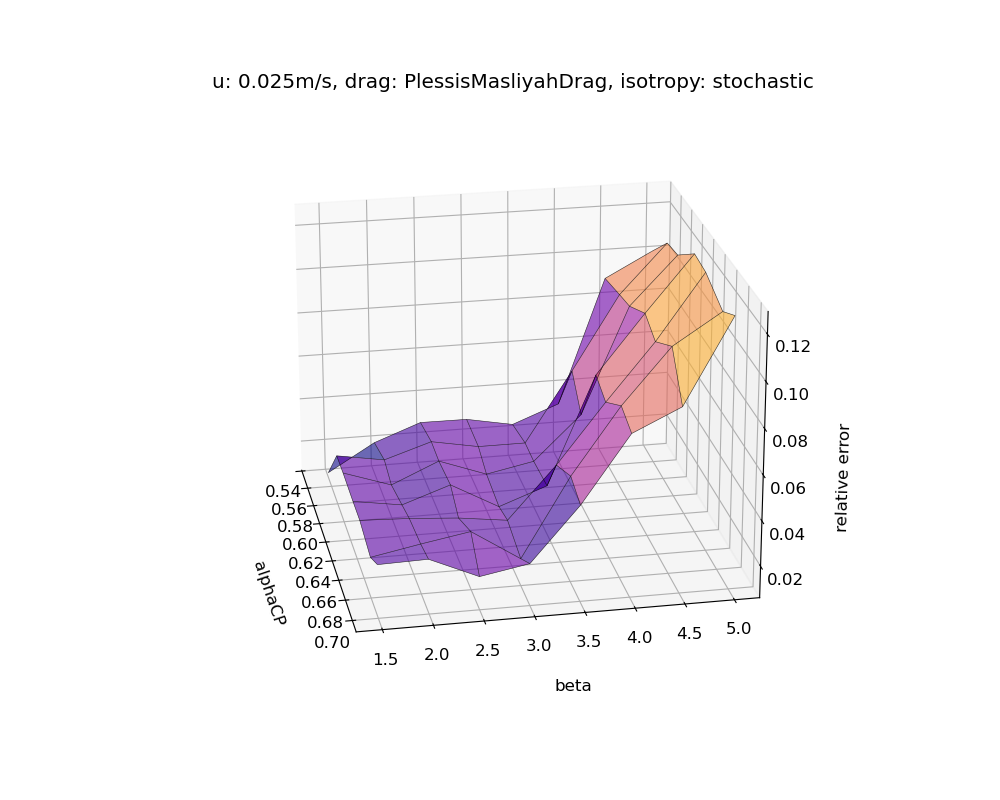
\includegraphics[width = \linewidth, trim = {3.5cm 0 3.5cm 0}, clip]{sections/result/Case 1/Z_pres0.025_PlessisMasliyahDrag_stochastic.png}
%         \caption{Relative error of pressure with drag model \lstinline|PlessisMasliyahDrag|, isotropy model \lstinline|none| and inlet velocity $0.025m/s$.}
%     \end{subfigure}
%     \begin{subfigure}[b]{0.49 \linewidth}
%         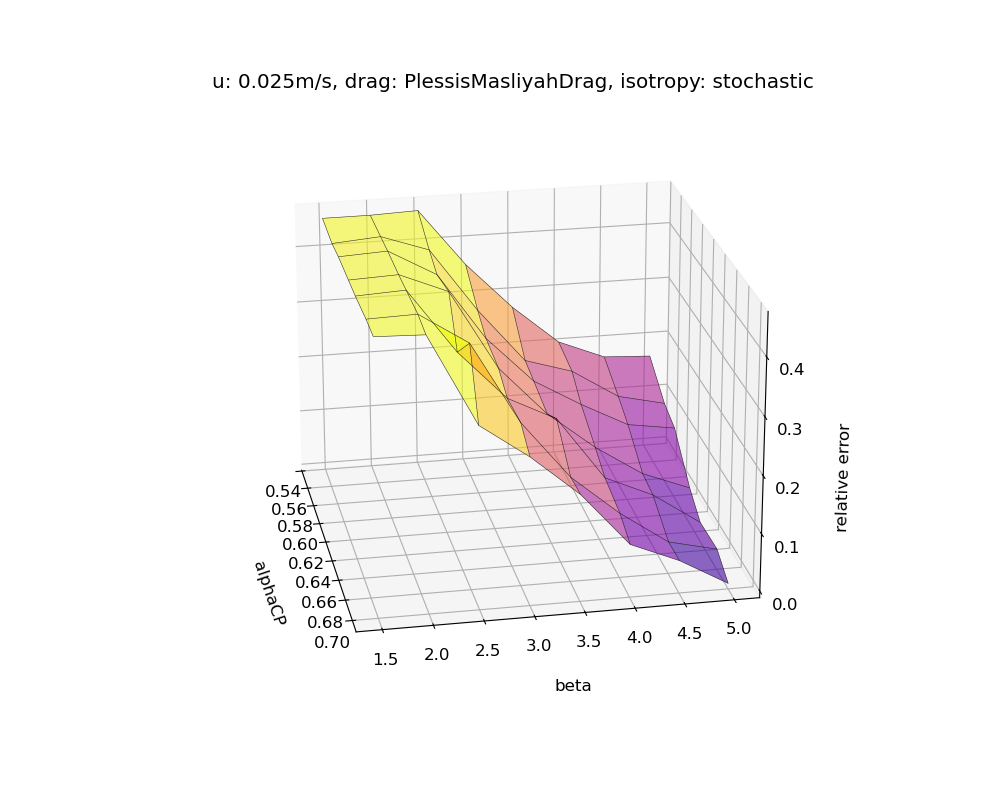
\includegraphics[width = \linewidth, trim = {3.5cm 0 3.5cm 0}, clip]{sections/result/Case 1/Z_height0.025_PlessisMasliyahDrag_stochastic.png}
%         \caption{Relative error of bed height with drag model \lstinline|PlessisMasliyahDrag|, isotropy model \lstinline|stochastic| and inlet velocity $0.025m/s$.}
%     \end{subfigure}
% \end{figure}

% \begin{figure}[h!]
%     \centering
%     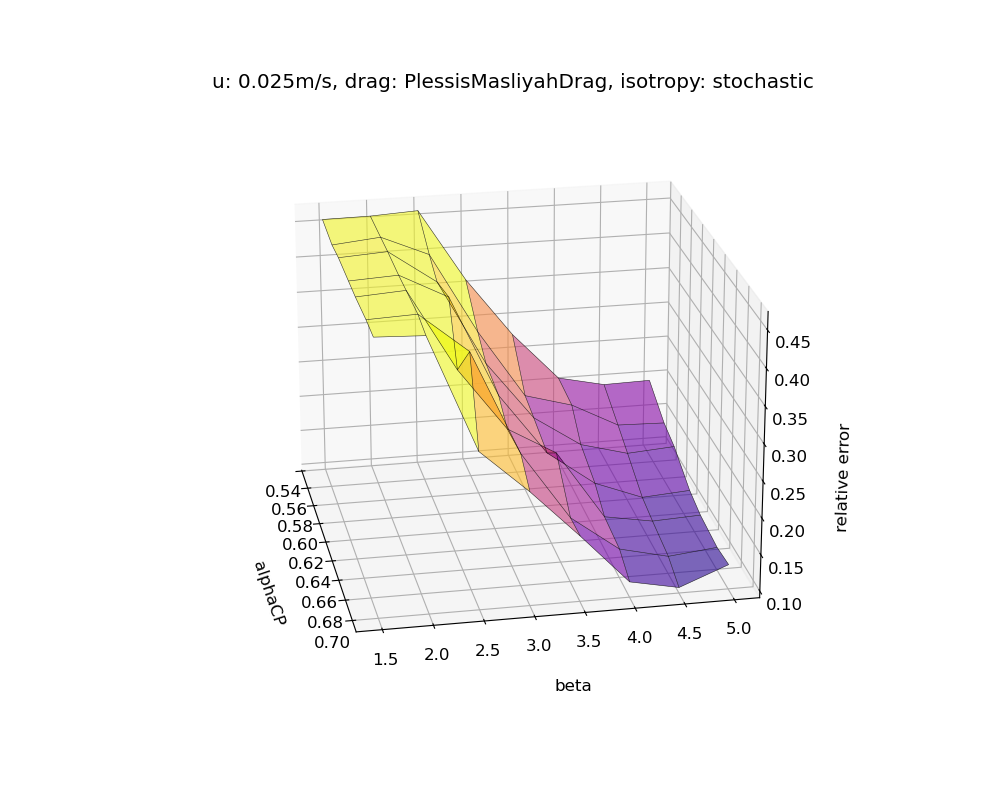
\includegraphics[width=0.5\linewidth, trim = {3.5cm 0 3.5cm 0}, clip]{sections/result/Case 1/Z_both0.025_PlessisMasliyahDrag_stochastic.png}
%     \caption{Combined relative error with drag model \lstinline|PlessisMasliyahDrag|, isotropy model \lstinline|stochastic| and inlet velocity $0.025m/s$, according to equation \eqref{eq:relError}.}
%     \label{fig:placeholder}
% \end{figure}
% \FloatBarrier

\subsection{Case 3: $\beta$ and $P_s$}
In this section we look at the last case where the exponent $\beta$ and the pressure constant $P_s$ are varied. The close pack particle volume fraction $\pvfcp$ is left constant.
We test the parameters for four inlet velocities.
\subsubsection{Inlet velocity $\uf = 0.015 m/s$}

\paragraph{Drag model \lstinline|ErgunWenYu| and isotropy model \lstinline|none|}


\paragraph{Drag model \lstinline|ErgunWenYu| and isotropy model \lstinline|stochastic|}
\paragraph{Drag model \lstinline|PlessisMaliyahDrag| and isotropy model \lstinline|none|}
\paragraph{Drag model \lstinline|PlessisMaliyahDrag| and isotropy model \lstinline|stochastic|}
\fi

In the \MP method the pressure calculated and output is the kinematic pressure, which we multiply by the fluid density $1.2 \operatorname{kg/m^3}$ to get the static pressure.
The kinematic pressure is measured at the top, $P(7.5e-05| 0.005| 0.0497487)$ and the bottom of the grid $P(7.5e-05| 0.005| 0.000251256)$ in the center but not on the boundary.
%\Todo{Punkte einfügen}
The bed height is determined in the simulation by checking if a cell has a fluid volume fraction of less than $0.95$.
We do this in several columns and save for each the top most cell where this is the case.
For the bed height we then average over those values.

In the following we go over all three cases for the velocity of $0.015 \operatorname{m/s}$ and look at the relative error of the pressure, the bed height and the combined relative error define in equation \eqref{eq:relError}.
The results are summarized and discussed in sec \ref{sec:discAndRes}.




\subsection{Case 1: $\pvfcp$ and $\beta$}
%first pressure, second height, third both

First we vary the close pack volume fraction $\pvfcp$ and $\beta$.
The pressure constant $P_s$ is left constant as $P_s = 10$, as set in the \lstinline|Goldschmidt| case.
Here we discuss the inlet velocity $\uf = 0.015 \operatorname{m/s}$. The results of the three remaining velocities are in the Appendix \todo{Appendix einfügen}.

%\subsubsection{Inlet velocity $\uf = 0.015m/s$}

For an inlet velocity $\uf = 0.015m/s$ we expect a bed height of $1.68cm$ and a pressure drop of $140 Pa$.

\paragraph{Drag model \lstinline|ErgunWenYuDrag| and isotropy model \lstinline|none|}
We start by using the \lstinline|ErgunWenYuDrag| drag model and turn off the isotropy model.
The pressure drop is plotted in figure \ref{fig:PDEWYNone0015}. 
The relative error of the pressure drop is minimal for an exponent of $\beta = 4.5$ and close pack particle volume fraction $\pvfcp = 0.7$ with a relative error of $0.23$ before spiking for $\beta = 5$. Possible causes of the high relative error for the pressure drop are discussed in sec \ref{sec:discAndRes}.
The relative error grows for smaller exponents and smaller close pack volume fractions up to $0.30$ at $\beta = 3.0$ and $\pvfcp = 0.55$.
For even smaller $\pvfcp$ the error grows smaller again.



In contrast the minimum relative error for the bed height in figure \ref{fig:BHEWYNone0015} is at $\beta = 5.0$ and $\pvfcp = 0.7$ with a relative error of $0.04$. The error stays largely the same for all parameters and peaks at $0.12$ at $\beta = 1.5$ and $\pvfcp = 0.68$.
Because the relative error from the pressure drop dominates, the overall behavior of the combined relative error is similar to that of the pressure drop, except for slightly smoothed. The lowest relative error aligns with that of the pressure drop and is at $\beta = 4.5$ and $\pvfcp = 0.7$. 

\FloatBarrier
\begin{figure}[h!]
    \centering
    \begin{subfigure}[b]{0.49 \linewidth}
        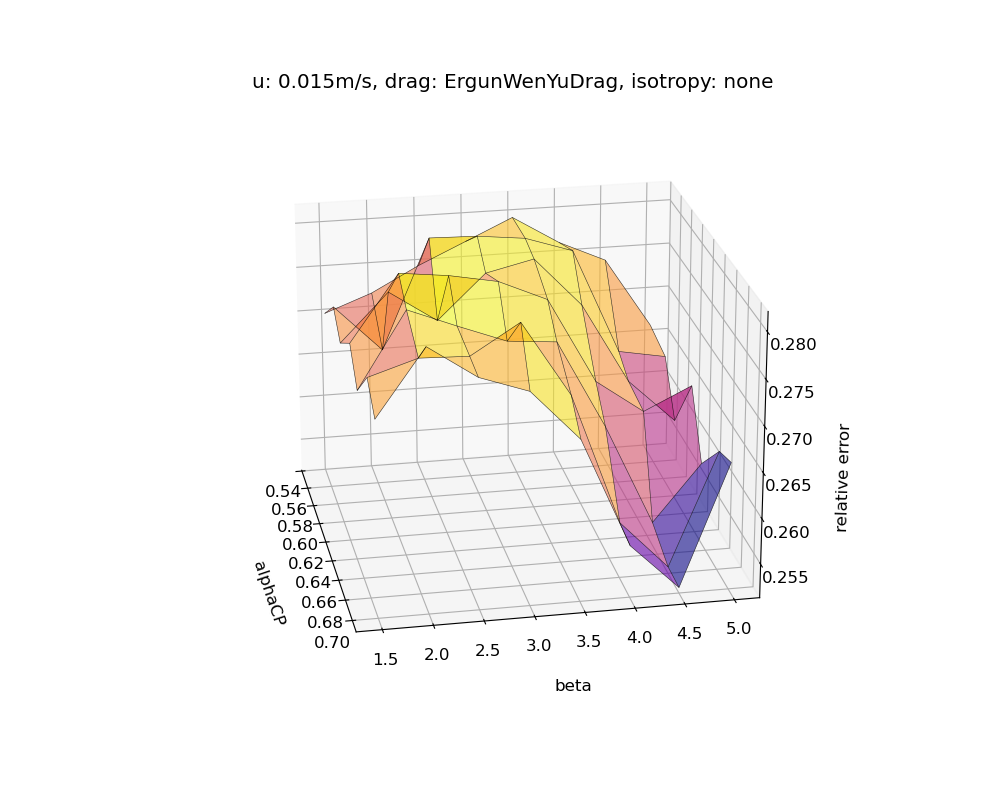
\includegraphics[width = \linewidth, trim = {3.5cm 0 3.5cm 0}, clip]{sections/result/Case1Kin/kin_Z_pres0.015_ErgunWenYuDrag_none.png}
        \caption{Relative error of pressure with drag model \lstinline|ErgunWenYuDrag|, isotropy model \lstinline|none| and inlet velocity $0.015m/s$.}
        \label{fig:PDEWYNone0015}
    \end{subfigure}
    \hfill
    \begin{subfigure}[b]{0.49 \linewidth}
        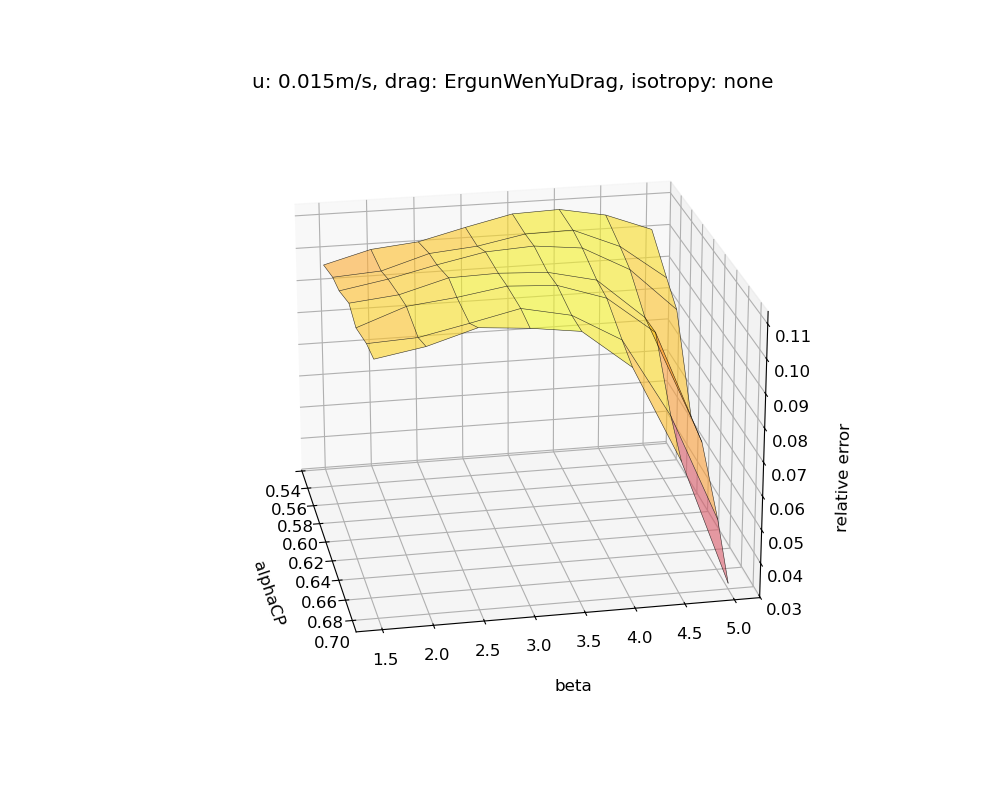
\includegraphics[width = \linewidth, trim = {3.5cm 0 3.5cm 0}, clip]{sections/result/Case1Kin/kin_Z_height0.015_ErgunWenYuDrag_none.png}
        \caption{Relative error of bed height with drag model \lstinline|ErgunWenYuDrag|, isotropy model \lstinline|none| and inlet velocity $0.015m/s$.}
        \label{fig:BHEWYNone0015}
    \end{subfigure}
    \caption{Relative error of the pressure drop (left) and the bed height (right).}
\end{figure}
\todo{Gibt es Meinungen zur Color Map / Plot Style? Der ist am Anfang in Ordnung. Die Plots später meeh}
\begin{figure}[h!]
    \centering
    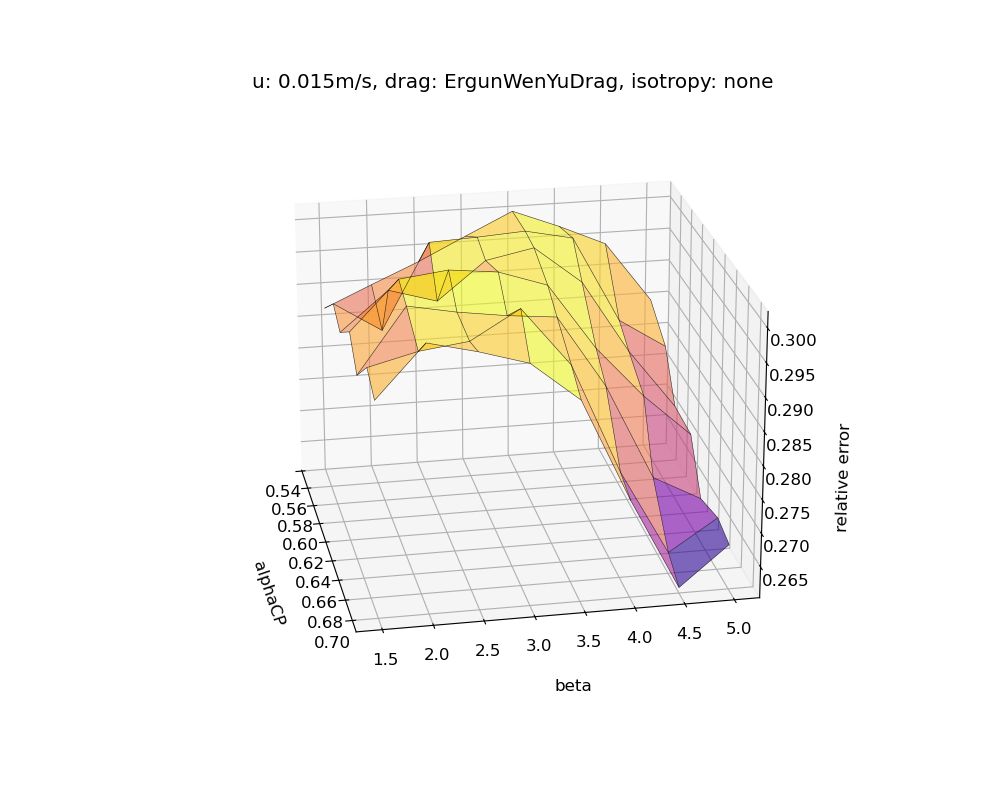
\includegraphics[width=0.5\linewidth, trim = {3.5cm 0 3.5cm 0}, clip]{sections/result/Case1Kin/kin_Z_both0.015_ErgunWenYuDrag_none.png}
    \caption{Combined relative error with drag model \lstinline|ErgunWenYuDrag|, isotropy model \lstinline|none| and inlet velocity $0.015m/s$, according to equation \eqref{eq:relError}.}
    \label{fig:EWYNone0015}
\end{figure}
\FloatBarrier

\paragraph{Drag model \lstinline|ErgunWenYuDrag| and isotropy model \lstinline|stochastic|}
Including the isotropy model in the simulations leads to a vastly different result.
In this case the minimal relative error for the pressure drop of $0.23$ is at $\beta = 2.0$, therefor at the other end of the spectrum. The close pack volume fraction at the minimal relative error is at $\pvf = 0.65$.
The pressure drop peaks at $\beta = 3.0$ and $\pvfcp = 9.55$ with a relative error of $0.30$. 
The bed height is similar to the previous case. Again we see a plateau with a steep slope descending towards high particle volume fractions and exponents.
The minimal relative error can be found at the bottom of the slope at $\beta = 5.0$ and $\pvfcp = 0.7$ with a relative error of $0.04$.
The maximal relative error is at the opposite side with $\beta = 1.5$ and $\pvfcp = 0.68$ and a relative error of $0.12$.
Once again the higher relative error from the pressure drop dominates the overall error.
The parameters of oth the highest and lowest relative overall error coincide with those of the pressure drop.
\FloatBarrier
\begin{figure}[h!]
    \centering
    \begin{subfigure}[b]{0.49 \linewidth}
        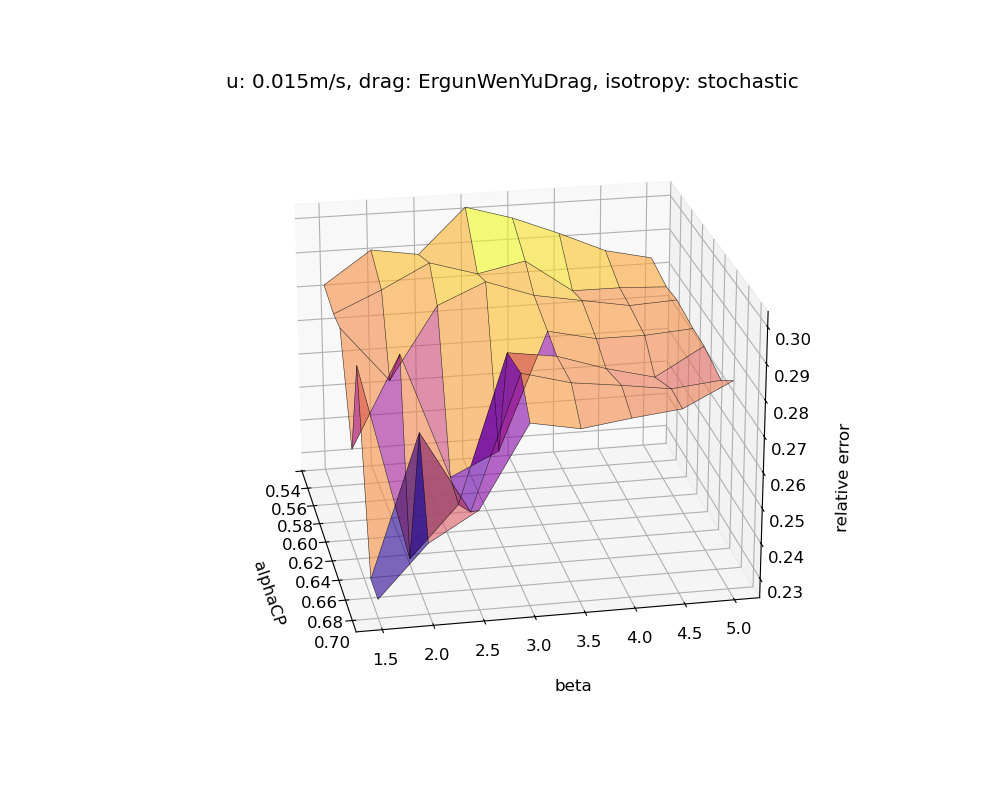
\includegraphics[width = \linewidth, trim = {3.5cm 0 3.5cm 0}, clip]{sections/result/Case1Kin/kin_Z_pres0.015_ErgunWenYuDrag_stochastic.png}
        \caption{Relative error of pressure with drag model \lstinline|ErgunWenYuDrag|, isotropy model \lstinline|stochastic| and inlet velocity $0.015m/s$.}
    \end{subfigure}
    \hfill
    \begin{subfigure}[b]{0.49 \linewidth}
        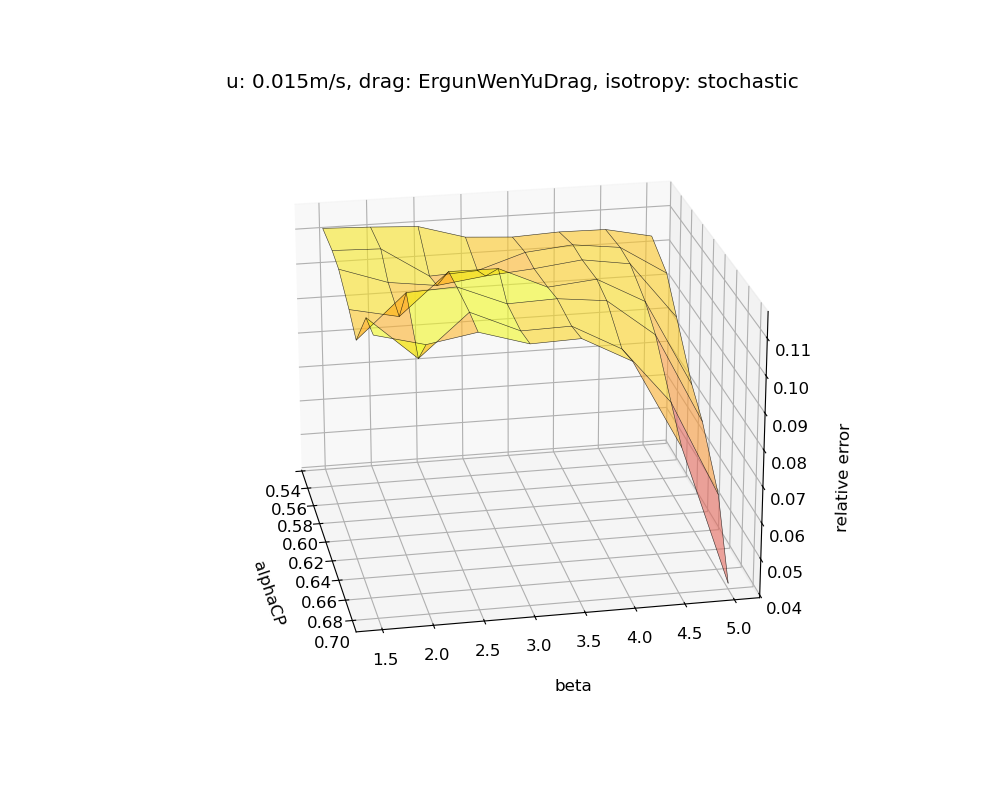
\includegraphics[width = \linewidth, trim = {3.5cm 0 3.5cm 0}, clip]{sections/result/Case1Kin/kin_Z_height0.015_ErgunWenYuDrag_stochastic.png}
        \caption{Relative error of bed height with drag model \lstinline|ErgunWenYuDrag|, isotropy model \lstinline|stochastic| and inlet velocity $0.015m/s$.}
    \end{subfigure}
\end{figure}

\begin{figure}[h!]
    \centering
    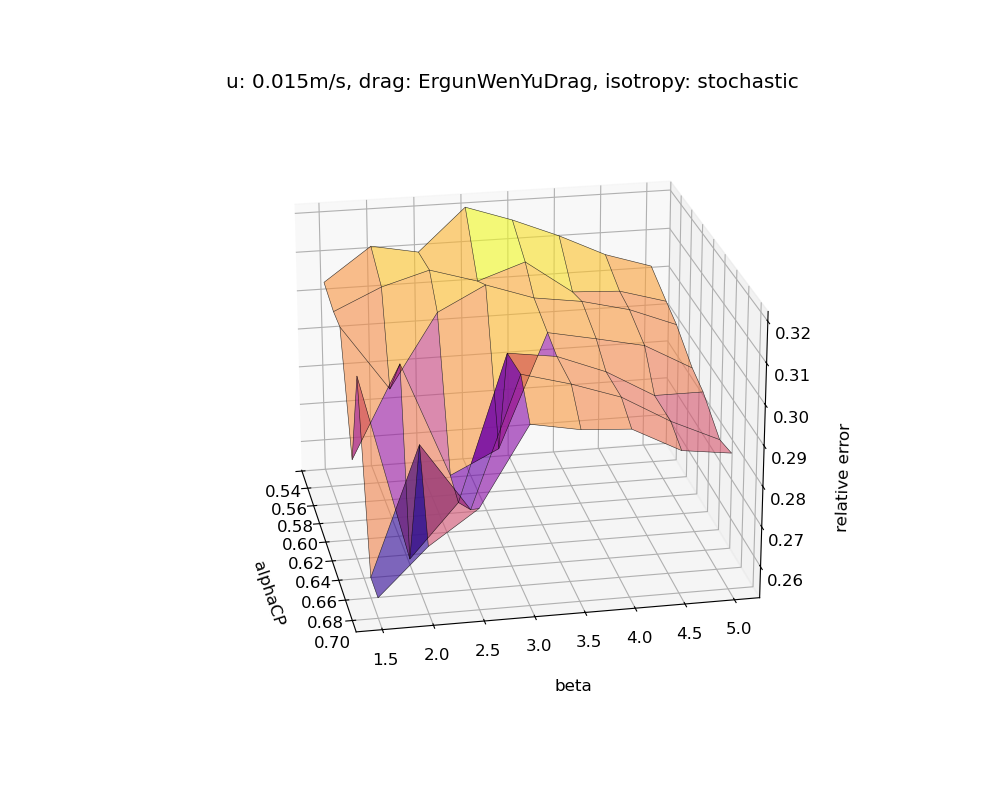
\includegraphics[width=0.5\linewidth, trim = {3.5cm 0 3.5cm 0}, clip]{sections/result/Case1Kin/kin_Z_both0.015_ErgunWenYuDrag_stochastic.png}
    \caption{Combined relative error with drag model \lstinline|ErgunWenYuDrag|, isotropy model \lstinline|stochastic| and inlet velocity $0.015m/s$, according to equation \eqref{eq:relError}.}
    \label{fig:placeholder}
\end{figure}
\FloatBarrier


\paragraph{Drag model \lstinline|PlessisMaliyahDrag| and isotropy model \lstinline|none|}

In the following we swap the \lstinline|ErgunWenYuDrag| model for the \lstinline|PlessisMaliyahDrag| model.
We start again by turning the isotropy model off.

The relative errors for the bed height and the pressure drop show similar trends, both descending for a higher exponent and bigger particle volume fractions.
The pressure drops spikes for $\beta =5$ and $\pvfcp = 0.7$. The minimal relative error for the pressure drop is therefor at $\beta = 4.5$ and $\pvfcp = 0.7$ with a minimal relative error of $0.26$.
The pressure drop error peaks at $\beta = 3.0$ and $\pvfcp = 0.6$ with a marginally higher relative error of $0.29$.
The bed height error again is minimal at $\beta = 5.0$ and $\pvfcp = 0.7$ with a minimal relative error of $0.08$ and peaks at $\beta = 3.5$ and $\pvfcp = 0.58$ with an error of $0.22$.
Both the minimal and maximal bed height error are roughly double that of what they were in the \lstinline|ErgunWenYuDrag| model.

The overall relative error shows the same trend with the minimal relative error at $\pvfcp = 0.68$ and $\beta = 5.0$ of $0.29$ and a maximal relative error at $\pvfcp = 0.6$ and $\beta = 3.0$ of $0.36$.


\FloatBarrier
\begin{figure}[h!]
    \centering
    \begin{subfigure}[b]{0.49 \linewidth}
        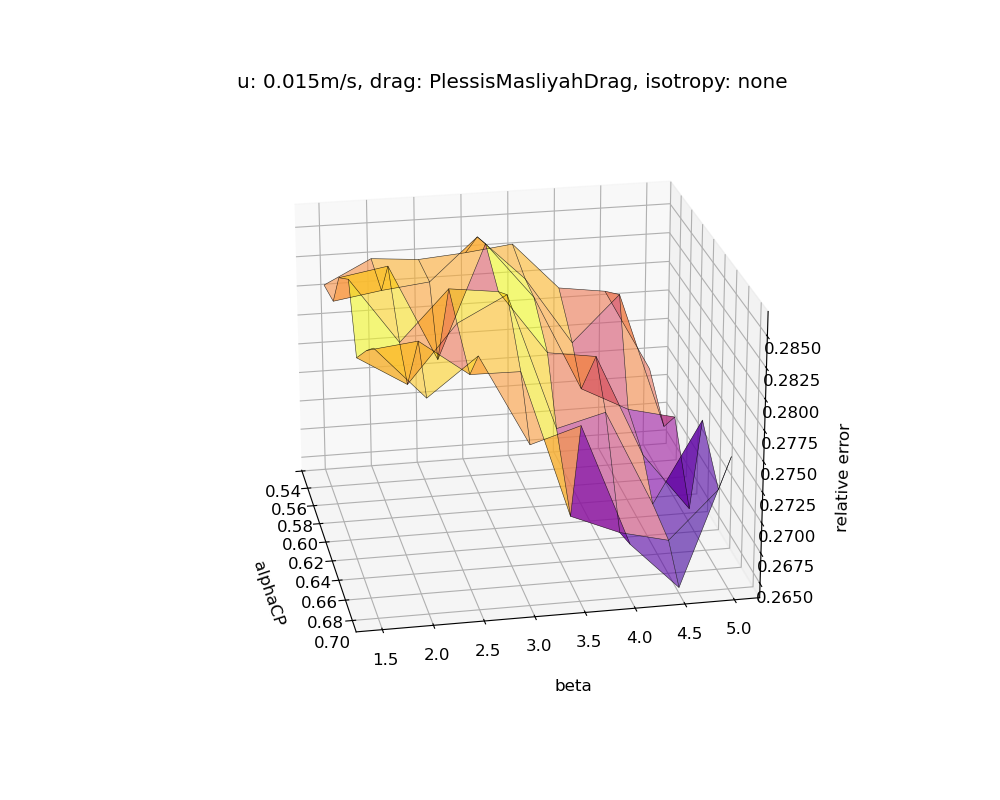
\includegraphics[width = \linewidth, trim = {3.5cm 0 3.5cm 0}, clip]{sections/result/Case1Kin/kin_Z_pres0.015_PlessisMasliyahDrag_none.png}
        \caption{Relative error of pressure with drag model \lstinline|PlessisMasliyahDrag|, isotropy model \lstinline|none| and inlet velocity $0.015m/s$.}
    \end{subfigure}
    \hfill
    \begin{subfigure}[b]{0.49 \linewidth}
        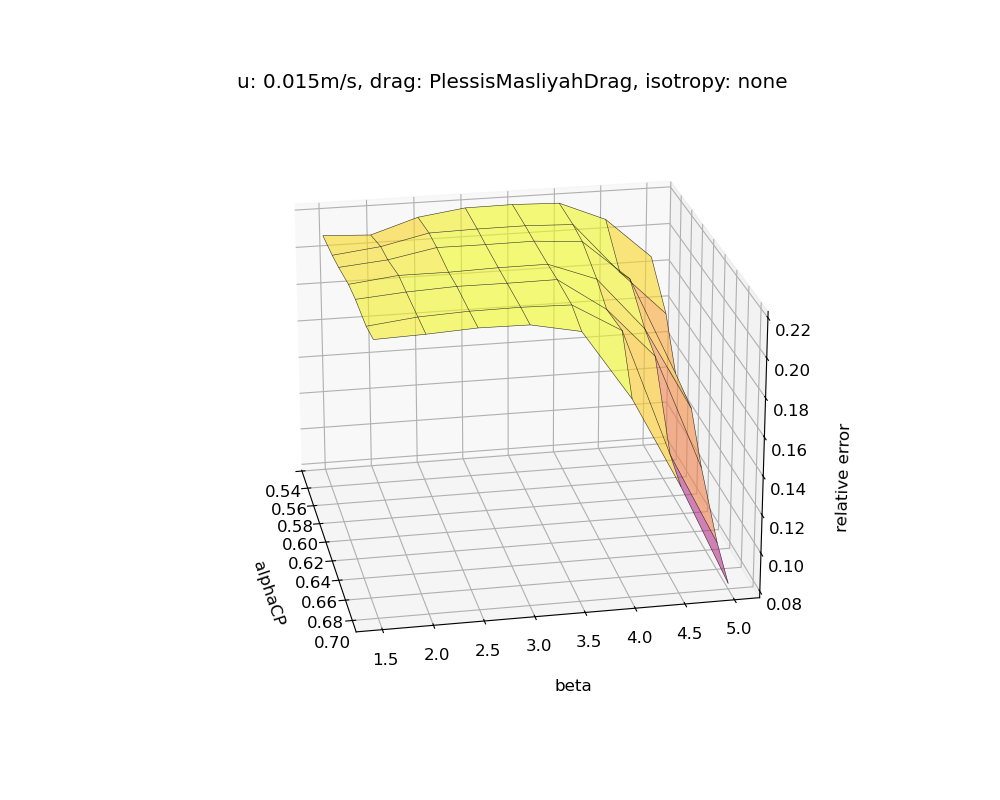
\includegraphics[width = \linewidth, trim = {3.5cm 0 3.5cm 0}, clip]{sections/result/Case1Kin/kin_Z_height0.015_PlessisMasliyahDrag_none.png}
        \caption{Relative error of bed height with drag model \lstinline|PlessisMasliyahDrag|, isotropy model \lstinline|none| and inlet velocity $0.015m/s$.}
    \end{subfigure}
\end{figure}

\begin{figure}[h!]
    \centering
    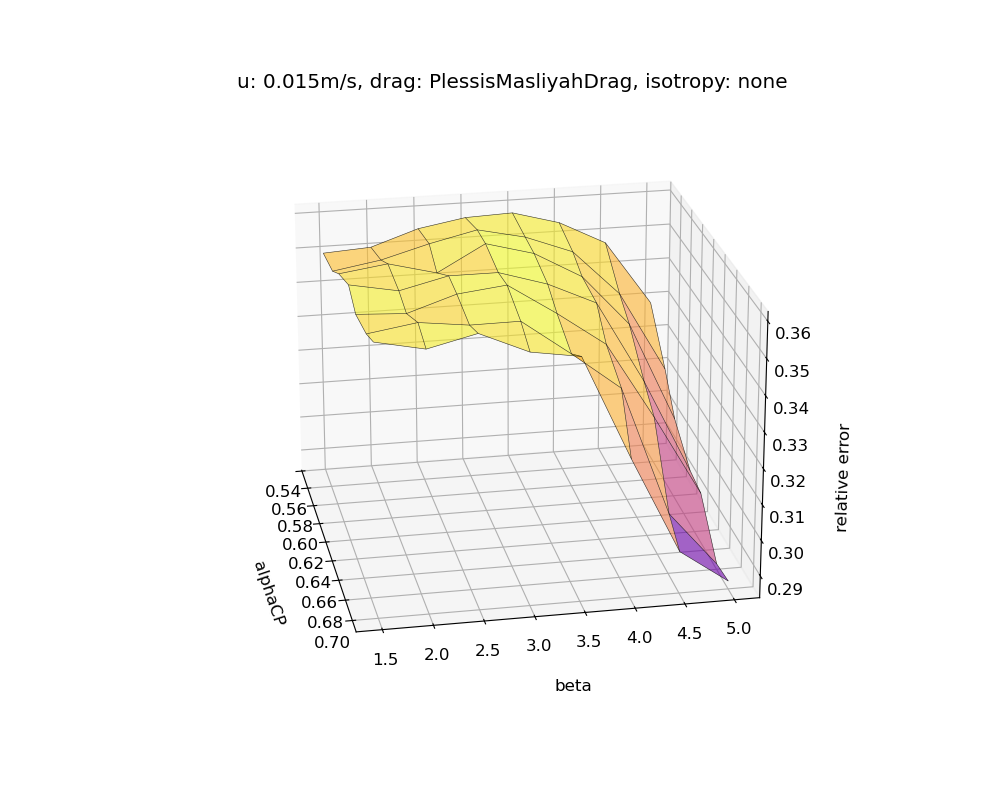
\includegraphics[width=0.5\linewidth, trim = {3.5cm 0 3.5cm 0}, clip]{sections/result/Case1Kin/kin_Z_both0.015_PlessisMasliyahDrag_none.png}
    \caption{Combined relative error with drag model \lstinline|PlessisMasliyahDrag|, isotropy model \lstinline|none| and inlet velocity $0.015m/s$, according to equation \eqref{eq:relError}.}
    \label{fig:placeholder}
\end{figure}
\FloatBarrier



\paragraph{Drag model \lstinline|PlessisMaliyahDrag| and isotropy model \lstinline|stochastic|}

Including the isotropy model in our simulation again switches the impact of the exponent on the pressure drop.
The minimal relative error is at $\beta = 1.5$ and $\pvfcp = 0.68$ with a relative error of $0.24$.
For higher exponents and lower particle volume fraction the relative error is uneven.
The pressure drop has is maximal relative error of $0.29$ at $\beta = 2.0$ and $\pvfcp = 0.55$.
The bed height again plateaus with a maximal error of about $0.22$ at $\beta = 2.5$ and $\pvfcp = 0.7$.


Because the pressure drop error is in a smaller range compared to the bed height the overall relative error is smallest at $\beta = 5.0$ and $\pvfcp = 0.7$ with a relative error of $0.30$.
The bed height dominates the relative error for large exponents and large close pack particle volume fractions and leads to a decline. The error plateaus where both errors are big, therefor at intermediate $\beta$ and declines for smaller exponents analogously to the relative error of the pressure drop.
The maximal error coincides with the parameters of the pressure drop, as the error is larger, at $\pvfcp = 0.55$ and $\beta = 2.0$ and a relative error of $0.36$. 


\FloatBarrier
\begin{figure}[h!]
    \centering
    \begin{subfigure}[b]{0.49 \linewidth}
        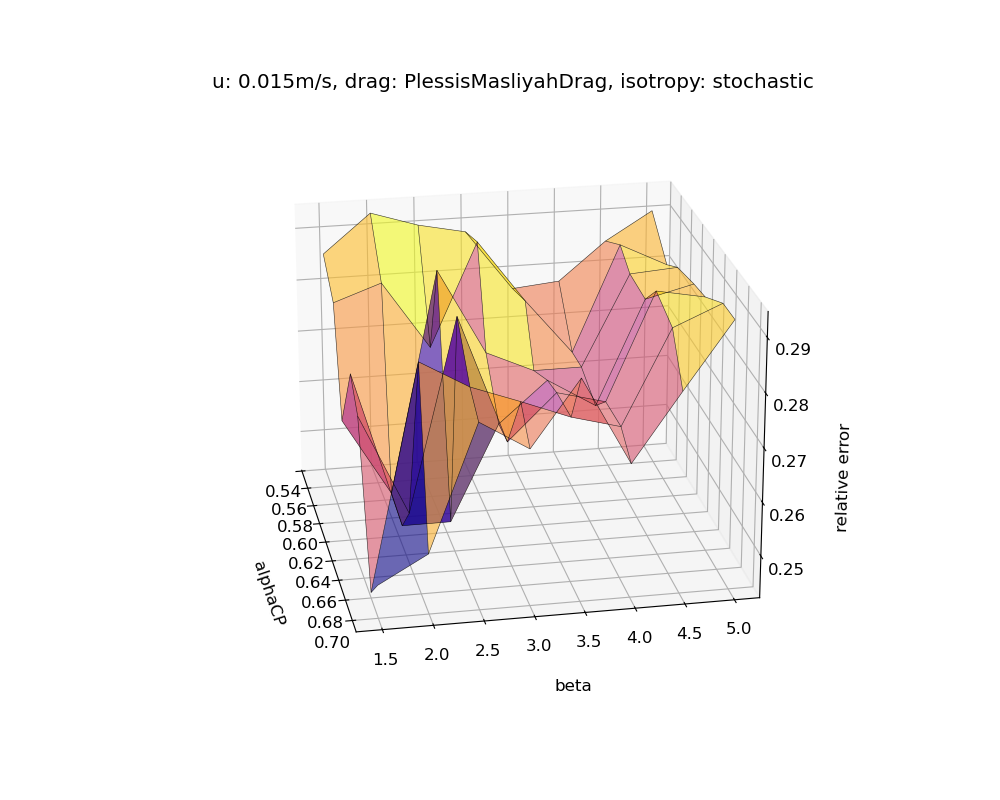
\includegraphics[width = \linewidth, trim = {3.5cm 0 3.5cm 0}, clip]{sections/result/Case1Kin/kin_Z_pres0.015_PlessisMasliyahDrag_stochastic.png}
        \caption{Relative error of pressure with drag model \lstinline|PlessisMasliyahDrag|, isotropy model \lstinline|none| and inlet velocity $0.015m/s$.}
    \end{subfigure}
    \hfill
    \begin{subfigure}[b]{0.49 \linewidth}
        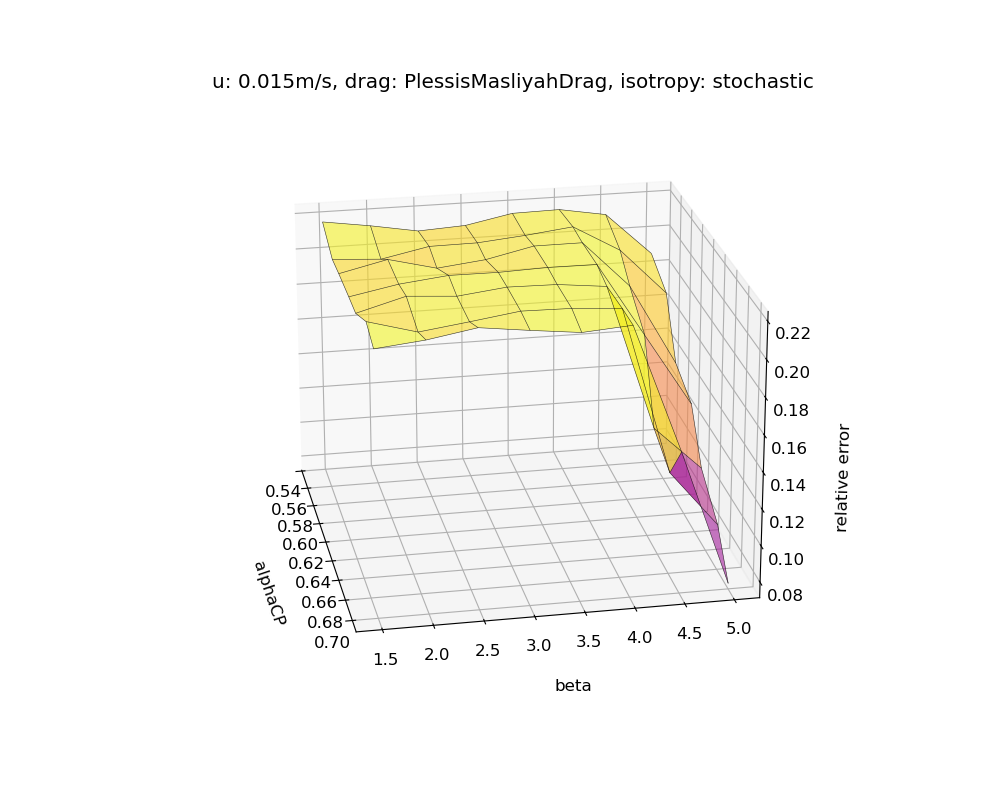
\includegraphics[width = \linewidth, trim = {3.5cm 0 3.5cm 0}, clip]{sections/result/Case1Kin/kin_Z_height0.015_PlessisMasliyahDrag_stochastic.png}
        \caption{Relative error of bed height with drag model \lstinline|PlessisMasliyahDrag|, isotropy model \lstinline|stochastic| and inlet velocity $0.015m/s$.}
    \end{subfigure}
\end{figure}

\begin{figure}[h!]
    \centering
    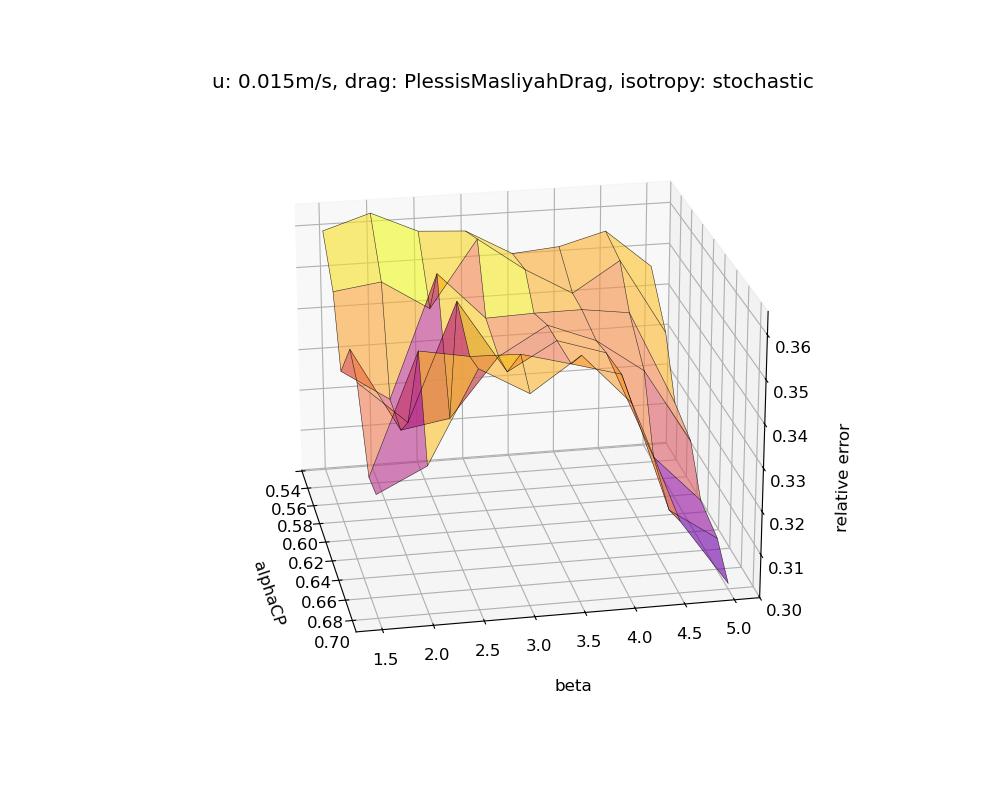
\includegraphics[width=0.5\linewidth, trim = {3.5cm 0 3.5cm 0}, clip]{sections/result/Case1Kin/kin_Z_both0.015_PlessisMasliyahDrag_stochastic.png}
    \caption{Combined relative error with drag model \lstinline|PlessisMasliyahDrag|, isotropy model \lstinline|stochastic| and inlet velocity $0.015m/s$, according to equation \eqref{eq:relError}.}
    \label{fig:placeholder}
\end{figure}
\FloatBarrier

Overall the \lstinline|ErgunWenYuDrag| results in a lower overall error. The bed height plateaus in all four cases. For the \lstinline|ErgunWenYuDra| model at a relative error of about $0.11$ and for the \lstinline|PlessisMasliyahDrag| model at about $0.22$.
In all cases the minimal relative error occurred at higher close pack particle volume fraction. The pressure drop relative error is either at higher beta for no isotropy model or at lower beta for the isotropy model \lstinline|stochastic|. Depending on the bed height the minimal relative error is then sided at either a very high or a very low exponent.


\subsection{Case 2: $\pvfcp$ and $P_s$}
To investigate the impact of the close pack particle volume fraction further we vary it alongside the pressure constant $P_s$.
For now leave the exponent $\beta$ constant.
Once again we only look at the one inlet velocity $\uf = 0.015 m/s$. The plots for the other three cases can be found in the appendix \todo{Appendix erstellen und referenzieren}.


\paragraph{Drag model \lstinline|ErgunWenYuDrag| and isotropy model \lstinline|none|}
Again we start with the \lstinline|ErgunWenYuDrag| model and switch the isotropy model off.
Both the pressure drop error and the bed height error are barely impacted by the different parameters.
The difference in errors is less than $0.02$ for the pressure drop and $0.01$ for the bed height, which is significantly less than in Case 1.
The pressure drop reaches it minimum error of $0.27$ at $P_s = 9.0$ and $\pvfcp = 0.55$. From there we have an incline. The pressure drop error is uneven toward larger close pack particle volume fractions and smaller pressure constants. The error peaks at $0.28$ at $P_s = 6$ and $\pvfcp = 9.58$.
The relative error of the bed height is minimal at $0.01$ at $P_s = 8$ and $\pvfcp = 0.55$ and ascends almost linearly to the maximum error of $0.11$ at $P_s = 6.0$ at $\pvfcp = 0.7$.

The pressure drop error is more than double the bed height error. Therefor the parameters of the minimum relative error of $0.29$ and the parameters of the maximum error of $0.30$ coincide with the parameters of the pressure drop error.

\FloatBarrier
\begin{figure}[h!]
    \centering
    \begin{subfigure}[b]{0.49 \linewidth}
        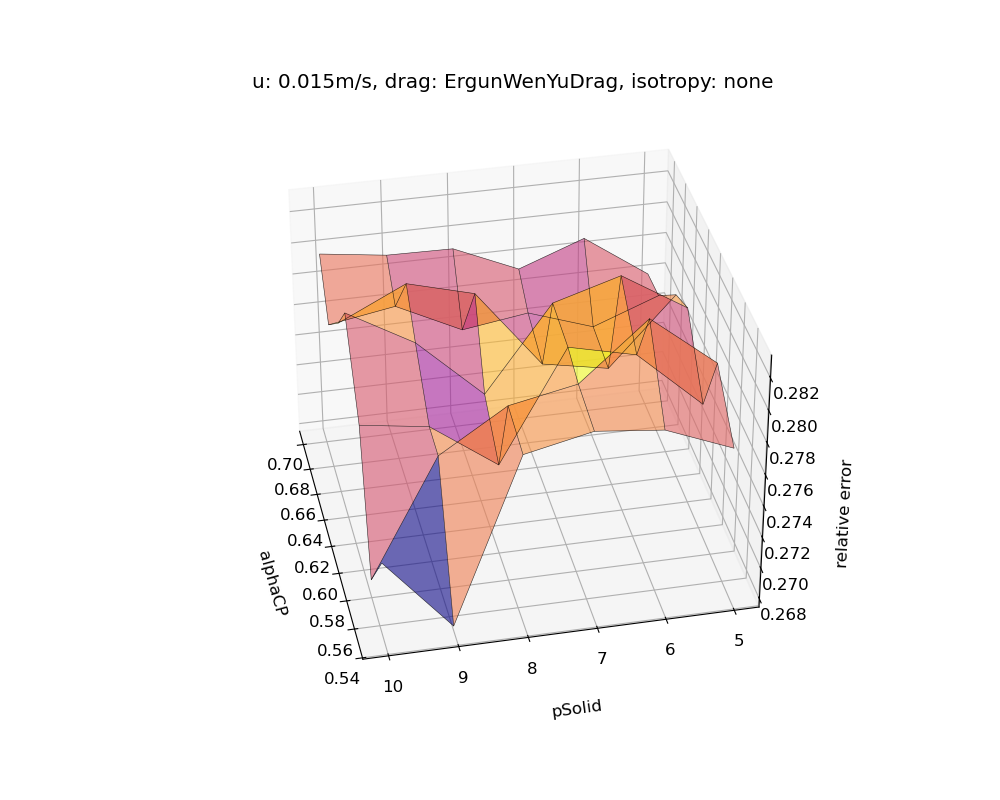
\includegraphics[width = \linewidth, trim = {3.5cm 0 3.5cm 0}, clip]{sections/result/Case2Kin/kin_Z_pres0.015_ErgunWenYuDrag_none.png}
        \caption{Relative error of pressure with drag model \lstinline|ErgunWenYuDrag|, isotropy model \lstinline|none| and inlet velocity $0.015m/s$.}
    \end{subfigure}
    \hfill
    \begin{subfigure}[b]{0.49 \linewidth}
        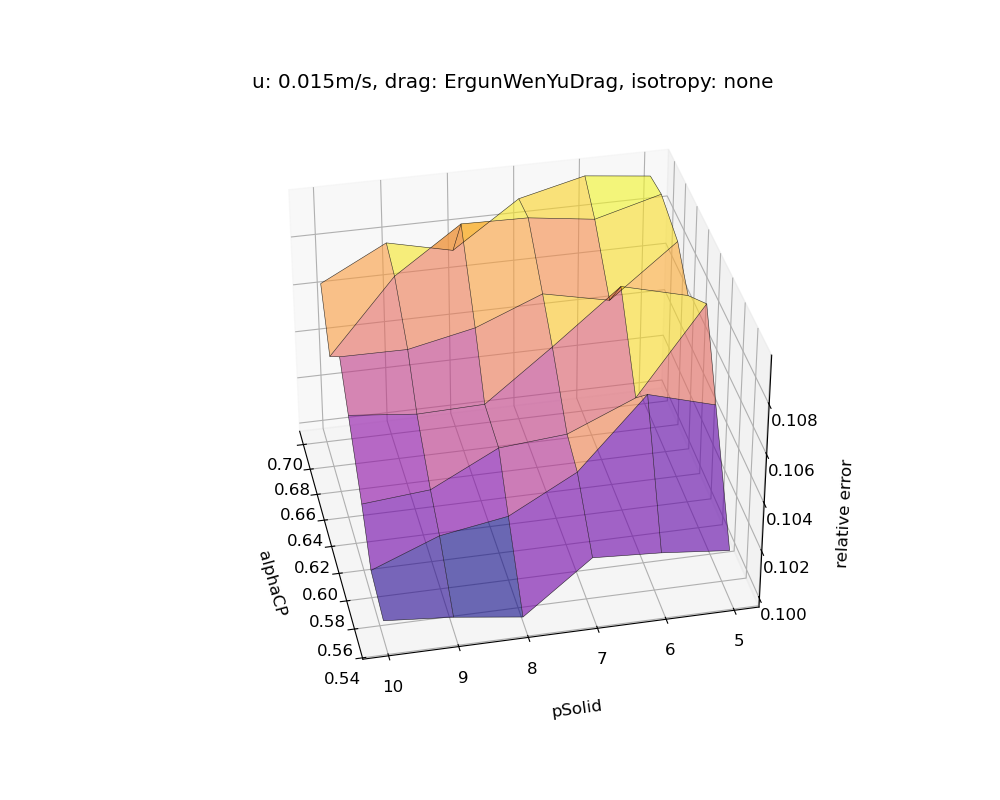
\includegraphics[width = \linewidth, trim = {3.5cm 0 3.5cm 0}, clip]{sections/result/Case2Kin/kin_Z_height0.015_ErgunWenYuDrag_none.png}
        \caption{Relative error of bed height with drag model \lstinline|ErgunWenYuDrag|, isotropy model \lstinline|none| and inlet velocity $0.015m/s$.}
    \end{subfigure}
\end{figure}

\begin{figure}[h!]
    \centering
    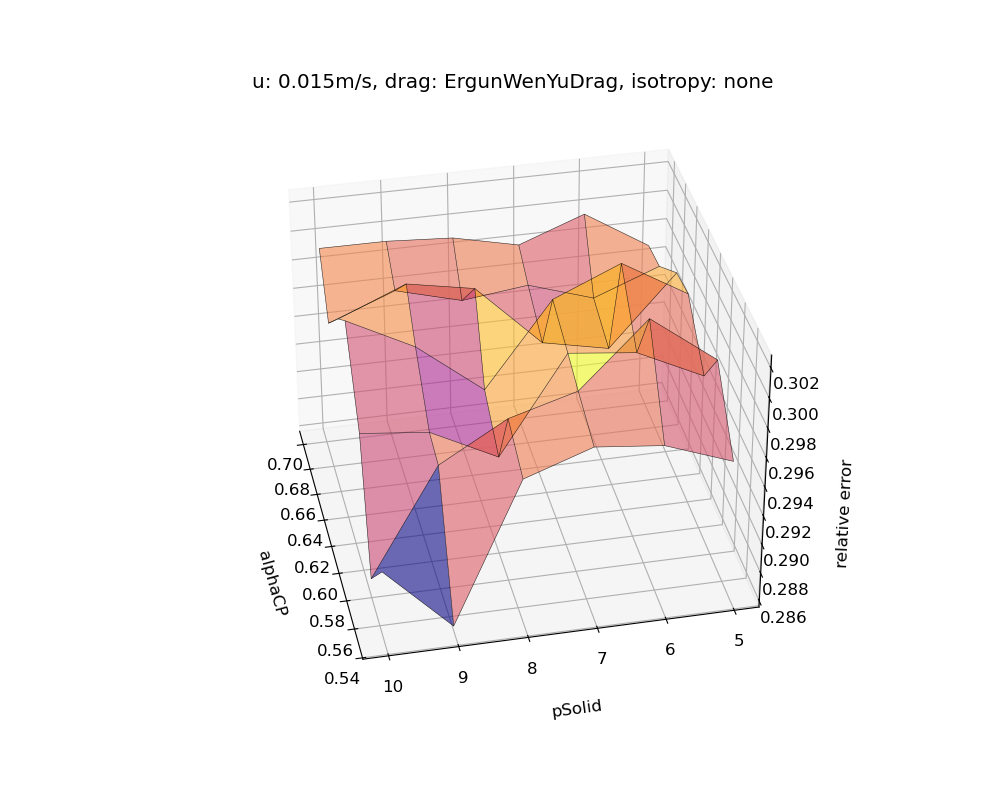
\includegraphics[width=0.5\linewidth, trim = {3.5cm 0 3.5cm 0}, clip]{sections/result/Case2Kin/kin_Z_both0.015_ErgunWenYuDrag_none.png}
    \caption{Combined relative error with drag model \lstinline|ErgunWenYuDrag|, isotropy model \lstinline|none| and inlet velocity $0.015m/s$, according to equation \eqref{eq:relError}.}
    \label{fig:placeholder}
\end{figure}
\FloatBarrier

\paragraph{Drag model \lstinline|ErgunWenYuDrag| and isotropy model \lstinline|stochastic|}
For simulations with the isotropy model the impact of the parameters is more prominent.
The pressure drop error declines for small and large pressure constants and inclines for intermediate values.
The error declines further for larger pressure constants. The minimal error of $0.23$ is at $P_s = 10$ and $\pvfcp = 0.65$. For larger pressure constants the relative error spikes.
The maximum is reached at $P_s = 7.0$ and $\pvf = 0.58$ with an error of $0.3$.

The relative error for the bed height resembles a valley. The error is lowest at $0.10$ for intermediate values of $P_s=8$ and $\pvfcp = 0.63$. The highest value is at the rim with $0.11$ at $P_s = 9.0$ and $\pvfcp = 0.65$.
The difference again here is about $0.01$

Due to the pressure drop error being double that of the bed height error the overall relative error is similar to that of the pressure drop.
The position of the minium error of $0.25$ and of the maximum error of $0.32$ coincide with the pressure drop error.


\FloatBarrier
\begin{figure}[h!]
    \centering
    \begin{subfigure}[b]{0.49 \linewidth}
        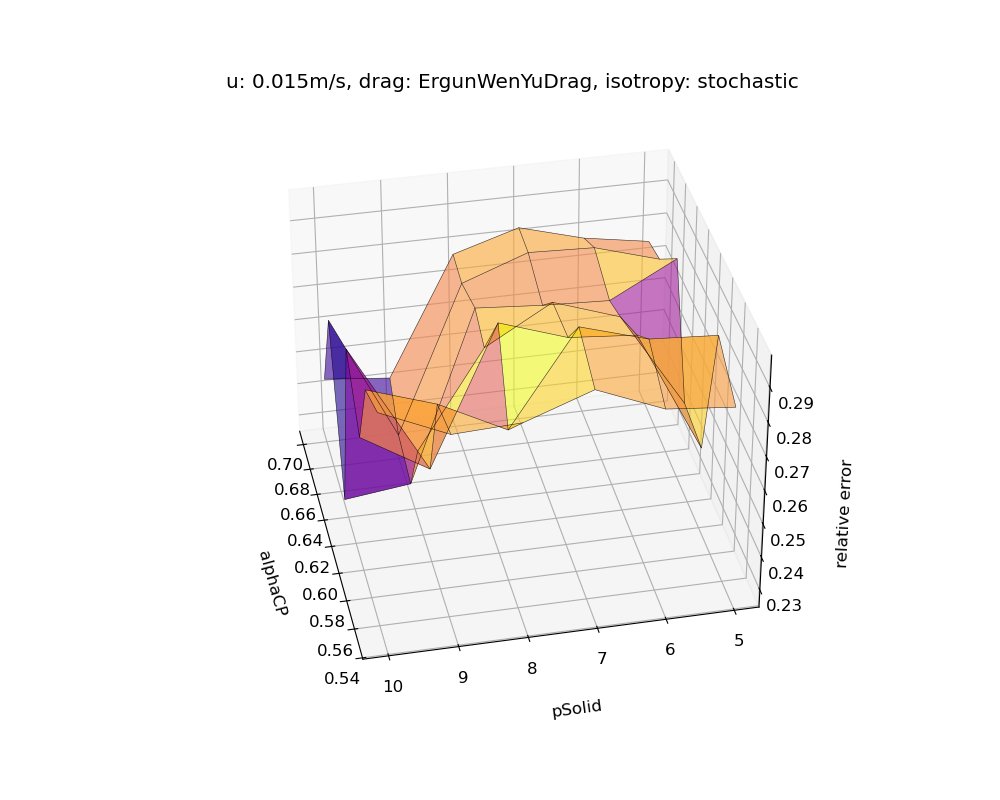
\includegraphics[width = \linewidth, trim = {3.5cm 0 3.5cm 0}, clip]{sections/result/Case2Kin/kin_Z_pres0.015_ErgunWenYuDrag_stochastic.png}
        \caption{Relative error of pressure with drag model \lstinline|ErgunWenYuDrag|, isotropy model \lstinline|stochastic| and inlet velocity $0.015m/s$.}
    \end{subfigure}
    \hfill
    \begin{subfigure}[b]{0.49 \linewidth}
        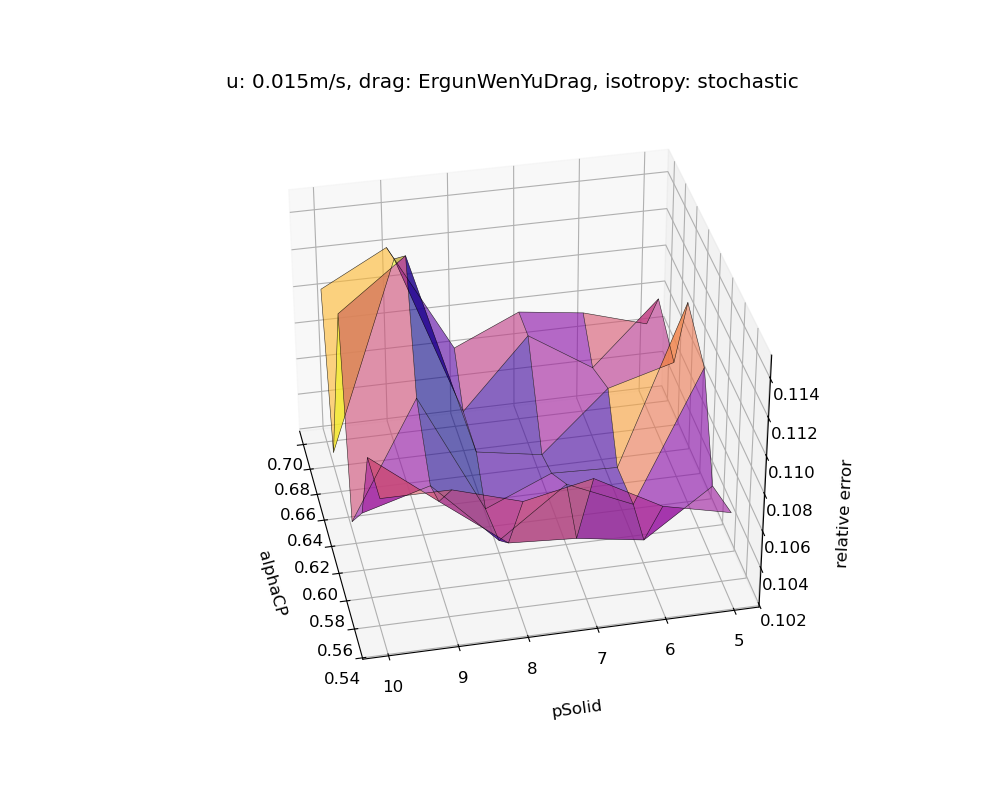
\includegraphics[width = \linewidth, trim = {3.5cm 0 3.5cm 0}, clip]{sections/result/Case2Kin/kin_Z_height0.015_ErgunWenYuDrag_stochastic.png}
        \caption{Relative error of bed height with drag model \lstinline|ErgunWenYuDrag|, isotropy model \lstinline|stochastic| and inlet velocity $0.015m/s$.}
    \end{subfigure}
\end{figure}

\begin{figure}[h!]
    \centering
    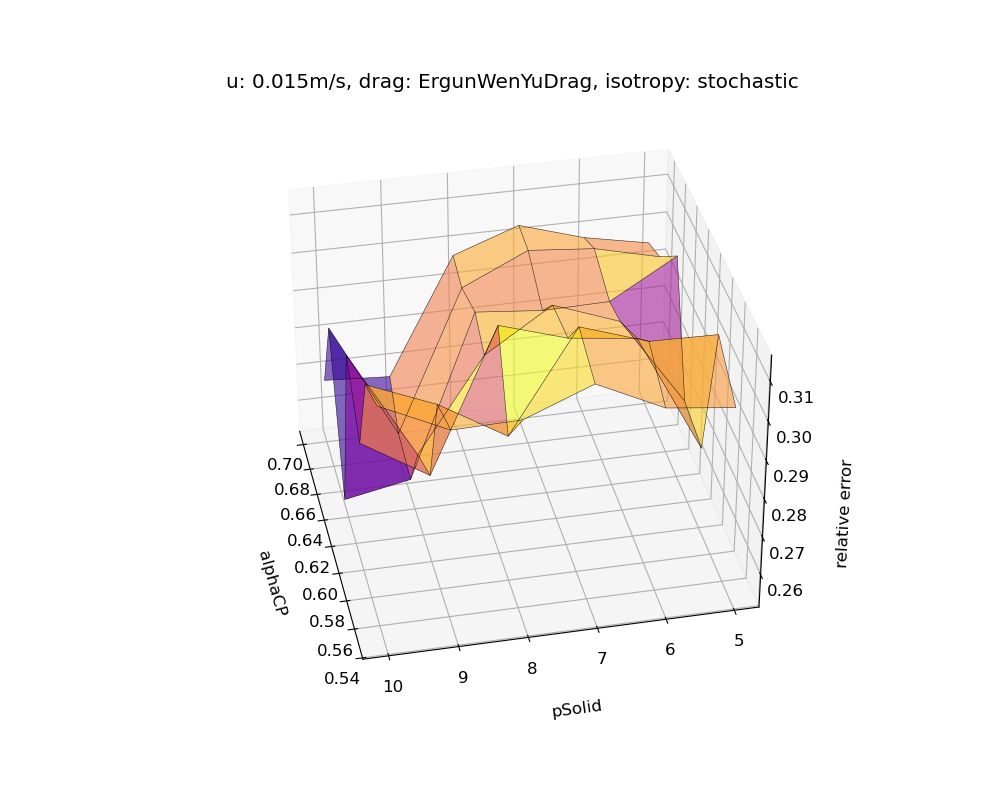
\includegraphics[width=0.5\linewidth, trim = {3.5cm 0 3.5cm 0}, clip]{sections/result/Case2Kin/kin_Z_both0.015_ErgunWenYuDrag_stochastic.png}
    \caption{Combined relative error with drag model \lstinline|ErgunWenYuDrag|, isotropy model \lstinline|stochastic| and inlet velocity $0.015m/s$, according to equation \eqref{eq:relError}.}
    \label{fig:placeholder}
\end{figure}
\FloatBarrier



\paragraph{Drag model \lstinline|PlessisMaliyahDrag| and isotropy model \lstinline|none|}
We change the drag model to \lstinline|PlessisMaliyahDrag|.

The relative error of the pressure drop increases slightly and the relative bed height error nearly doubles compared to the \lstinline|ErgunWenYuDrag| model.

The relative pressure drop error fluctuates in a small range without a clear pattern.
Both the highest and the lowest relative error can be found at intermediate values.
The lowest error is located at $P_s = 8$ and $\pvfcp = 0.58$ with a value of $0.28$ and the highest error is close by at $P_s = 7$ and $\pvfcp = 0.65$ with an error of $0.29$.

The bed height is minimal for $P_s = 10$ and $\pvfcp = 0.55$ with a value of $0.21$. For lower pressure constants and higher close pack particle volume fractions the relative error grows and finally plateaus. 
The largest error is on said plateau at $P_s = 7$ and $\pvfcp = 0.7$ and an error of $0.22$.

The maximum of the overall relative error is located near the peak of the pressure drop at $P_s =8$ and $\pvfcp = 0.55$. The relative error descends in all directions.
The minimum is at $P_s = 8$ and $0.55$ with a minimal error of $0.35$.
The overall error is smaller than the error we observed for the \lstinline|ErgunWenYuDrag| model.

\FloatBarrier
\begin{figure}[h!]
    \centering
    \begin{subfigure}[b]{0.49 \linewidth}
        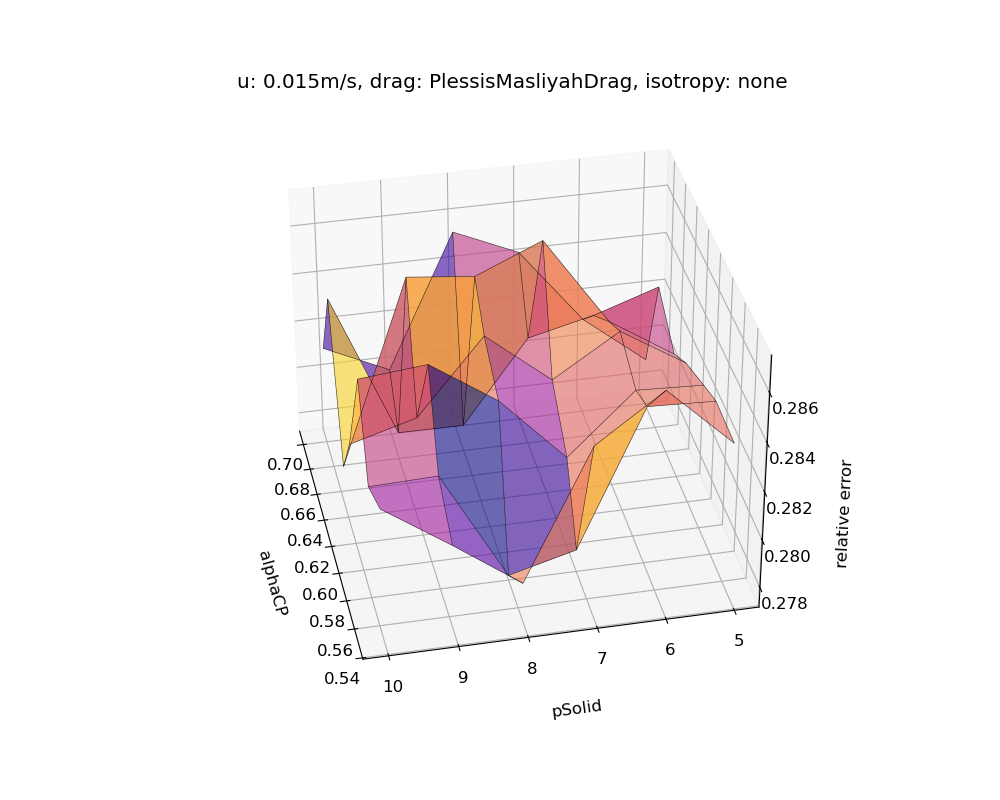
\includegraphics[width = \linewidth, trim = {3.5cm 0 3.5cm 0}, clip]{sections/result/Case2Kin/kin_Z_pres0.015_PlessisMasliyahDrag_none.png}
        \caption{Relative error of pressure with drag model \lstinline|PlessisMasliyahDrag|, isotropy model \lstinline|none| and inlet velocity $0.015m/s$.}
    \end{subfigure}
    \hfill
    \begin{subfigure}[b]{0.49 \linewidth}
        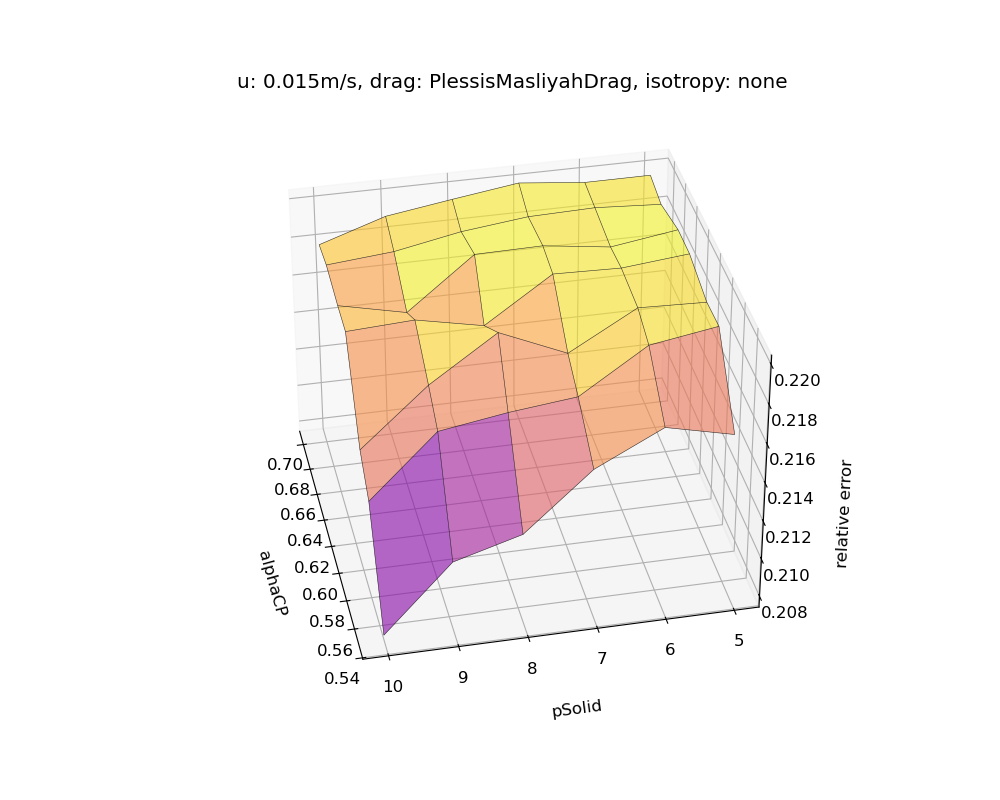
\includegraphics[width = \linewidth, trim = {3.5cm 0 3.5cm 0}, clip]{sections/result/Case2Kin/kin_Z_height0.015_PlessisMasliyahDrag_none.png}
        \caption{Relative error of bed height with drag model \lstinline|PlessisMasliyahDrag|, isotropy model \lstinline|none| and inlet velocity $0.015m/s$.}
    \end{subfigure}
\end{figure}

\begin{figure}[h!]
    \centering
    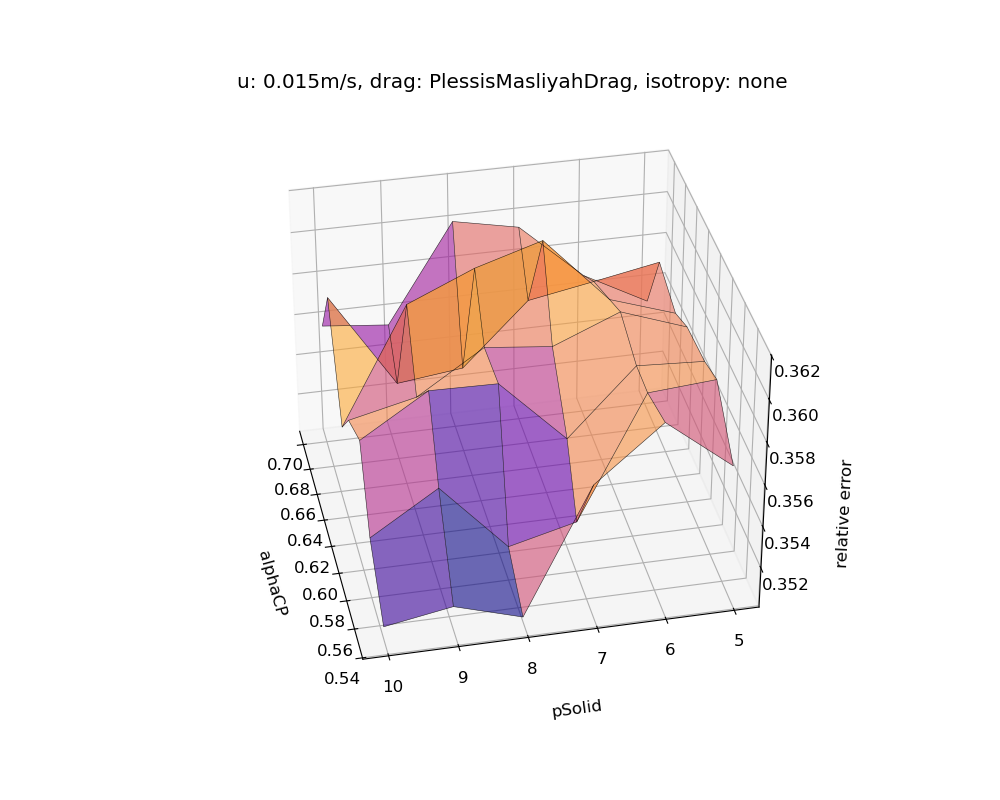
\includegraphics[width=0.5\linewidth, trim = {3.5cm 0 3.5cm 0}, clip]{sections/result/Case2Kin/kin_Z_both0.015_PlessisMasliyahDrag_none.png}
    \caption{Combined relative error with drag model \lstinline|PlessisMasliyahDrag|, isotropy model \lstinline|none| and inlet velocity $0.015m/s$, according to equation \eqref{eq:relError}.}
    \label{fig:placeholder}
\end{figure}
\FloatBarrier



\paragraph{Drag model \lstinline|PlessisMaliyahDrag| and isotropy model \lstinline|stochastic|}

Turning the isotropy model back on the error range of the pressure drop once again increases.
The pressure drop error fluctuates without a clear pattern. The maximum error of  $0.24$ is attained at $P_s = 8$ and $\pvfcp = 0.63$ and the minimum of $0.29$ at $P_s = 10$ and $\pvfcp = 0.55$.

Although the relative error of the bed height is the same range as with the previous model the behavior of the error is different.
The bed height relative error grows for small pressure constants and large close pack volume fractions. Toward the opposite side a we can observe a valley that spikes again for smaller close pack particle volume fractions.
The minimum error of $0.21$ is at $P_s = 10$ and $\pvfcp = 0.58$ and the maximum error is at $P_s = 5$ and $\pvfcp = 0.65$ with an error of $0.22$.


Similarly to the pressure drop error the overall relative error fluctuates without an identifiable pattern.
The minimal error of $0.33$ occurs at $P_s = 10$ and $\pvfcp = 0.63$.
We observe a maximal error of $0.36$ at $P_s = 10$ and $\pvfcp = 0.55$.

\FloatBarrier
\begin{figure}[h!]
    \centering
    \begin{subfigure}[b]{0.49 \linewidth}
        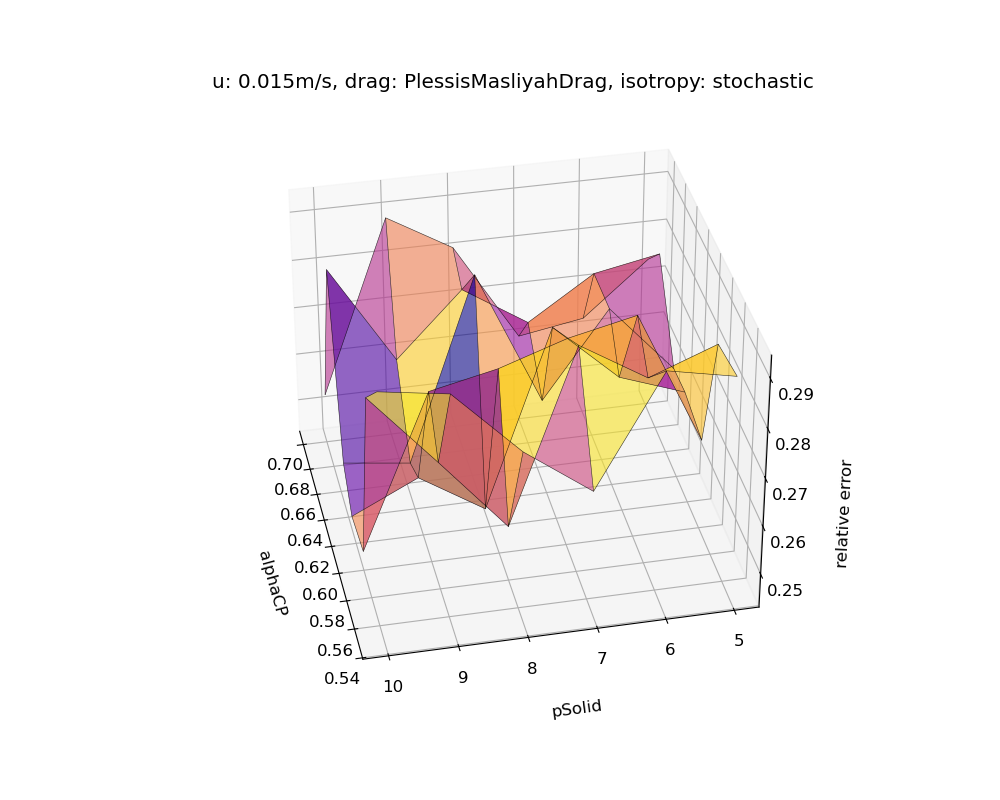
\includegraphics[width = \linewidth, trim = {3.5cm 0 3.5cm 0}, clip]{sections/result/Case2Kin/kin_Z_pres0.015_PlessisMasliyahDrag_stochastic.png}
        \caption{Relative error of pressure with drag model \lstinline|PlessisMasliyahDrag|, isotropy model \lstinline|none| and inlet velocity $0.015m/s$.}
    \end{subfigure}
    \begin{subfigure}[b]{0.49 \linewidth}
        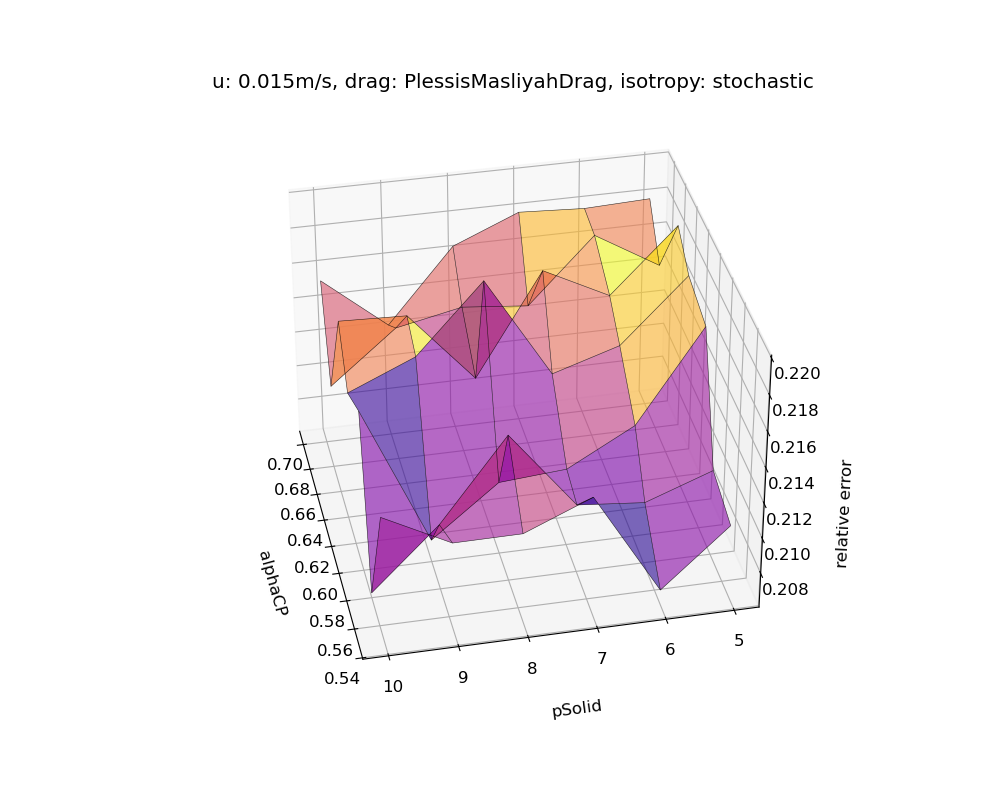
\includegraphics[width = \linewidth, trim = {3.5cm 0 3.5cm 0}, clip]{sections/result/Case2Kin/kin_Z_height0.015_PlessisMasliyahDrag_stochastic.png}
        \caption{Relative error of bed height with drag model \lstinline|PlessisMasliyahDrag|, isotropy model \lstinline|stochastic| and inlet velocity $0.015m/s$.}
    \end{subfigure}
\end{figure}

\begin{figure}[h!]
    \centering
    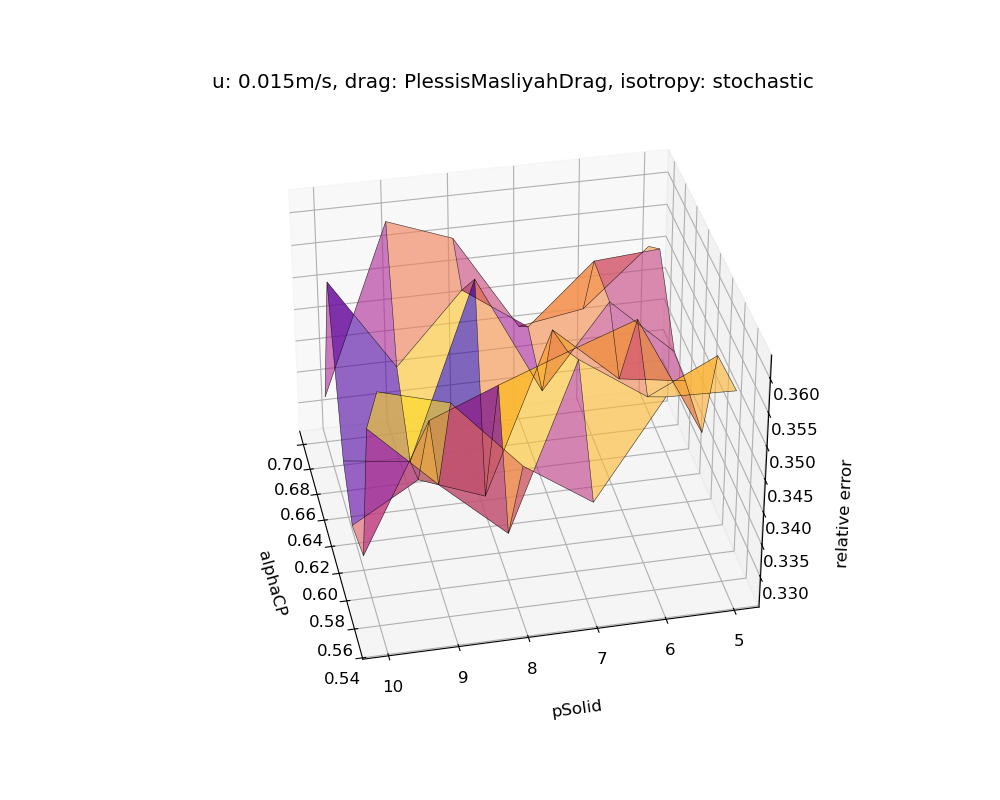
\includegraphics[width=0.5\linewidth, trim = {3.5cm 0 3.5cm 0}, clip]{sections/result/Case2Kin/kin_Z_both0.015_PlessisMasliyahDrag_stochastic.png}
    \caption{Combined relative error with drag model \lstinline|PlessisMasliyahDrag|, isotropy model \lstinline|stochastic| and inlet velocity $0.015m/s$, according to equation \eqref{eq:relError}.}
    \label{fig:placeholder}
\end{figure}
\FloatBarrier


Overall varying both the close pack volume fraction and the pressure constant do not yield a substantial difference in error.
The impact of the parameters is bigger in \lstinline|PlessisMaliyahDrag| but the minimal errors are smaller in the \lstinline|ErgunWenYuDrag| model. The error of the bed height nearly doubles for the former model.

\subsection{Case 3: $\beta$ and $P_s$}
We study the remaining parameter combination by varying the exponent $\beta$ and the pressure constant $P_s$.
We leave the close pack particle volume fraction constant at $\pvfcp = 0.65$.
The inlet velocity is set to $\uf = 0.015 \operatorname{m/s}$ here. Investigations for different velocities can be found at \todo{Apendixxxxxxxxxx}.

\paragraph{Drag model \lstinline|ErgunWenYu| and isotropy model \lstinline|none|}

Starting off we use the \lstinline|ErgunWenYuDrag| model and switch the isotropy model off.
The pressure drop spikes for a high exponent and a low pressure constant. At $\beta = 5$ and $P_s = 5$ the relative error reaches the maximum of $0.31$.
This is followed by a sharp decline with a minimum relative error at $\beta = 4.5$ and $P_s = 10$ of $0.25$.
The relative error rises for lower exponents and higher pressure
constants.

The relative error of the bed height plateaus for lower exponents and higher pressure constants. 
The maximum is located on the plateau at $\beta = 3$ and $P_s = 8$ with a maximum of $0.19$.
The plateau then drops off toward the minimum of $0.08$ at $P_s = 5$ and $\beta = 5$.
Compared to the previous case the parameters modify the range of the relative error more.

Combining the two errors we have a maximum error of  $0.34$  at $\beta = 2$ and $P_s = 9$. 
The relative error drops sharply for lower exponents and pressure constants.
The minimum relative error of $0.29$ is reached at $\beta = 4.5$ and $P_s = 5$.
 For $\beta = 5$ and $P_s = 5$ the error spikes again.
\ifcode
\begin{lstlisting}
    6
5
4.5
10.0
0.25384548817335245
7
0
5.0
5.0
0.307017811336452
0.015_ErgunWenYuDrag_none.png
7
0
5.0
5.0
0.08143407304523503
3
3
3.0
8.0
0.18651156917831999
0.015_ErgunWenYuDrag_none.png
6
0
4.5
5.0
0.2917035307552794
1
4
2.0
9.0
0.3364036991892013
0.015_ErgunWenYuDrag_none.png

\end{lstlisting}
\fi
\FloatBarrier
\begin{figure}[h!]
    \centering
    \begin{subfigure}[b]{0.49 \linewidth}
        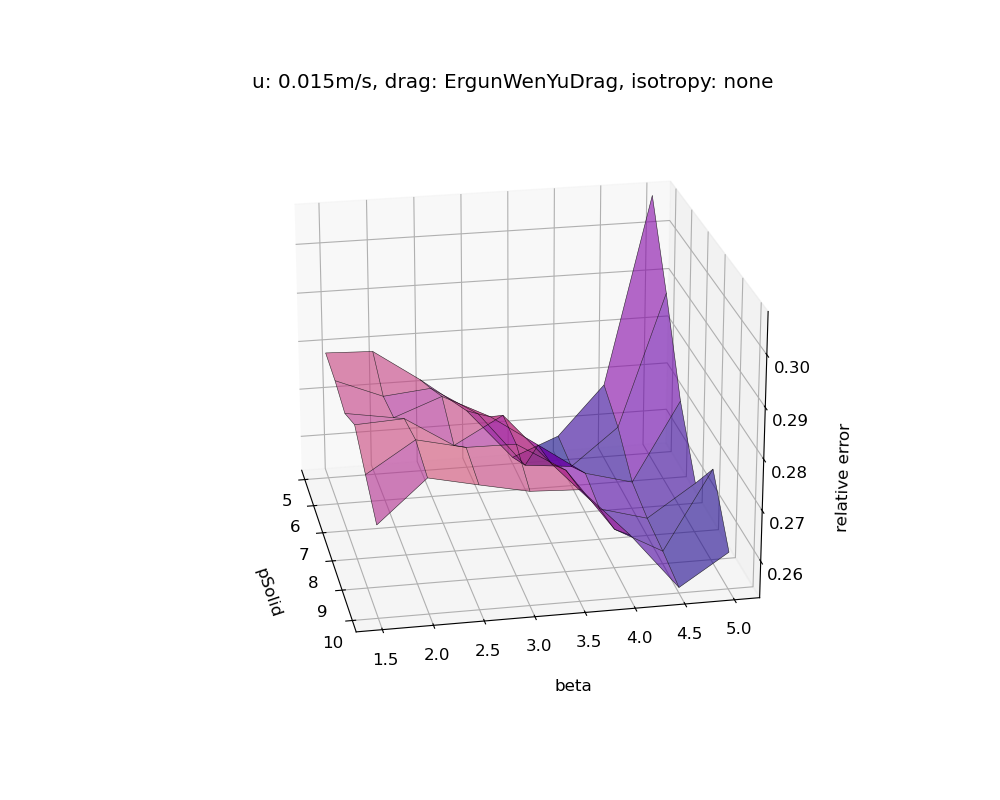
\includegraphics[width = \linewidth, trim = {3.5cm 0 3.5cm 0}, clip]{sections/result/Case3Kin/kin_Z_pres0.015_ErgunWenYuDrag_none.png}
        \caption{Relative error of pressure with drag model \lstinline|ErgunWenYuDrag|, isotropy model \lstinline|none| and inlet velocity $0.015m/s$.}
    \end{subfigure}
    \hfill
    \begin{subfigure}[b]{0.49 \linewidth}
        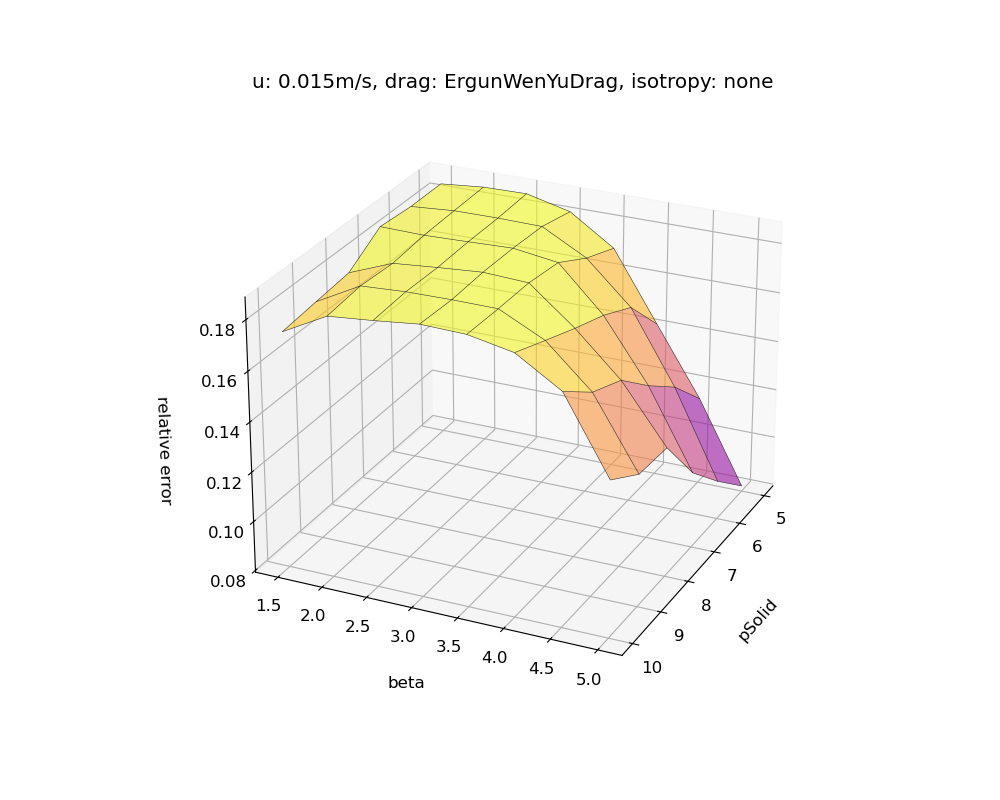
\includegraphics[width = \linewidth, trim = {3.5cm 0 3.5cm 0}, clip]{sections/result/Case3Kin/kin_Z_height0.015_ErgunWenYuDrag_none.png}
        \caption{Relative error of bed height with drag model \lstinline|ErgunWenYuDrag|, isotropy model \lstinline|none| and inlet velocity $0.015m/s$.}
    \end{subfigure}
\end{figure}

\begin{figure}[h!]
    \centering
    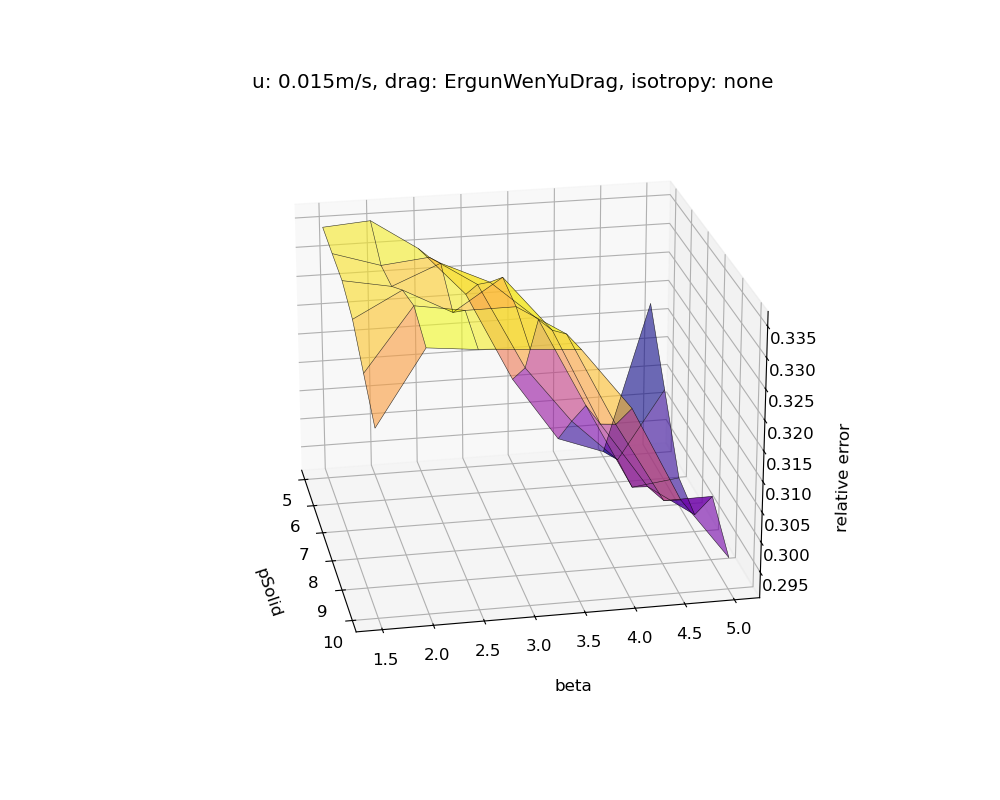
\includegraphics[width=0.5\linewidth, trim = {3.5cm 0 3.5cm 0}, clip]{sections/result/Case3Kin/kin_Z_both0.015_ErgunWenYuDrag_none.png}
    \caption{Combined relative error with drag model \lstinline|ErgunWenYuDrag|, isotropy model \lstinline|none| and inlet velocity $0.015m/s$, according to equation \eqref{eq:relError}.}
    \label{fig:placeholder}
\end{figure}
\FloatBarrier

\paragraph{Drag model \lstinline|ErgunWenYu| and isotropy model \lstinline|stochastic|}

We switich the isotropy model back on.
The pressure drop error plateaus for intermediate values of the parameters.
For low exponents and and high pressure constants the error drops to $0.23$ at $\beta = 2$ and $P_s = 10$.
On the opposite end of the parameters the relative error spikes to $0.34$ at $\beta = 5$ and $P_s = 5$.


The relative error of the bed height shows a similar behavior compared to the simulation without a damping model.
The plateau for lower exponents and pressure constants contains the maximum of $0.18$ at $\beta = 2$ and $P_s = 9$.
The error falls for higher exponents and lower pressure constants.
The lowest relative error is at $\beta = 5$ and $P_s = 5$ with $0.08$.

The downward trend of the bed height error for higher exponents and lower pressure constants is passed on to the combined relative error.
Both spikes of the pressure drop relative error is also visible in the overall error.
The largest error is located at the upward spike with an error of $0.35$ at $P_s = 5$ and $\beta = 5$.
The lowest error is located at the downward spike with a relative error of $0.29$ at $\beta = 2$ and $P_s = 10$.

\ifcode
\begin{lstlisting}
    1
5
2.0
10.0
0.2262068209333094
7
0
5.0
5.0
0.3394784947177058
0.015_ErgunWenYuDrag_stochastic.png
7
0
5.0
5.0
0.08174973957511283
1
4
2.0
9.0
0.1867088607594936
0.015_ErgunWenYuDrag_stochastic.png
1
5
2.0
10.0
0.2933082414847259
7
0
5.0
5.0
0.34918285796470333
\end{lstlisting}
\fi

\FloatBarrier
\begin{figure}[h!]
    \centering
    \begin{subfigure}[b]{0.49 \linewidth}
        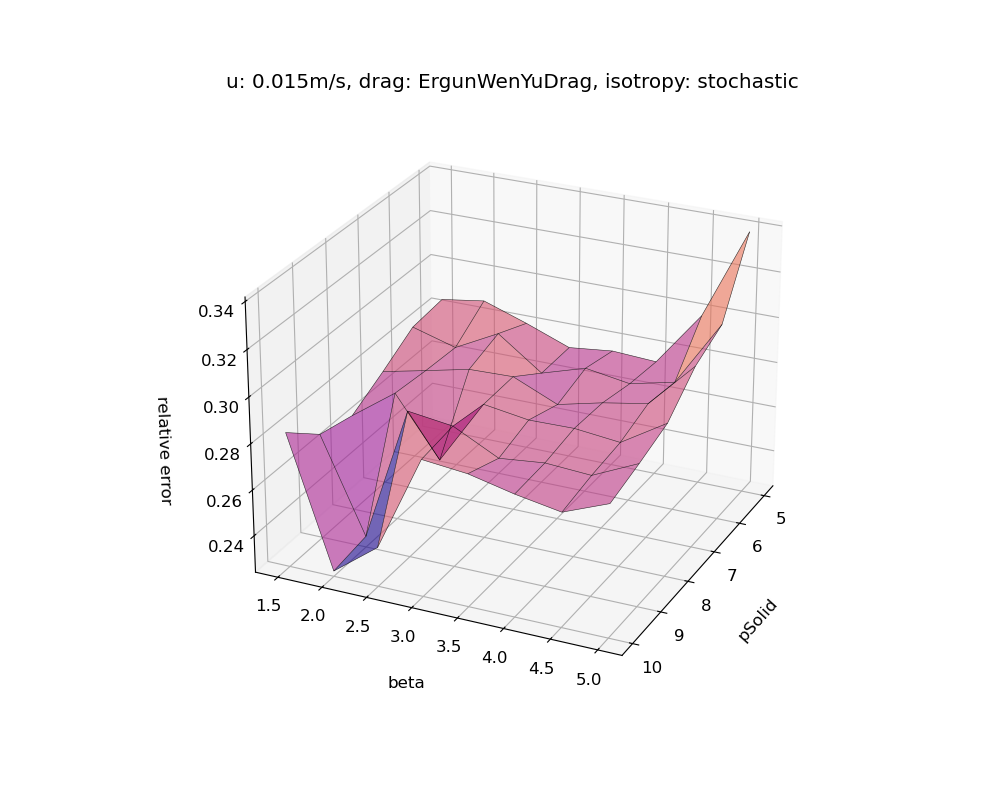
\includegraphics[width = \linewidth, trim = {3.5cm 0 3.5cm 0}, clip]{sections/result/Case3Kin/kin_Z_pres0.015_ErgunWenYuDrag_stochastic.png}
        \caption{Relative error of pressure with drag model \lstinline|ErgunWenYuDrag|, isotropy model \lstinline|stochastic| and inlet velocity $0.015m/s$.}
    \end{subfigure}
    \hfill
    \begin{subfigure}[b]{0.49 \linewidth}
        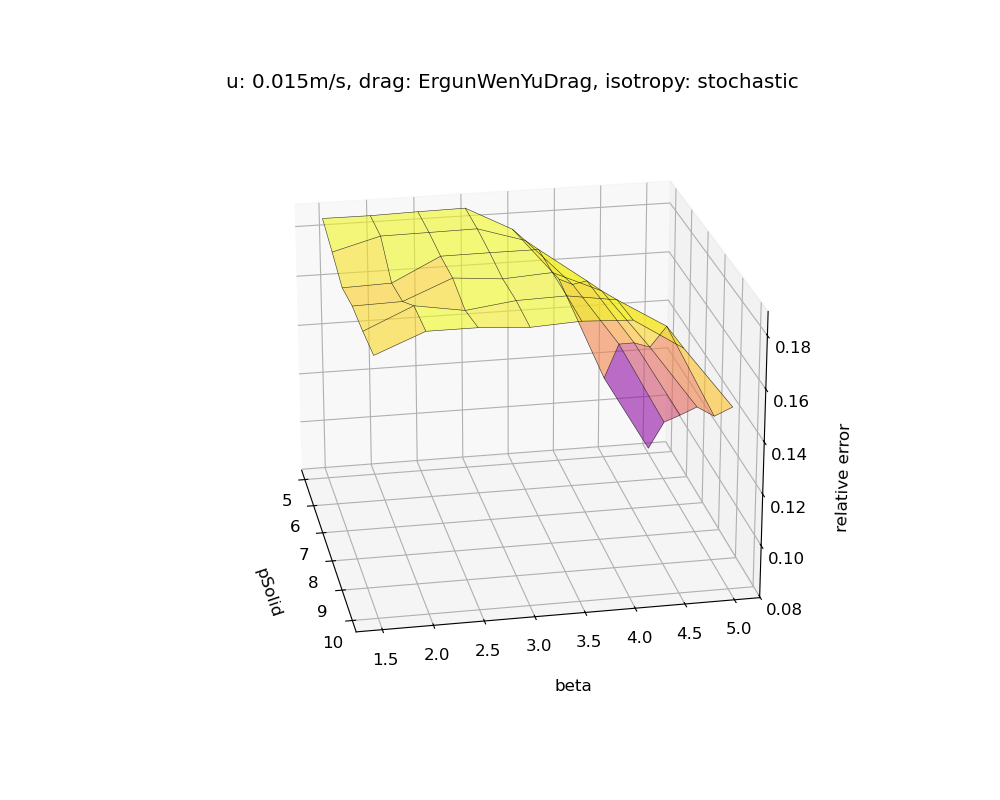
\includegraphics[width = \linewidth, trim = {3.5cm 0 3.5cm 0}, clip]{sections/result/Case3Kin/kin_Z_height0.015_ErgunWenYuDrag_stochastic.png}
        \caption{Relative error of bed height with drag model \lstinline|ErgunWenYuDrag|, isotropy model \lstinline|stochastic| and inlet velocity $0.015m/s$.}
    \end{subfigure}
\end{figure}

\begin{figure}[h!]
    \centering
    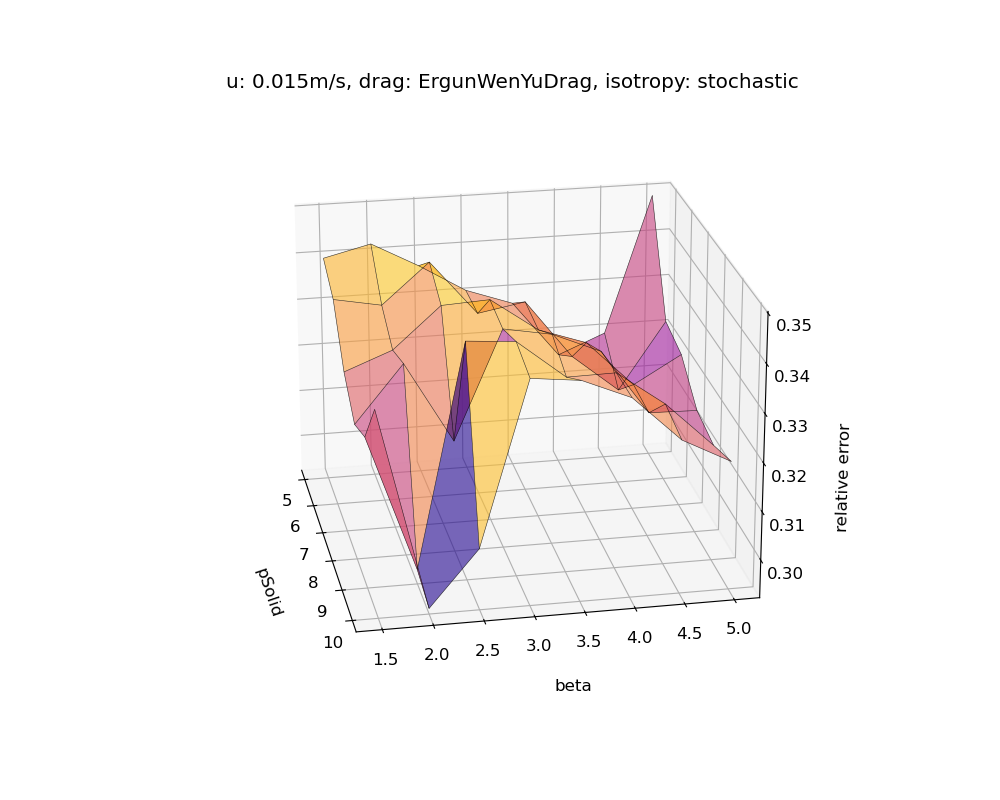
\includegraphics[width=0.5\linewidth, trim = {3.5cm 0 3.5cm 0}, clip]{sections/result/Case3Kin/kin_Z_both0.015_ErgunWenYuDrag_stochastic.png}
    \caption{Combined relative error with drag model \lstinline|ErgunWenYuDrag|, isotropy model \lstinline|stochastic| and inlet velocity $0.015m/s$, according to equation \eqref{eq:relError}.}
    \label{fig:placeholder}
\end{figure}
\FloatBarrier


For the \lstinline
|ErgunWenYuDrag| model with and without the isotropy model we can observe spikes for the combination of high pressure constants and low exponents and for the opposite case of high exponents and low pressure constants.
These are more prevalent when the isotropy model is turned on.
The isotropy model has no significant effect on the relative error of the bed height.

\paragraph{Drag model \lstinline|PlessisMaliyahDrag| and isotropy model \lstinline|none|}

We convert the drag model to the \lstinline|PlessisMaliyahDrag| model. 
The previously observed spike in pressure drop error for large exponents and small pressure constants can still be found at $\beta = 5$ and $P_s = 5$ with a relative error of $0.33$.
As seen before with the \lstinline|ErgunWenYuDrag| model with no isotropy model the minimal error of $0.26$ is adjacent to the maximal error at $\beta = 4$ and $P_s = 5$. The relative error slightly increases for smaller exponents and larger pressure constants.

The relative error of the bed height shows a similar trend as the previous cases with a plateau forming for large pressure constants and small exponents. Although the trend is similar the relative error is nearly double the value of the \lstinline|ErgunWenYuDrag| model. The plateau contains the maximum relative error of $0.30$ at $\beta = 3$ and $P_s = 8$. The relative error drops off for larger exponents and smaller pressure constants. The minimal relative error is located at $P_s = 5$ and $\beta = 5$ with a minimal error of $0.13$.

The overall relative error shows a similar behavior to the bed height error with the spike of the pressure drop error included for the largest exponents and smallest pressure constants.
The maximum error is located at the top of the plateau where the bed height error is large.
The largest error of $0.41$ is located at $\beta = 2$ and $P_s = 7$.
THe minimum error of $0.32$ is located just before the spike at $\beta = 5$ and $P_s = 9$.

\ifcode
\begin{lstlisting}
    5
0
4.0
5.0
0.26053141002337027
7
0
5.0
5.0
0.3313403179915781
0.015_PlessisMasliyahDrag_none.png
7
0
5.0
5.0
0.13205909277439307
3
3
3.0
8.0
0.2978234792764922
0.015_PlessisMasliyahDrag_none.png
7
4
5.0
9.0
0.32783221269938484
1
2
2.0
7.0
0.41354204451578763
0.015_PlessisMasliyahDrag_none.png
\end{lstlisting}
\fi

\FloatBarrier
\begin{figure}[h!]
    \centering
    \begin{subfigure}[b]{0.49 \linewidth}
        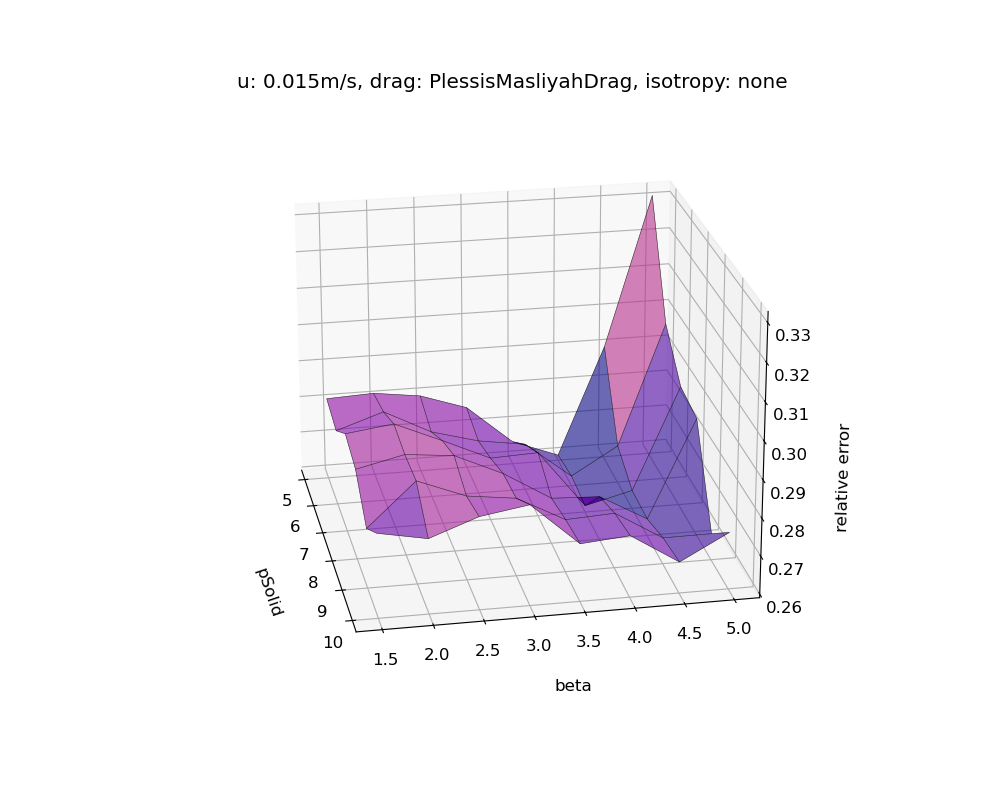
\includegraphics[width = \linewidth, trim = {3.5cm 0 3.5cm 0}, clip]{sections/result/Case3Kin/kin_Z_pres0.015_PlessisMasliyahDrag_none.png}
        \caption{Relative error of pressure with drag model \lstinline|PlessisMasliyahDrag|, isotropy model \lstinline|none| and inlet velocity $0.015m/s$.}
    \end{subfigure}
    \hfill
    \begin{subfigure}[b]{0.49 \linewidth}
        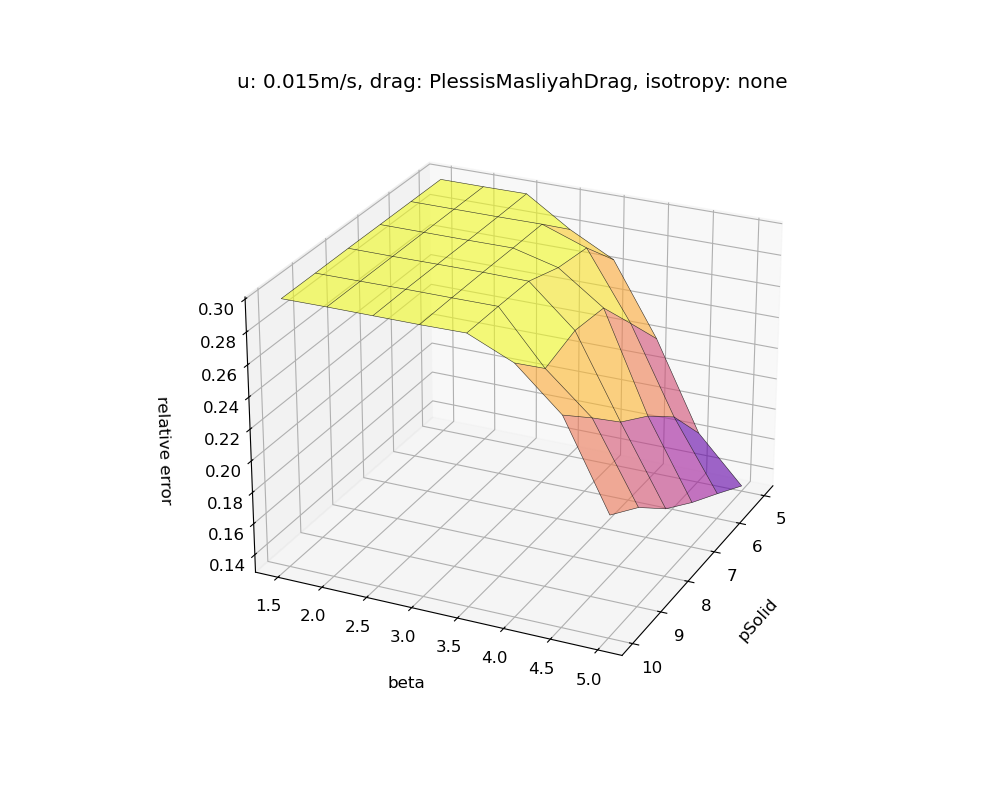
\includegraphics[width = \linewidth, trim = {3.5cm 0 3.5cm 0}, clip]{sections/result/Case3Kin/kin_Z_height0.015_PlessisMasliyahDrag_none.png}
        \caption{Relative error of bed height with drag model \lstinline|PlessisMasliyahDrag|, isotropy model \lstinline|none| and inlet velocity $0.015m/s$.}
    \end{subfigure}
\end{figure}

\begin{figure}[h!]
    \centering
    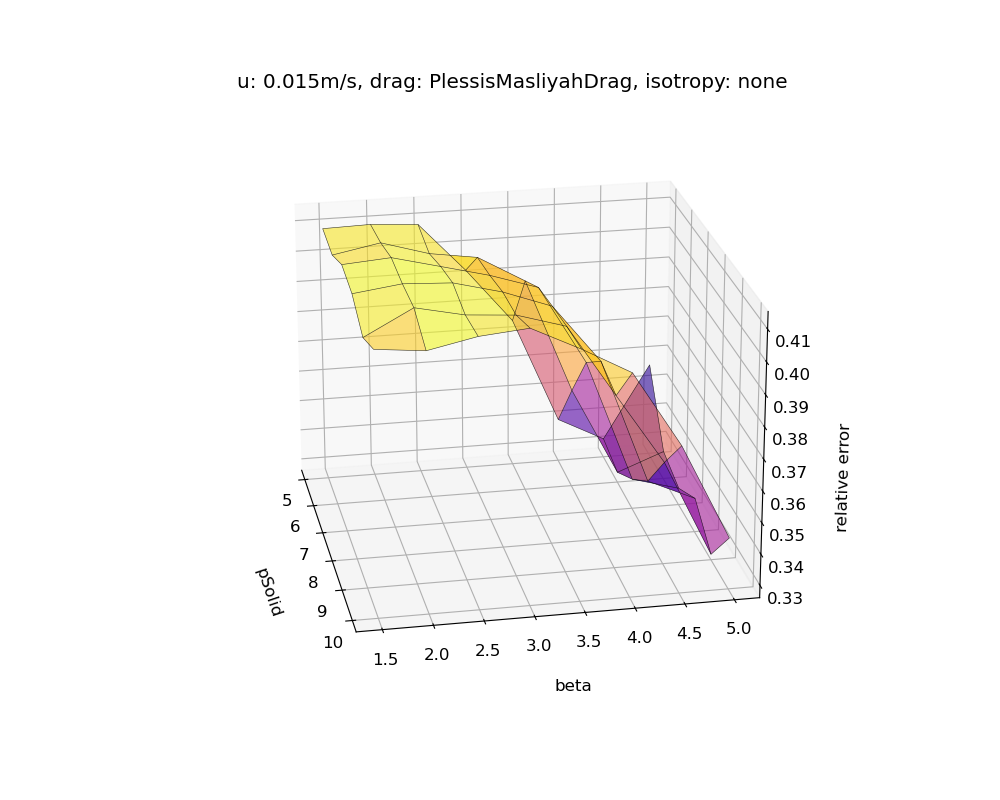
\includegraphics[width=0.5\linewidth, trim = {3.5cm 0 3.5cm 0}, clip]{sections/result/Case3Kin/kin_Z_both0.015_PlessisMasliyahDrag_none.png}
    \caption{Combined relative error with drag model \lstinline|PlessisMasliyahDrag|, isotropy model \lstinline|none| and inlet velocity $0.015m/s$, according to equation \eqref{eq:relError}.}
    \label{fig:placeholder}
\end{figure}
\FloatBarrier



\paragraph{Drag model \lstinline|PlessisMaliyahDrag| and isotropy model \lstinline|stochastic|}

We turn the isotropy model back on.
The pressure drop error height decreases slightly but fluctuates more.
The relative error tends to increase for larger exponents. The peak is located at $P_s = 5$ and $\beta = 5$ with a relative error of $0.30$.
At the smallest exponent of $\beta = 1.5$ the minimum is located at $P_s = 6$ with a value of $0.24$.

The behavior of the bed height remains mostly unaltered.
The maximal error of $0.30$ is located on the plateau that forms for lower exponents at $\beta = 2.5$ and $P_s = 5$.
For larger exponents the bed height error again declines. The minimum is located at $P_s =5$ and $\beta = 5$ witha  value of $0.12$.

The overall relative error is a combination of both behaviors. We once again see the decline of the bed heigth for larger exponents and smaller pressure constants. The minimum is located at $\beta = 5$ and $P_s = 6$.
The maximum error is on the plateau at $\beta = 2.5$ and $P_s = 9$ with an error of $0.41$.

\ifcode
\begin{lstlisting}
    0
1
1.5
6.0
0.24202333689226926
7
0
5.0
5.0
0.29715021285073046
0.015_PlessisMasliyahDrag_stochastic.png
7
0
5.0
5.0
0.1244041794248556
2
0
2.5
5.0
0.3029136020707723
0.015_PlessisMasliyahDrag_stochastic.png
7
1
5.0
6.0
0.3210105860281726
2
4
2.5
9.0
0.4146076811383962
0.015_PlessisMasliyahDrag_stochastic.png
\end{lstlisting}
\fi
\FloatBarrier
\begin{figure}[h!]
    \centering
    \begin{subfigure}[b]{0.49 \linewidth}
        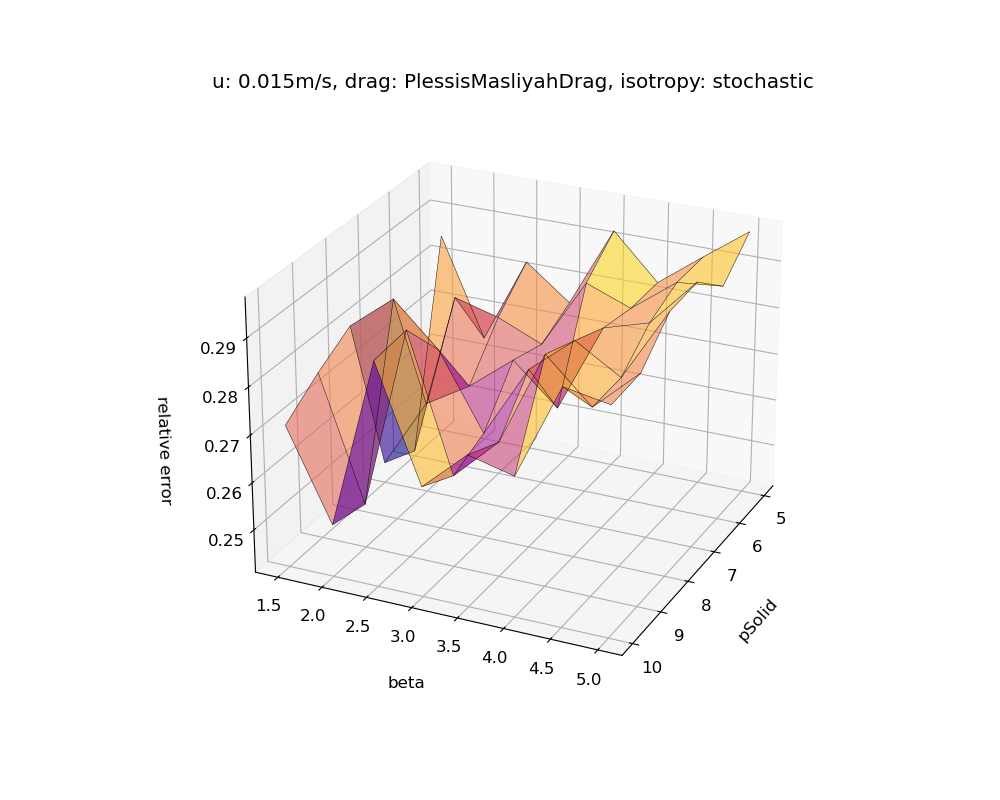
\includegraphics[width = \linewidth, trim = {3.5cm 0 3.5cm 0}, clip]{sections/result/Case3Kin/kin_Z_pres0.015_PlessisMasliyahDrag_stochastic.png}
        \caption{Relative error of pressure with drag model \lstinline|PlessisMasliyahDrag|, isotropy model \lstinline|none| and inlet velocity $0.015m/s$.}
    \end{subfigure}
    \begin{subfigure}[b]{0.49 \linewidth}
        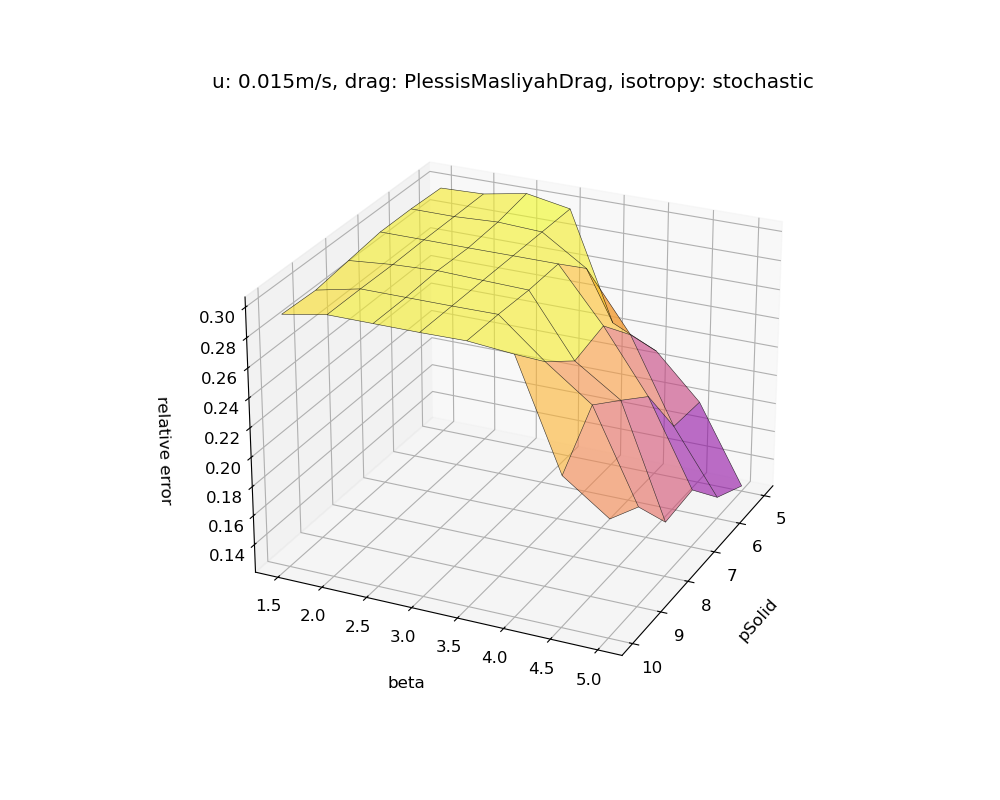
\includegraphics[width = \linewidth, trim = {3.5cm 0 3.5cm 0}, clip]{sections/result/Case3Kin/kin_Z_height0.015_PlessisMasliyahDrag_stochastic.png}
        \caption{Relative error of bed height with drag model \lstinline|PlessisMasliyahDrag|, isotropy model \lstinline|stochastic| and inlet velocity $0.015m/s$.}
    \end{subfigure}
\end{figure}

\begin{figure}[h!]
    \centering
    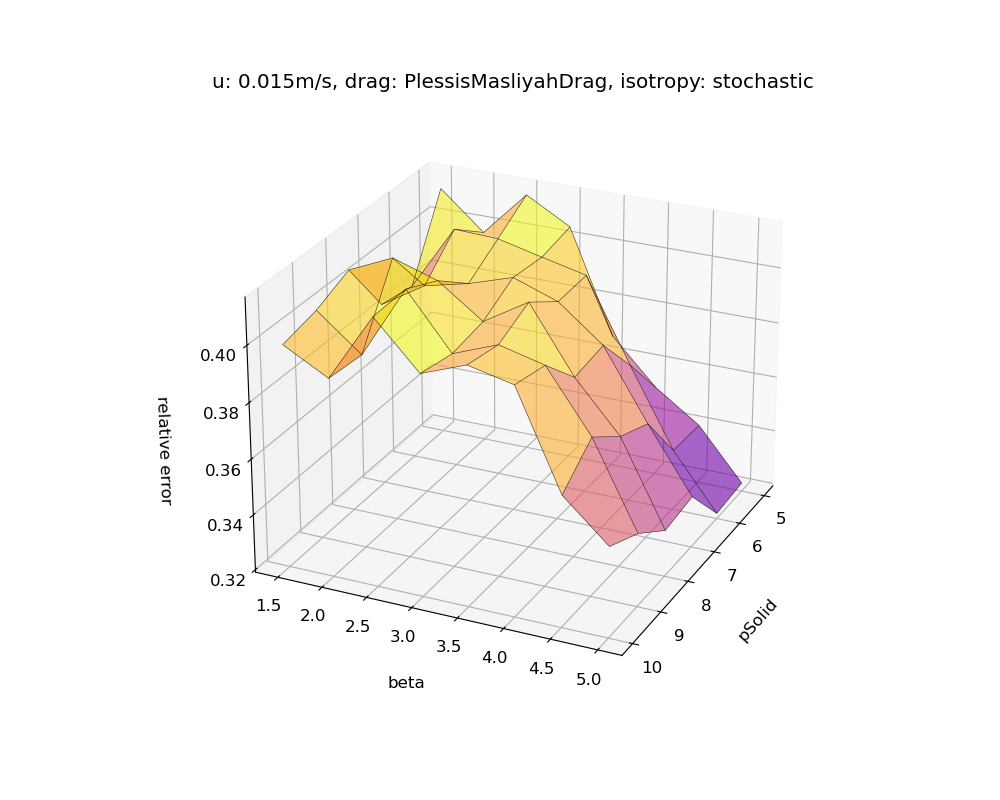
\includegraphics[width=0.5\linewidth, trim = {3.5cm 0 3.5cm 0}, clip]{sections/result/Case3Kin/kin_Z_both0.015_PlessisMasliyahDrag_stochastic.png}
    \caption{Combined relative error with drag model \lstinline|PlessisMasliyahDrag|, isotropy model \lstinline|stochastic| and inlet velocity $0.015m/s$, according to equation \eqref{eq:relError}.}
    \label{fig:placeholder}
\end{figure}
\FloatBarrier
Overall the \lstinline|PlessisMaliyahDrag| model again showed a higher relative error. 
The bed height is minimized for larger exponents and smaller pressure constants.


\subsection{Discussion and Results}
\label{sec:discAndRes}

Overall we summarize the parameters that lead to the minimal relative error in each case in the following table \ref{tab:minPar}.
\setlength{\tabcolsep}{10pt} % Default value: 6pt
\renewcommand{\arraystretch}{1.25} % Default value: 1
\begin{table}[h!]
    \centering
    \begin{tabular}{c|c c|c c}
         &  \lstinline|PlessisMasliyah| &\lstinline|PlessisMasliyah| & \lstinline|ErgunWenYu| & \lstinline|ErgunWenYu|\\
         & \lstinline|stochastic| & \lstinline|none| & \lstinline|stochastic| & \lstinline|none| \\
         \hline
         Case 1 & \shortstack{$\beta = 5 $ \\ $\pvfcp = 0.7$ \\ $err_{min} = 0.30$}& \shortstack{$\beta = 5 $ \\ $\pvfcp = 0.68$ \\ $err_{min} = 0.29$} & \shortstack{$\beta = 2 $ \\ $\pvfcp = 0.65$\\ $err_{min} = 0.25$} & \shortstack{$\beta = 4.5 $ \\ $\pvfcp = 0.7$\\ $err_{min} = 0.26$} \\
         \hline
         Case 2 & \shortstack{$P_s = 10$ \\$\pvfcp = 0.63$\\ $err_{min} = 0.33$} & \shortstack{$P_s = 7$ \\ $\pvfcp = 0.65$\\ $err_{min} = 0.36$} & \shortstack{$P_s  = 10$ \\ $\pvfcp = 0.65$\\ $err_{min} = 0.25$} & \shortstack{$P_s = 9$ \\ $\pvfcp = 0.55$\\ $err_{min} = 0.29$} \\
         \hline
         Case 3 & \shortstack{$P_s = 10$ \\ $\beta = 2$\\ $err_{min} = 0.29$} & \shortstack{$P_s = 6$ \\ $\beta = 5$\\ $err_{min} = 0.32$} & \shortstack{$P_s = 10$ \\ $\beta =2$\\ $err_{min} = 0.29$} & \shortstack{$P_s = 5$ \\ $\beta = 4.5$\\ $err_{min} = 0.29$}
    \end{tabular}
    \caption{Parameters for minimal relative error for each case.}
    \label{tab:minPar}
\end{table}


As we saw in the 
The \lstinline|ErgunWenYuDrag| model consistently outperforms the \lstinline|PlessisMasliyahDrag| model.
The mean bed height is higher when the \lstinline|PlessisMasliyahDrag| model is used leading to almost twice the relative error and therefor a higher combined relative error.
Both the pressure drop and the bed height exceed the values from the given data. 
\Todo{Grafik mit gemittelter Betthöhe und Pressure drop}




The error that is consistently the lowest is that of the \lstinline|ErgunWenYuDrag| model with the isotropy model \lstinline|stochastic|.
In this case the minimizing parameters are the same for all three cases, namely $\beta = 2$, $\pvfcp = 0.65$, $P_s = 10$ which happens to coincide with the parameters of the standard \lstinline|Goldschmidt| case. \todo{Das macht irgendwie die Simulationen die ich noch laufen lassen wollte redundant :(}

The pressure drop relative error often ranged no more than $0.04$ in our parameter study, leaving little opportunity for adapting the parameters to fit the experiment.

Multiple error sources skew the parameter study.
The bed height calculated from the experimental videos is debatable.
The method here of counting pixels for a bed height of $1cm$ and dividing the pixel height in the following images.
For the bed height of $1cm$ we settle on $31$ pixels but estimate an error range of $3$ pixels, almost $10 \%$.
On top of in certain cases distinguishing between dust from the particles and the particles proves to be nearly impossible and the images sometimes wobble.
The algorithm therefor sometimes provides wrong bed heights.
Therefor the accuracy of the experimental bed height used here needs to be revisited.

Comparing pressure from the simulation to the experiments is only partially useful. This is due to the locations where data was collected in the experiments compared to the simulation.
In the experiments pressure is measured beneath the mesh.
In the simulation we do not simulate beneath the mesh. Simulations that included the region beneath the mesh showed unphysical interactions between the baffle used to imitate the mesh and the particles. 
In this simulation we therefor reverted to measuring the pressure near the top of the simulation and near the bottom. We expect the pressure to be higher at the bottom of the bed than what is measured beneath the bed.
Although the simulation and experiments do not yield a coinciding result it is unclear whether the \MP method is not capable of predicting the pressure drop accurately.















\section{Limitation of the \MP method}
\begin{footcitedquote}[{will, manager of \OF, \url{https://bugs.openfoam.org/view.php?id=3165}}]
    You have not described a bug. MPPIC modeling has its limitations, and if your simulation is failing because of them then your usage is in error.  
\end{footcitedquote}
%\url{https://bugs.openfoam.org/view.php?id=3165}

Although the \MP method shows promising results for modeling fluidized beds, there are cases in which due to the modeling assumptions the \MP method shows non-physical results.
One example would be simulating a fixed bed.
Inserting particles into a reactor with no fluid inlet velocity we would expect the particles to fall down and lay flat with no velocity.
If we simulate this case with \lstinline|MPPICFoam| with gas inlet velocity of $10^{-6} m/s$ and calculate the average absolute velocity of the particles after five seconds they still have a mean velocity of $0.2m/s$.
Because of the close packing in the cells the particle normal stress is high and the particles are constantly accelerated. The particles move within the bed.
We track one of the particles over the first two seconds. %Particle ID 144135
The particle moves from the right hand side of the simulation to the left hand side. After the particles have fallen down and should be at rest the partilce travels upward inside the bed.
\begin{figure}[h!]
    \centering
    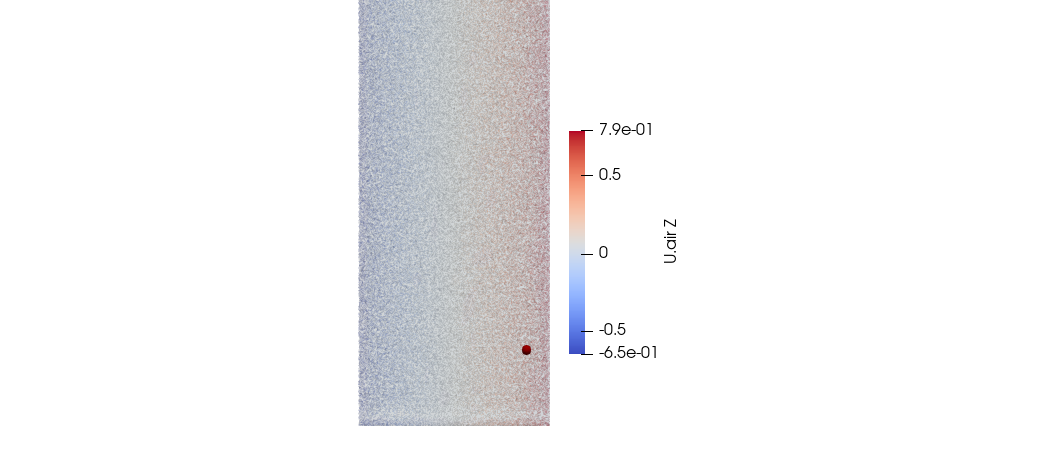
\includegraphics[width=0.3\linewidth, trim = {12cm 0 12cm 0}, clip]{sections/result/particle_bed_moves_too_much/part_move_144135.0000.png}
    \hfill
    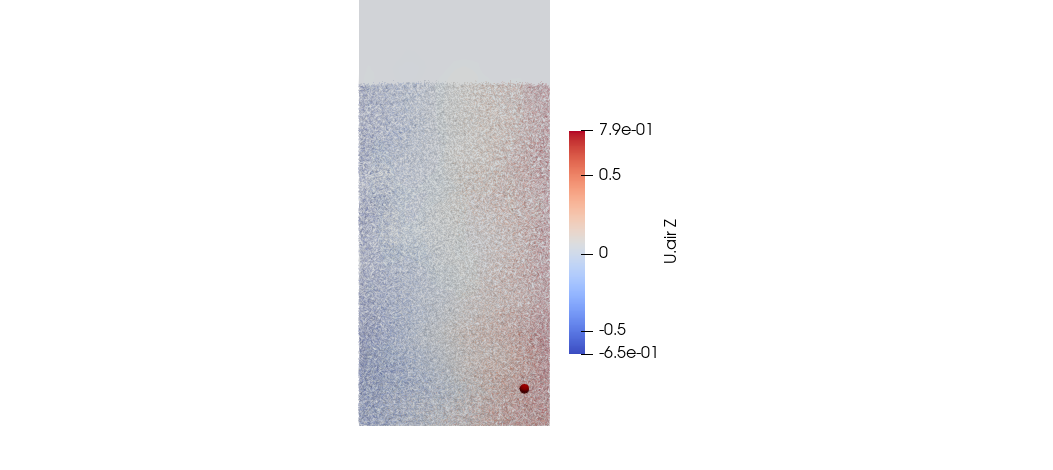
\includegraphics[width=0.3\linewidth, trim = {12cm 0 12cm 0}, clip]{sections/result/particle_bed_moves_too_much/part_move_144135.0015.png}
    \hfill
    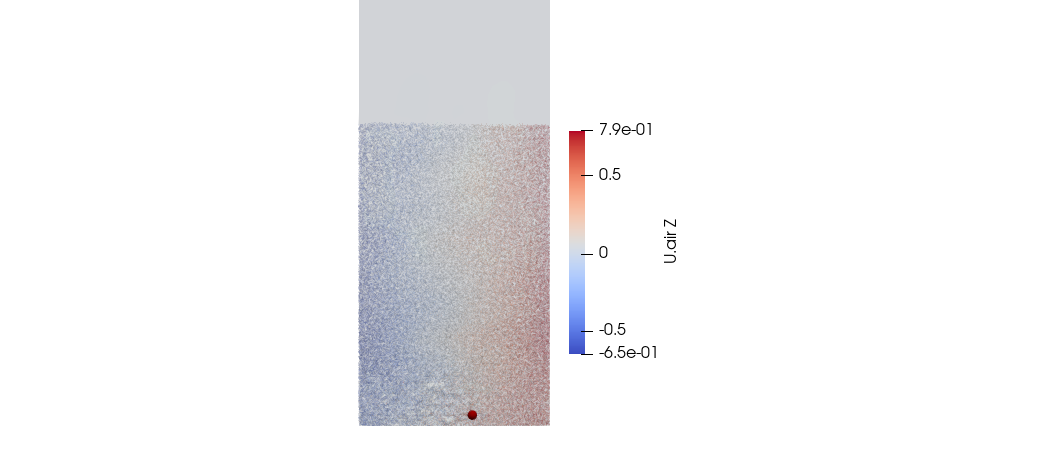
\includegraphics[width=0.3\linewidth, trim = {12cm 0 12cm 0}, clip]{sections/result/particle_bed_moves_too_much/part_move_144135.0020.png}
    \hfill
    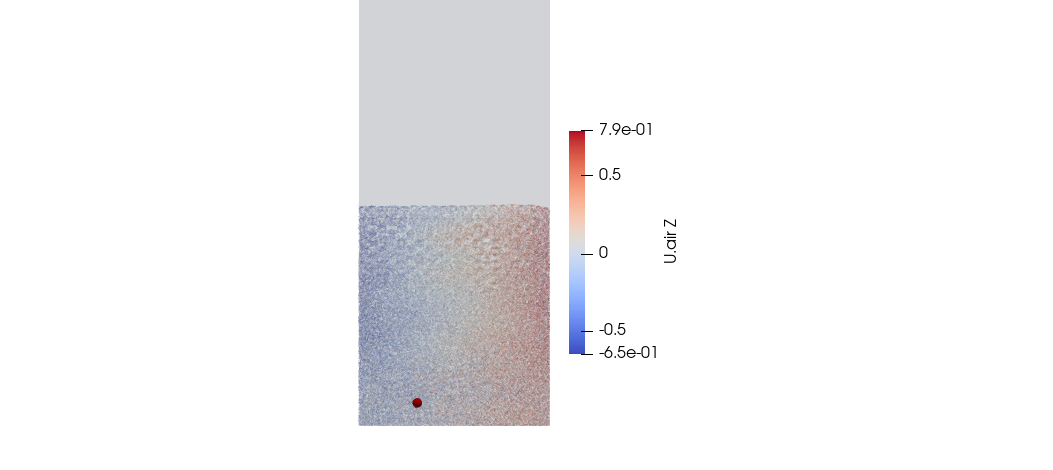
\includegraphics[width=0.3\linewidth, trim = {12cm 0 12cm 0}, clip]{sections/result/particle_bed_moves_too_much/part_move_144135.0040.png}
    \hfill
    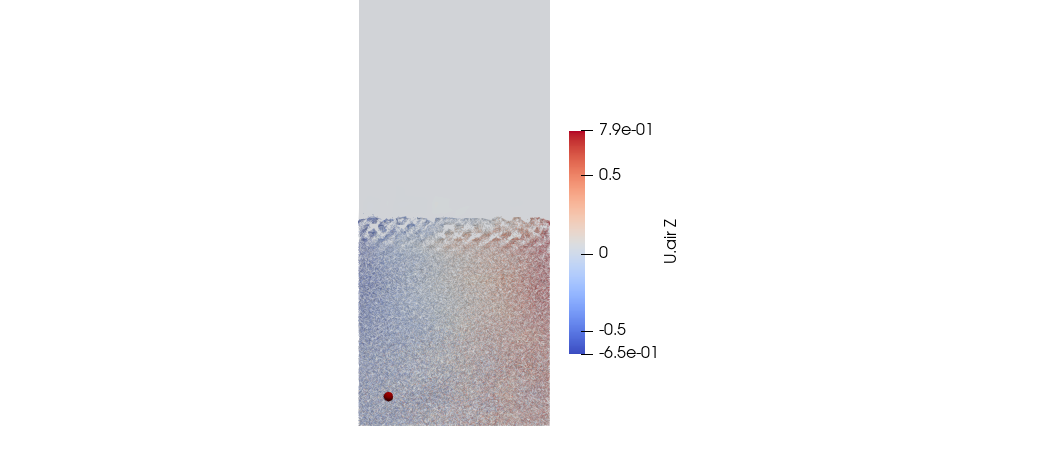
\includegraphics[width=0.3\linewidth, trim = {12cm 0 12cm 0}, clip]{sections/result/particle_bed_moves_too_much/part_move_144135.0060.png}
    \hfill
    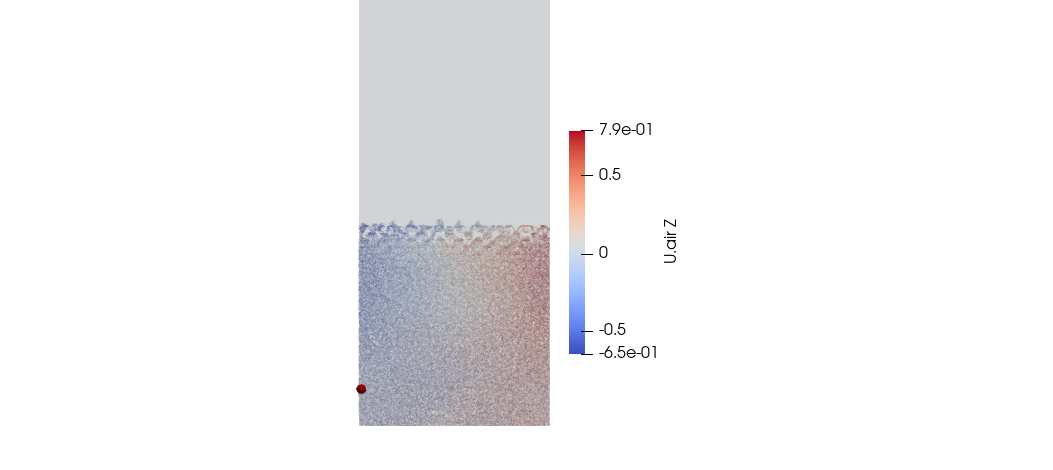
\includegraphics[width=0.3\linewidth, trim = {12cm 0 12cm 0}, clip]{sections/result/particle_bed_moves_too_much/part_move_144135.0080.png}
    \caption{Particle with ID $144135$ after $0s$, $0.5s$, $0.625s$, $1s$, $1.5s$, $2s$. The particle should be at rest after the first second but still moves.}
    \label{fig:part_moves_packed}
\end{figure}



%\Todo{Color one particle in the reactor}

